\documentclass[aspectratio=169]{beamer}
\usepackage{hyperref}
\usepackage[T1]{fontenc}
\usepackage{newtxtext,newtxmath}
\makeatletter
\def\input@path{{}{3. Presentacion/}}
\makeatother
\usepackage{tribhuvan}
\usepackage[absolute,overlay]{textpos}
\usepackage[table]{xcolor}

% Recuerda incluir \usepackage{xcolor, booktabs, ulem} en tu preámbulo si no los tienes
\definecolor{llamativoMagenta}{rgb}{0.0, 0.28, 0.67} 
\newcommand{\contrib}[1]{\textcolor{llamativoMagenta}{\textbf{\underline{#1}}}}


% other packages
\usepackage{latexsym,amsmath,xcolor,multicol,booktabs,calligra}
\usepackage{graphicx,pstricks,listings,stackengine}
\graphicspath{{figures_optimized/}{../figures_optimized/}{../../figures_optimized/}{figures/}{../figures/}{../../figures/}}
\makeatletter
\newcounter{prismfigure}
\renewcommand{\theprismfigure}{\arabic{prismfigure}}
\providecommand{\theHprismfigure}{\arabic{prismfigure}}
\let\prism@original@includegraphics\includegraphics
\renewcommand{\includegraphics}[2][]{%
    \prism@original@includegraphics[#1]{#2}%
    \refstepcounter{prismfigure}%
    \label{fig:auto-\theprismfigure}%
}
\makeatother

\author[Carlos Benítez]{Carlos Benítez}
\title[Ingeniería Mecatrónica]{Avances del prototipo de procesamiento local para detecci\'on, clasificaci\'on y an\'alisis predictivo de manchas solares}
\subtitle{Informe de avance para tutor\'ia}
\institute[FIUNA]{Universidad Nacional de Asunci\'on \\ Facultad de Ingenier\'ia \\ Ingenier\'ia Mecatr\'onica}
\date{13 de abril de 2026}


% defs
\def\cmd#1{\texttt{\color{red}\footnotesize $\backslash$#1}}
\def\env#1{\texttt{\color{blue}\footnotesize #1}}
\definecolor{deepblue}{rgb}{0,0,0.5}
\definecolor{deepred}{rgb}{0.6,0,0}
\definecolor{deepgreen}{rgb}{0,0.5,0}
\definecolor{halfgray}{gray}{0.55}

\lstset{
    basicstyle=\ttfamily\small,
    keywordstyle=\bfseries\color{deepblue},
    emphstyle=\ttfamily\color{deepred},    % Custom highlighting style
    stringstyle=\color{deepgreen},
    numbers=left,
    numberstyle=\small\color{halfgray},
    rulesepcolor=\color{red!20!green!20!blue!20},
    frame=shadowbox,
}

\renewcommand{\familydefault}{\rmdefault}
\setbeamerfont{title}{size=\Large}
\setbeamerfont{subtitle}{size=\normalsize}
\setbeamerfont{author}{size=\normalsize}
\setbeamerfont{institute}{size=\small}
\setbeamerfont{date}{size=\small}

\newcommand{\imageplaceholder}[2][0.95\linewidth]{%
    \fbox{%
        \begin{minipage}[c][0.20\textheight][c]{#1}
            \centering
            \textbf{[Imagen pendiente]}\\[4pt]
            \footnotesize #2
        \end{minipage}%
    }%
}

\AtBeginSubsection[]{}


\begin{document}

\begin{frame}[plain]
    \centering
    \vfill % Distribuye el espacio vertical superior

    % Línea superior de enmarque elegante
    {\color{granate}\rule{0.85\linewidth}{1.2pt}\par}
    \vspace{0.35cm}

    % Título optimizado: tamaño reducido a \normalsize para equilibrar el peso visual
    \begin{minipage}{0.85\linewidth}
        \centering
        {\normalsize\bfseries\color{rojo-oscuro} Desarrollo de un Prototipo de Procesamiento Local\\ para la Detección, Clasificación y Análisis Predictivo de Manchas Solares mediante Visión Computacional e Inteligencia 
Artificial\par}
    \end{minipage}\par

    \vspace{0.35cm}
    
    % Logo institucional centrado
    
\includegraphics[height=2.0cm,keepaspectratio]{logos/fiuna_logo.png}\par 
    
    \vspace{0.35cm}
    
    % Bloque del Autor bien definido
    {\normalsize\bfseries Carlos Benítez\par}
    \vspace{0.1cm}
    {\scriptsize Universidad Nacional de Asunción\par}
    {\scriptsize Facultad de Ingeniería $\cdot$ Ingeniería Mecatrónica\par}

    \vspace{0.4cm}
    
    % Bloque de Tutores optimizado en estructura y legibilidad
    \begin{minipage}{0.90\linewidth} 
        \centering
        {\scriptsize\textbf{\color{rojo-oscuro}Tutores}}\\[4pt] 
        {
        Dr. Juan Carlos Cabral \quad$\cdot$\quad Dr. Diego Stalder \quad$\cdot$\quad Dr. Christian E. Schaerer\\[2pt]
        Dr. José María Gómez \quad$\cdot$\quad MSc. Jesús Núñez
        }
    \end{minipage}
    
    \vfill % Distribuye el espacio hacia la línea inferior
    
    % Línea inferior de cierre
    {\color{granate}\rule{0.85\linewidth}{1.2pt}\par}
    \vspace{0.1cm}
\end{frame}

% \begin{frame}{Contenido}
%     \vspace{0.2cm}
%     \begin{minipage}{0.85\linewidth}
%         \tableofcontents[sectionstyle=show,subsectionstyle=show/shaded/hide,subsubsectionstyle=show/shaded/hide]
%     \end{minipage}
% \end{frame}


\section{Introducción y Objetivos}


\begin{frame}{Introducción: Efectos del clima espacial}
    \centering
    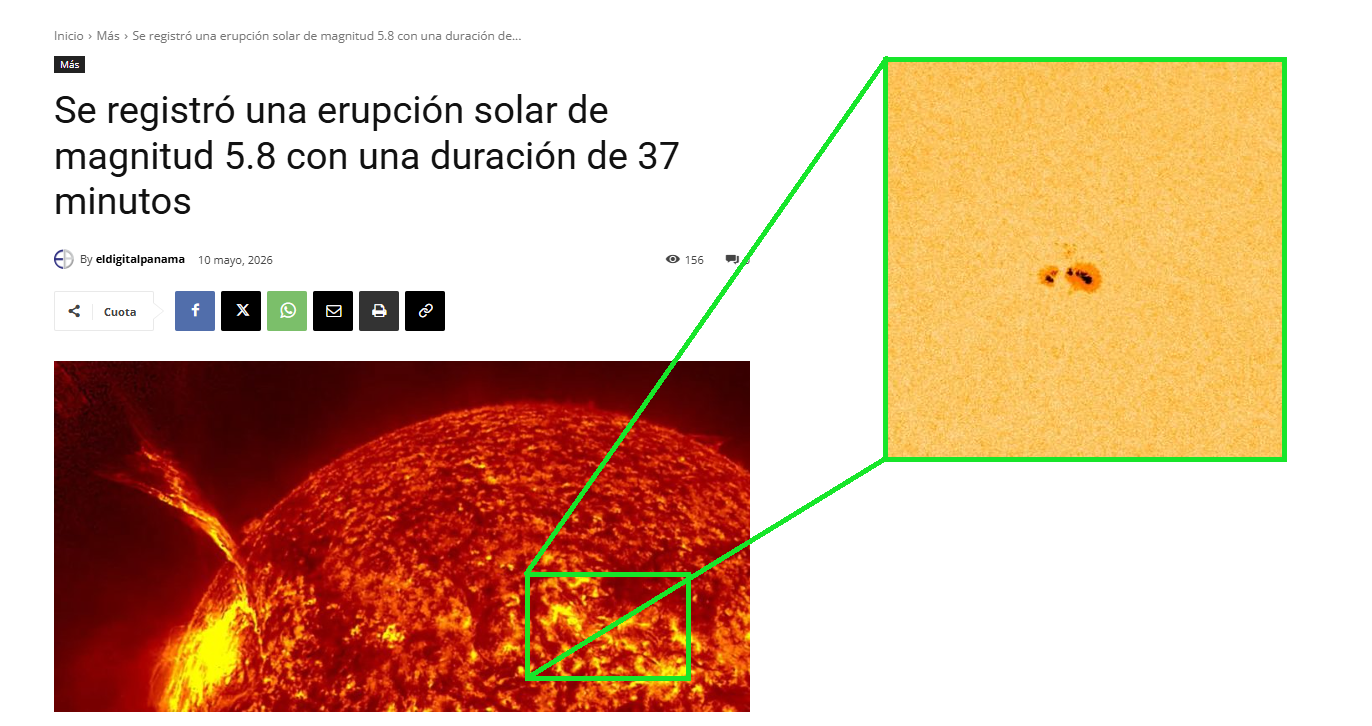
\includegraphics[height=0.75\textheight,width=0.96\linewidth,keepaspectratio]{solar/news.png}\par
    \vspace{0.05cm}
    %{\footnotesize Adaptado de Hathaway [2]}\par
    
    \vfill
    \begin{minipage}{1.0\linewidth}
        \centering\small
       El Instituto de Geofísica Aplicada de Rusia comunicó que el 10 de mayo se registró una erupción solar de magnitud 5.8 de 37 minutos proveniente del grupo de manchas solares 4436.
    \end{minipage}\par
    
    \vspace{0.1cm}
    %{\tiny\color{gray} [2] D. H. Hathaway, “The solar cycle,” Living Reviews in Solar Physics, vol. 12, no. 1, pp. 1--70, 2015.\par}
\end{frame}


\begin{frame}{Introducción: Efectos del clima espacial}
    \centering
    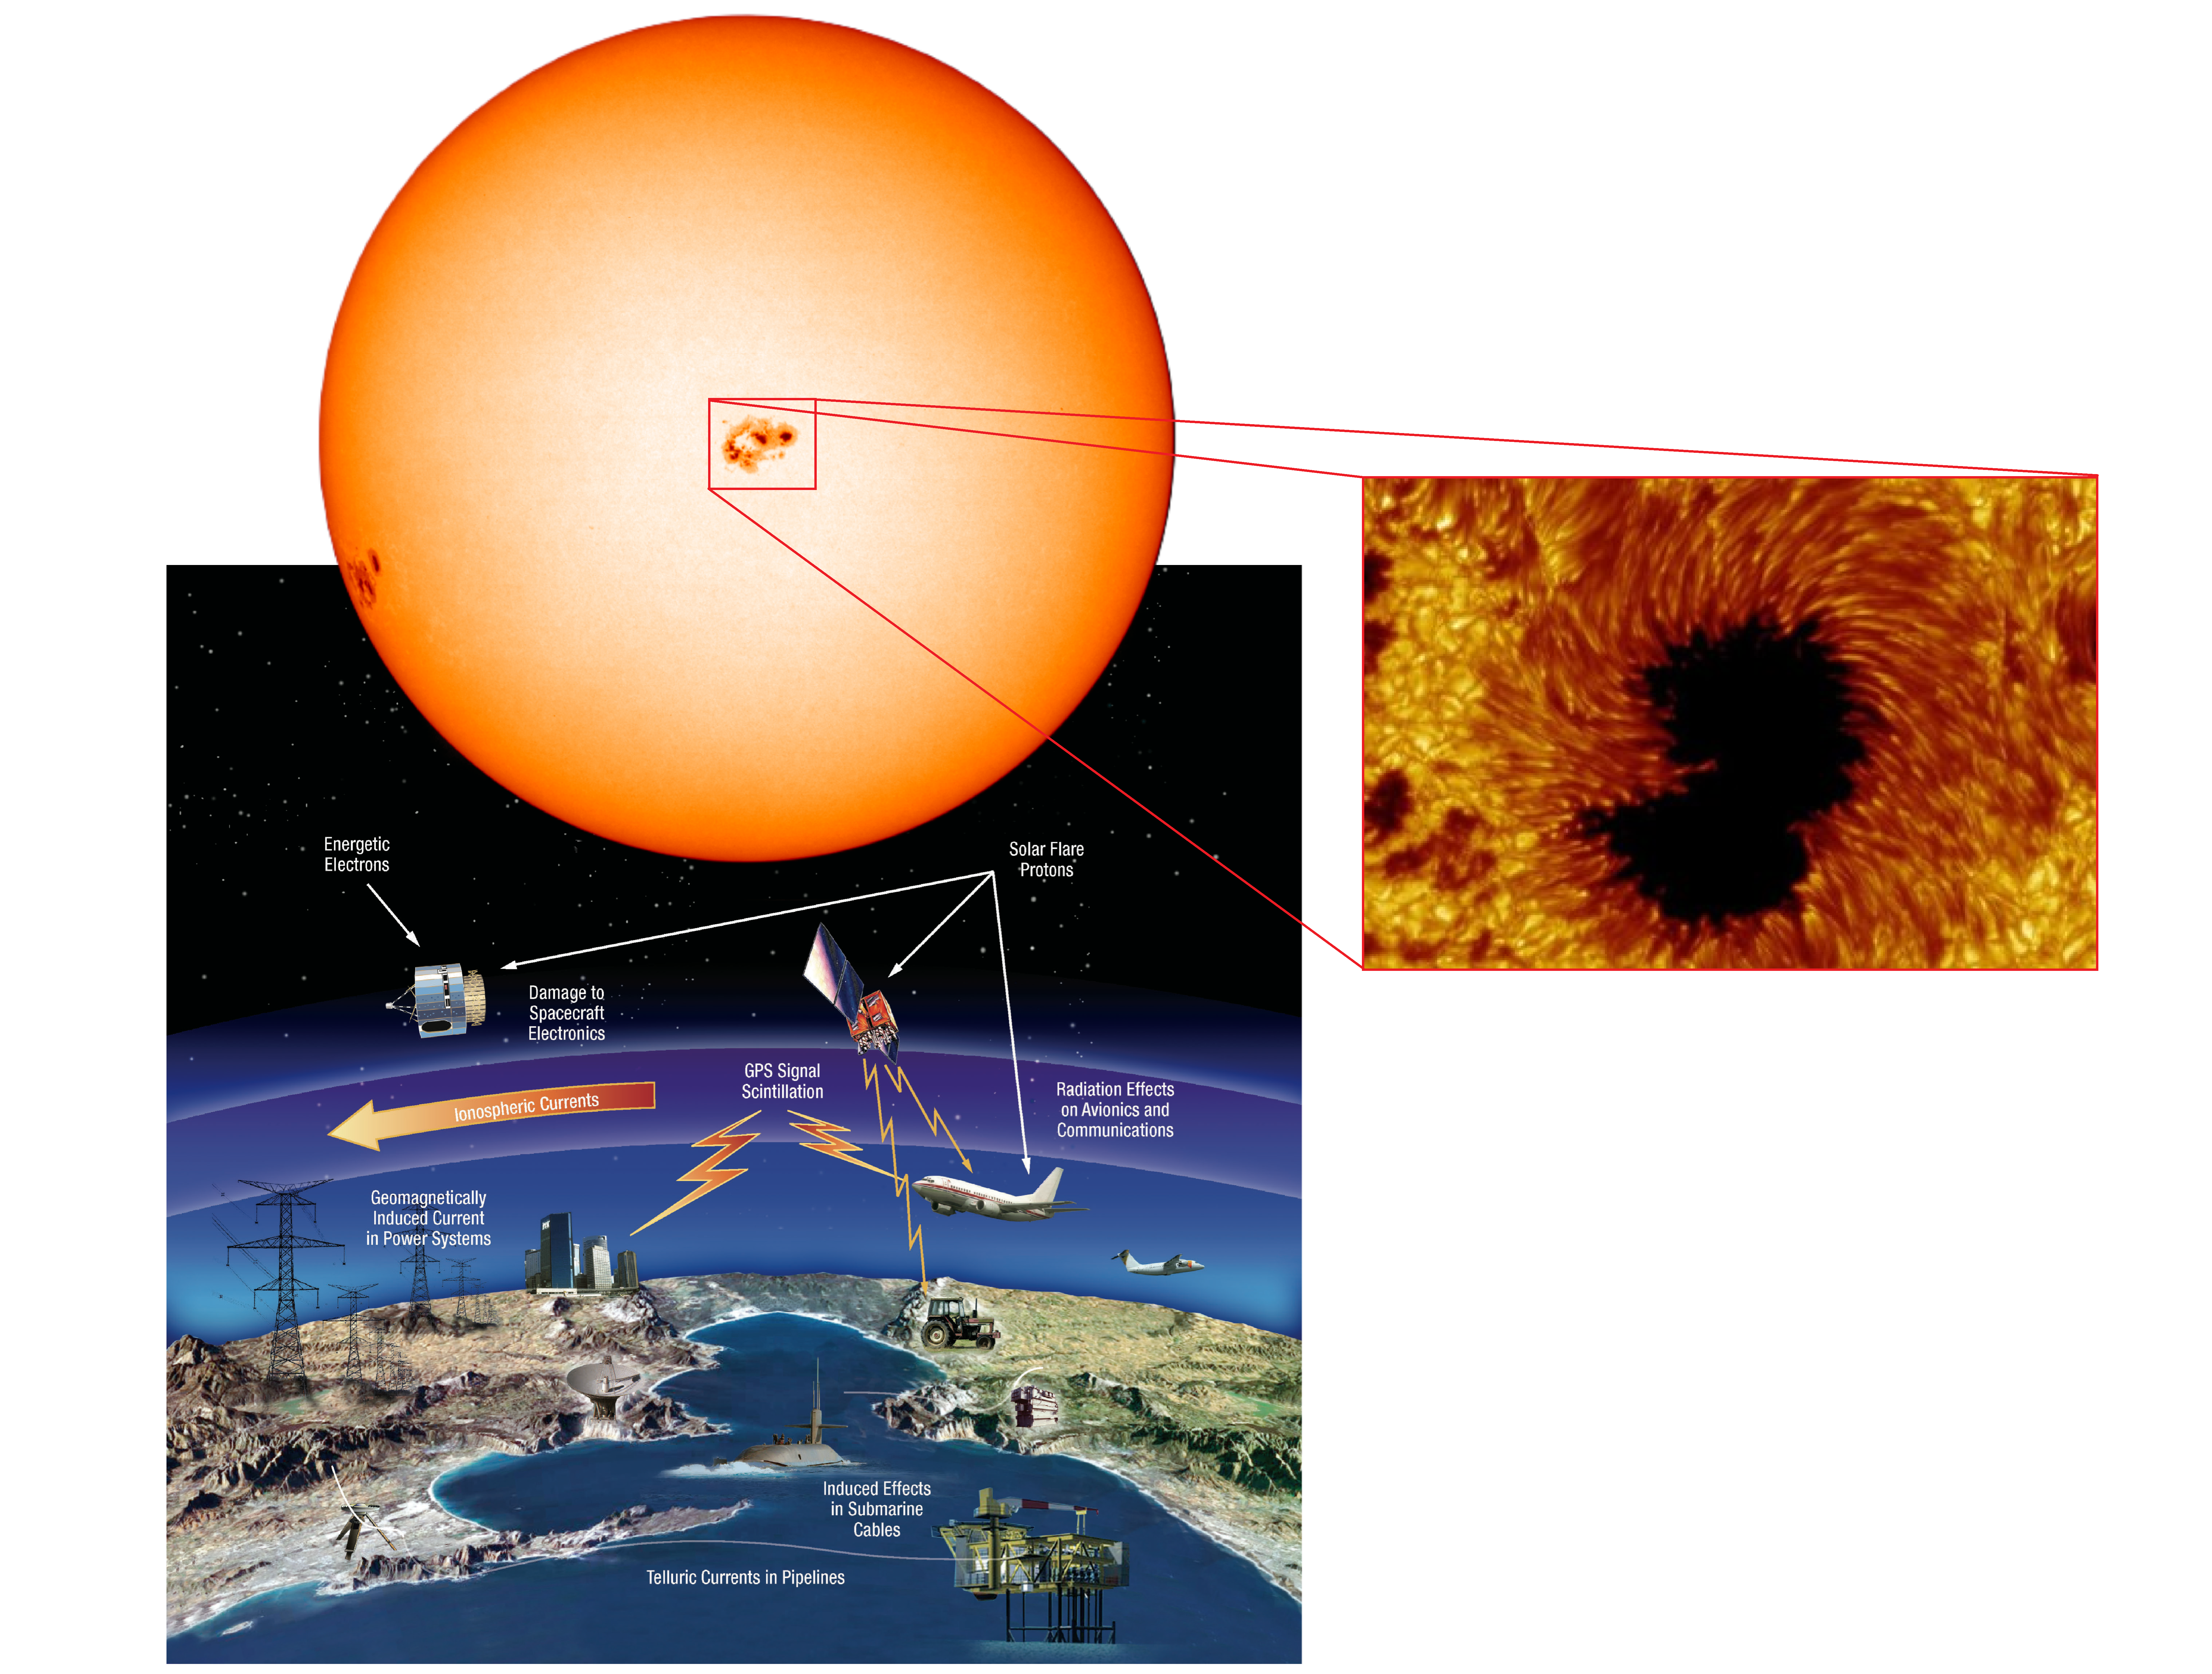
\includegraphics[height=0.55\textheight,width=0.96\linewidth,keepaspectratio]{solar/space-weather-effects.png}\par
    \vspace{0.05cm}
    {\footnotesize NASA Scientific Visualization Studio [1]}\par
    
    \vfill
    \begin{minipage}{0.95\linewidth}
        \centering\small
        Sistemas vulnerables: telecomunicaciones, instrumentación, redes.
    \end{minipage}\par
    
    \vspace{0.1cm}
    {\tiny\color{gray} [1] NASA Scientific Visualization Studio, “Solar Cycle Weather and Atmospheric Forcing Visualizations,” NASA Goddard Space Flight Center, v4.12, 2010.\par}
\end{frame}

% \begin{frame}{Introducción: Clima espacial y sistemas tecnológicos}
%     \centering
%     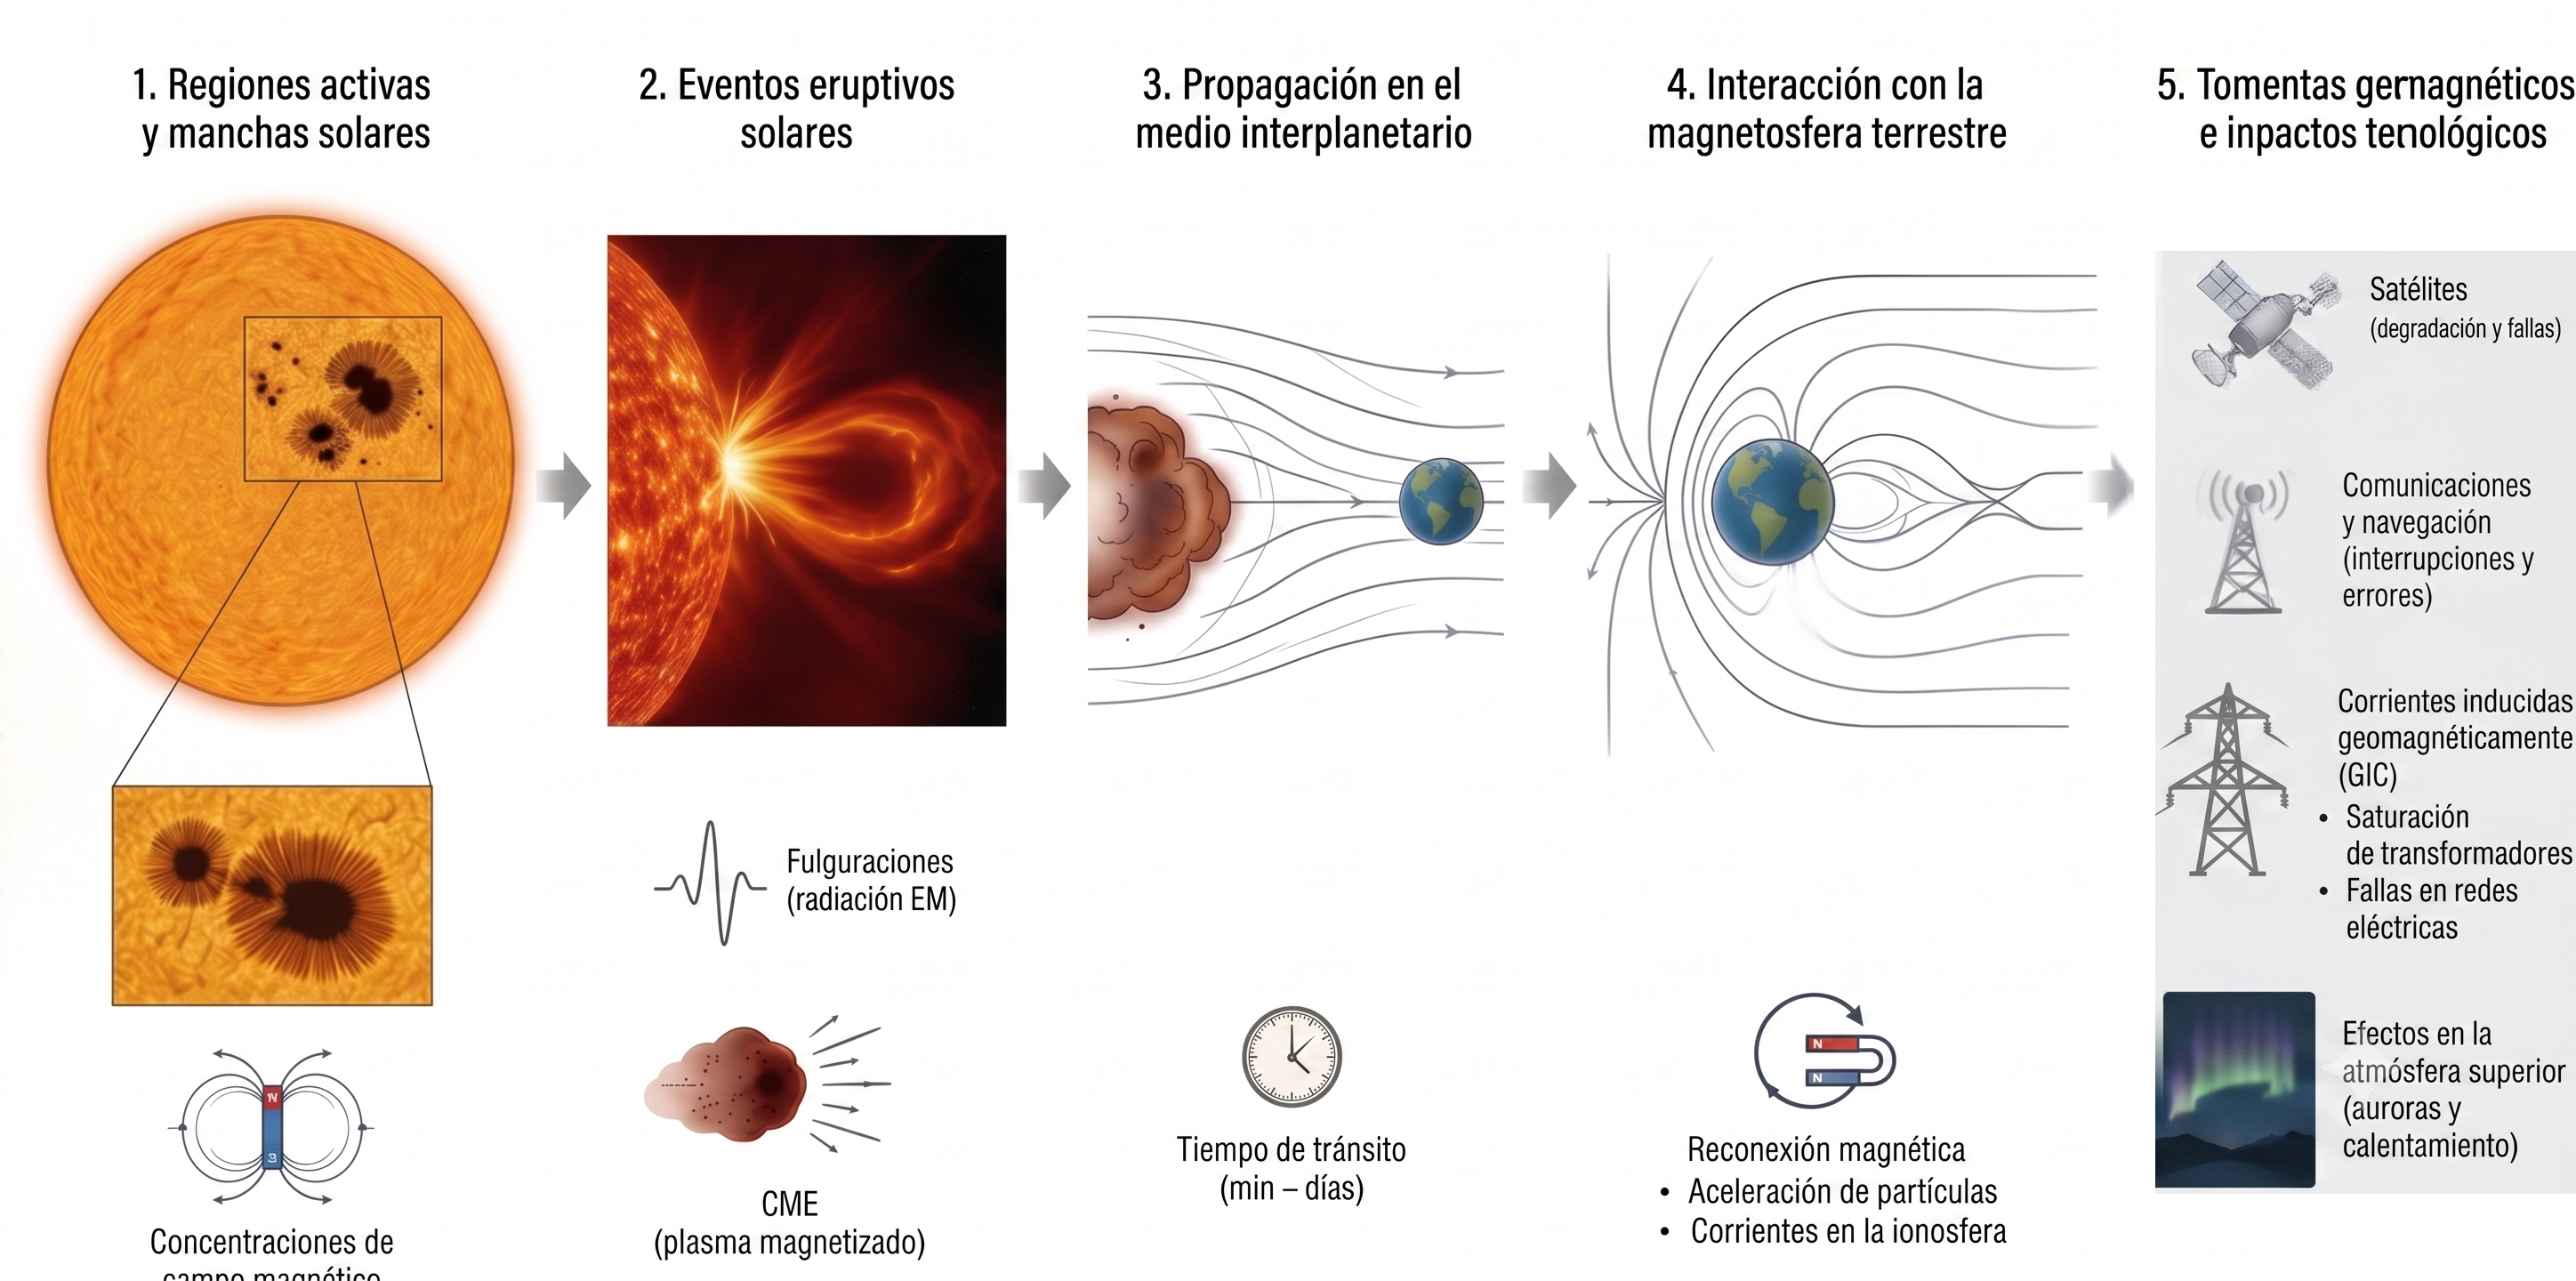
\includegraphics[height=0.65\textheight,width=0.96\linewidth,keepaspectratio]{solar/cycle_solar.png}\par
%     \vspace{0.05cm}
%     %{\footnotesize Adaptado de Hathaway [2]}\par
    
%     \vfill
%     \begin{minipage}{0.95\linewidth}
%         \centering\small
%         Manchas solares: evolución fotosférica. Clima espacial: telecomunicaciones, electrónica y redes. Flujo local: observar, registrar, clasificar, predecir.
%     \end{minipage}\par
    
%     \vspace{0.1cm}
%     %{\tiny\color{gray} [2] D. H. Hathaway, “The solar cycle,” Living Reviews in Solar Physics, vol. 12, no. 1, pp. 1--70, 2015.\par}
% \end{frame}

\begin{frame}{Introducción: Contexto Nacional}
    \centering
    \vfill
    \begin{minipage}{0.75\linewidth}
        \centering
        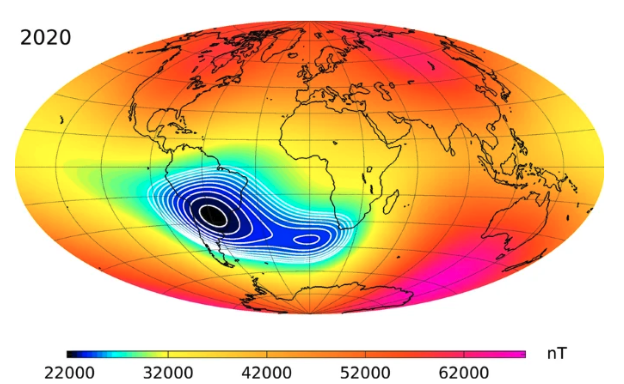
\includegraphics[height=0.66\textheight,keepaspectratio]{solar/south-atlantic-magnetic-anomaly-1.png}\par
        \vspace{0.1cm}
        {\footnotesize Anomalía magnética del Atlántico Sur [2]}
    \end{minipage}\par
    
    \vfill
    {\tiny\color{gray} [2] C. C. Finlay, C. Kloss, N. Olsen, M. D. Hammer, A. Grayver, y A. Kuvshinov, “The CHAOS-7 geomagnetic field model and observed changes in the South Atlantic Anomaly,” Earth, Planets and Space, vol. 72, art. no. 156, 2020.\par}
\end{frame}

\begin{frame}{Introducción: Monitoreo local de manchas solares}
    \centering
    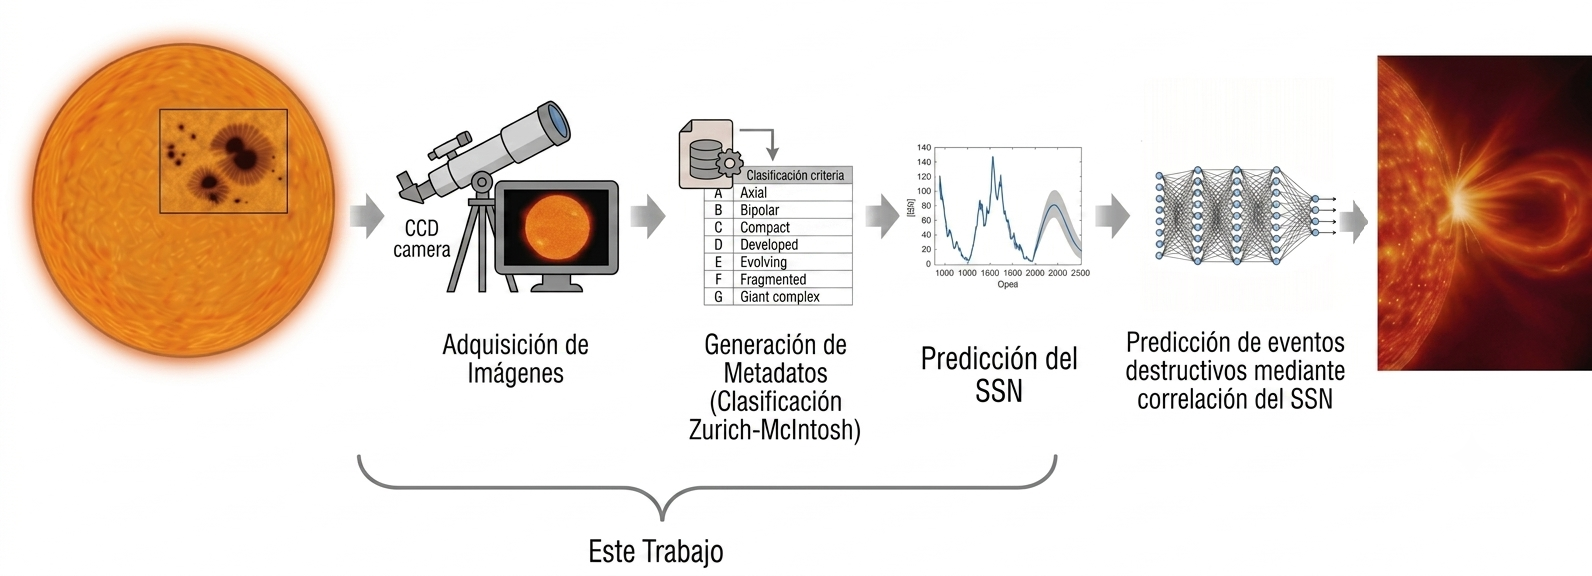
\includegraphics[height=0.65\textheight,width=0.96\linewidth,keepaspectratio]{solar/monitoreo.png}

    \vspace{0.05cm}

    \vfill
    \begin{minipage}{0.95\linewidth}
        \centering\small
        Flujo de trabajo de este proyecto.
    \end{minipage}\par
    
\end{frame}

\begin{frame}{Introducción: Alcance}
    \small
    \vspace{-0.2cm}

    % BLOQUE SUPERIOR: Problemáticas de la Introducción
    \begin{block}{Problemáticas Identificadas}
        \scriptsize
        \begin{itemize}
            \item \textbf{Desafío en Clasificación:} Alta complejidad semántica y estructural en las manchas solares.
            \item \textbf{Vacío Tecnológico:} Ausencia de un ecosistema completo y local de adquisición y registro.
            \item \textbf{Carencia de Datos:} Falta de una base de datos etiquetada bajo estándares internacionales.
        \end{itemize}
    \end{block}

    \vspace{0.1cm}

    % BLOQUE INFERIOR: Respuestas / Contribuciones del trabajo
    \begin{block}{Contribuciones del Trabajo (Soluciones Desarrolladas)}
        \scriptsize
        \begin{enumerate}
            \item \contrib{Dispositivo de Adquisición:} Hardware local y autónomo para captura solar.
            \item \contrib{Base de Datos Etiquetada:} Repositorio estructurado para el entrenamiento de modelos.
            \item \contrib{Modelo DMD--Spörer:} Análisis predictivo de la distribución latitudinal.
            \item \contrib{Clasificador Jerárquico de Deep Learnign:} Clasificador taxonómico Zurich-McIntosh.
            \item \contrib{Framework de Observación:} Sistema integrado híbrido para asistencia en tiempo real.
        \end{enumerate}
    \end{block}
\end{frame}


\begin{frame}{Objetivo General}
    \begin{block}{Objetivo General}
       Desarrollar un prototipo para la detección y clasificación local de manchas solares, integrando técnicas de visión por computadora, inteligencia artificial y análisis predictivo de actividad solar para observatorios locales.
    \end{block}
\end{frame}

\begin{frame}{Objetivos Específicos}
    \centering
    \small
    \begin{enumerate}
            \item Analizar registros historicos de manchas solares a partir de imágenes heliográficas.
            \item Diseñar un flujo de adquisición y preprocesamiento de imágenes para vincular imágenes de manchas solares con reportes internacionales.
            \item Desarrollar un detector basado en arquitecturas de Deep Learning modernas para localizar grupos solares y un clasificador jerárquico de inferencia de caracteres Zurich--McIntosh preservando la dependencias semánticas.
            \item Implementar un módulos predictivo de la evolución temporal del índice de manchas solares y la distribución latitudinal de la actividad a partir de registros históricos.
            \item Integrar el sistema en una arquitectura híbrida con plataforma web y procesamiento inferencial local.
            \item Validar el funcionamiento integral del sistema.
    \end{enumerate}
\end{frame}

\section{Fundamentos Teóricos}

\begin{frame}{Modalidades de Observación Solar}
    \centering
    
    \begin{columns}
        \column{0.49\textwidth}
        \centering
        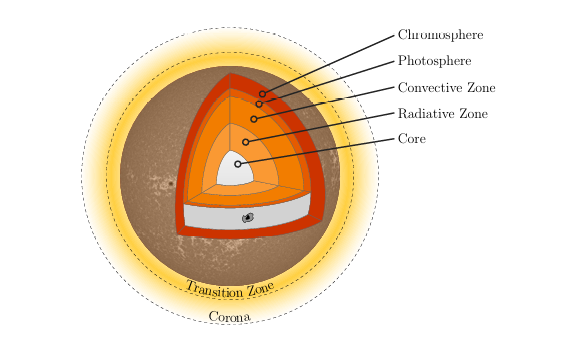
\includegraphics[height=0.6\textheight,width=\linewidth,keepaspectratio]{solar/sun_parts.png}\par
        \vspace{0.05cm}
        {\scriptsize Capas y regiones del Sol [4].}
        \column{0.49\textwidth}
        \centering
        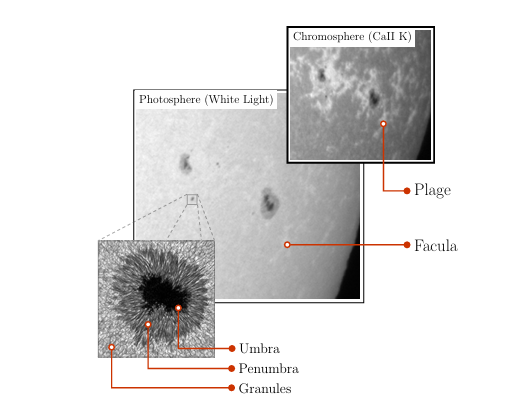
\includegraphics[height=0.6\textheight,width=\linewidth,keepaspectratio]{solar/wl_cak.png}\par
        \vspace{0.05cm}
        {\scriptsize Comparación luz blanca y CaII K [4].}
    \end{columns}
    
    \vfill
    {\tiny\color{gray} [4] M. Sayez et al., “SunSCC: Automated solar classification dataset” Astronomy \& Astrophysics, 2023.}
\end{frame}

\begin{frame}{Manchas Solares}
    \vspace{0.2cm} % Margen inicial sutil debajo del título del frame

    \centering % Centra el bloque completo de columnas respecto al ancho de la diapositiva
    \begin{columns}[c, onlytextwidth] % forces exact distribution across the text width
        
        % Columna IZQUIERDA: Disco solar completo
        \begin{column}{0.48\textwidth}
            \centering
            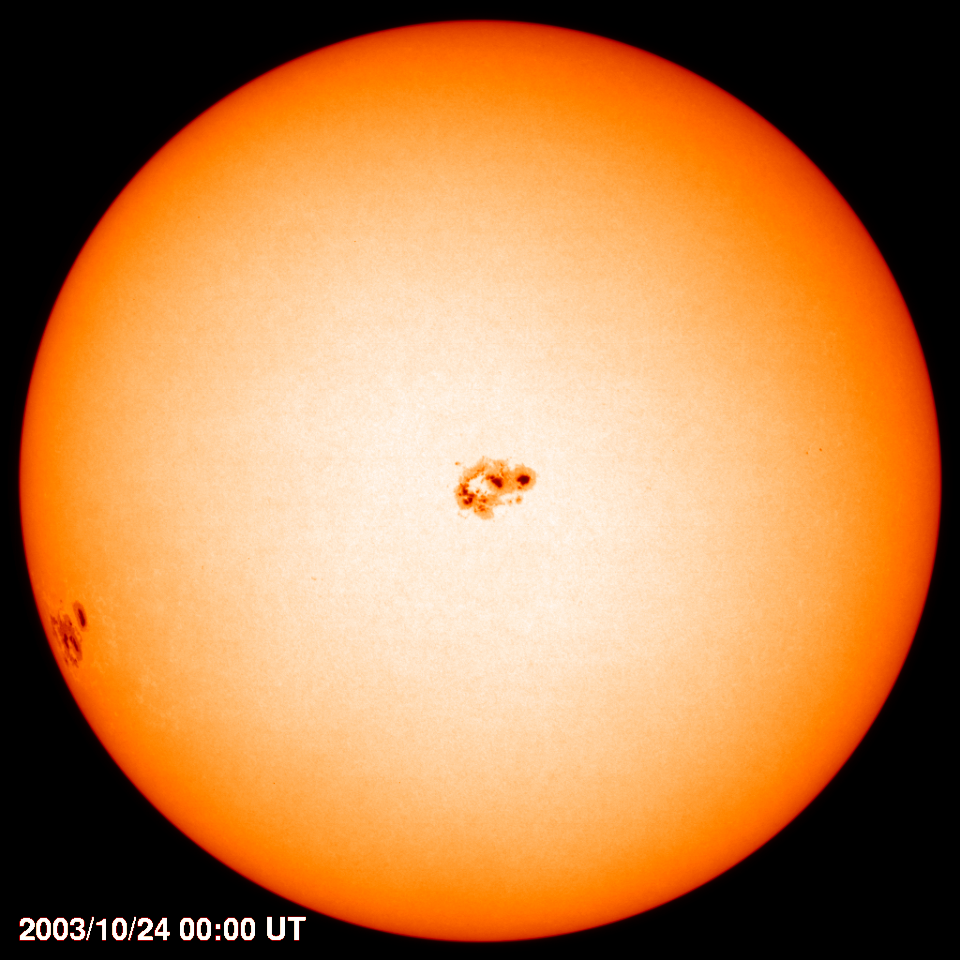
\includegraphics[height=0.55\textheight, width=\linewidth, keepaspectratio]{solar/sunspot.png}\par
            \vspace{0.08cm}
            {\scriptsize Disco solar completo [3].}
        \end{column}
        
        \hfill % Introduce un espacio elástico exacto en el medio para empujar las cosas a los extremos equilibrados
        
        % Columna DERECHA: Detalle ampliado
        \begin{column}{0.48\textwidth}
            \centering
            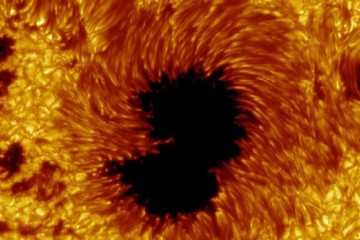
\includegraphics[height=0.55\textheight, width=\linewidth, keepaspectratio]{solar/spot_close.jpg}\par
            \vspace{0.08cm}
            {\scriptsize Detalle ampliado de una mancha solar [3].}
        \end{column}
        
    \end{columns}
    
    \vfill % Empuja la referencia estrictamente al límite inferior de la diapositiva

    % Bloque de Referencia a pie de página
    {\tiny\color{gray} [3] P. H. Scherrer et al., “The Helioseismic and Magnetic Imager (HMI) investigation on the Solar Dynamics Observatory (SDO),” \textit{Solar Physics}, vol. 275, pp. 207--227, 2012.}
\end{frame}

\begin{frame}{Sistemas de Clasificación de Manchas solares}
    \centering
    \begin{columns}
        \column{0.49\textwidth}
        \centering
        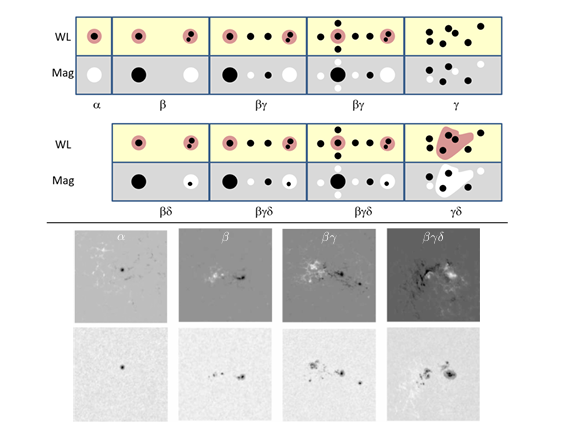
\includegraphics[height=0.6\textheight,width=\linewidth,keepaspectratio]{solar/wilson.png}\par
        \vspace{0.05cm}
        {\scriptsize Clasificación de Wilson (8 clases) [5].}
        \column{0.49\textwidth}
        \centering
        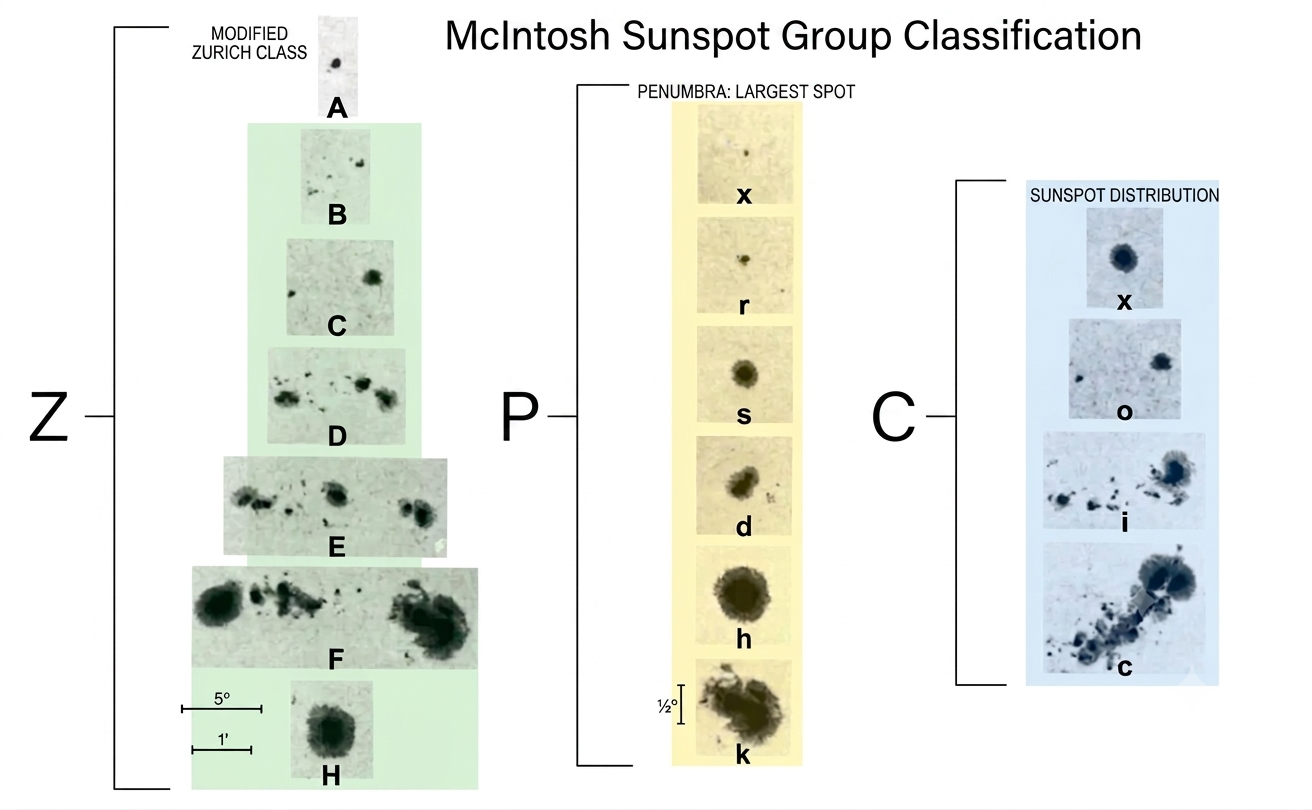
\includegraphics[height=0.6\textheight,width=\linewidth,keepaspectratio]{solar/mcintosh.png}\par
        \vspace{0.05cm}
        {\scriptsize Clasificación de Zürich--McIntosh (60 clases) [5].}
    \end{columns}\par
    
    \vfill
    {\tiny\color{gray} [5] P. S. McIntosh, “The classification of sunspot groups,” Solar Physics, vol. 125, no. 2, pp. 251--267, 1990.\par}
\end{frame}

\begin{frame}{Observatorios Terrestres y Contexto Local}
    \centering
    \begin{columns}
        \column{0.32\textwidth}
        \centering
        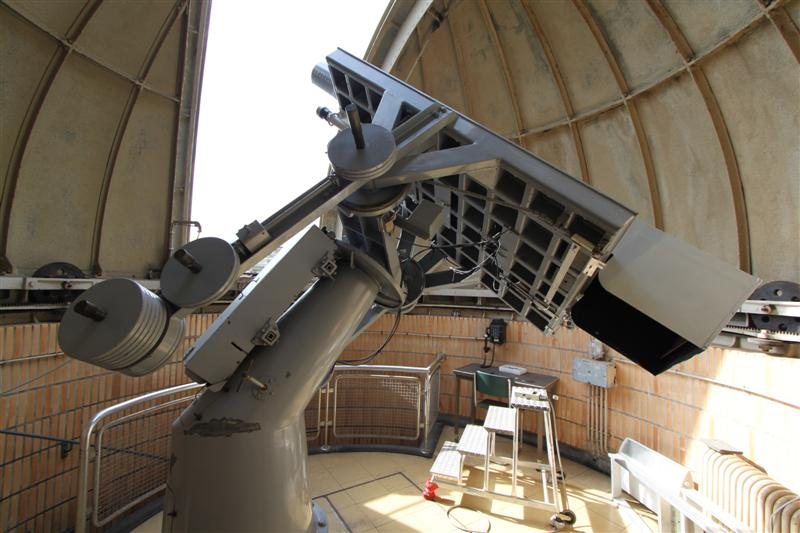
\includegraphics[height=0.46\textheight,width=\linewidth,keepaspectratio]{solar/scope_proj.jpg}\par
        \vspace{0.05cm}
        {\scriptsize Plataforma USET [6].}
        \column{0.32\textwidth}
        \centering
        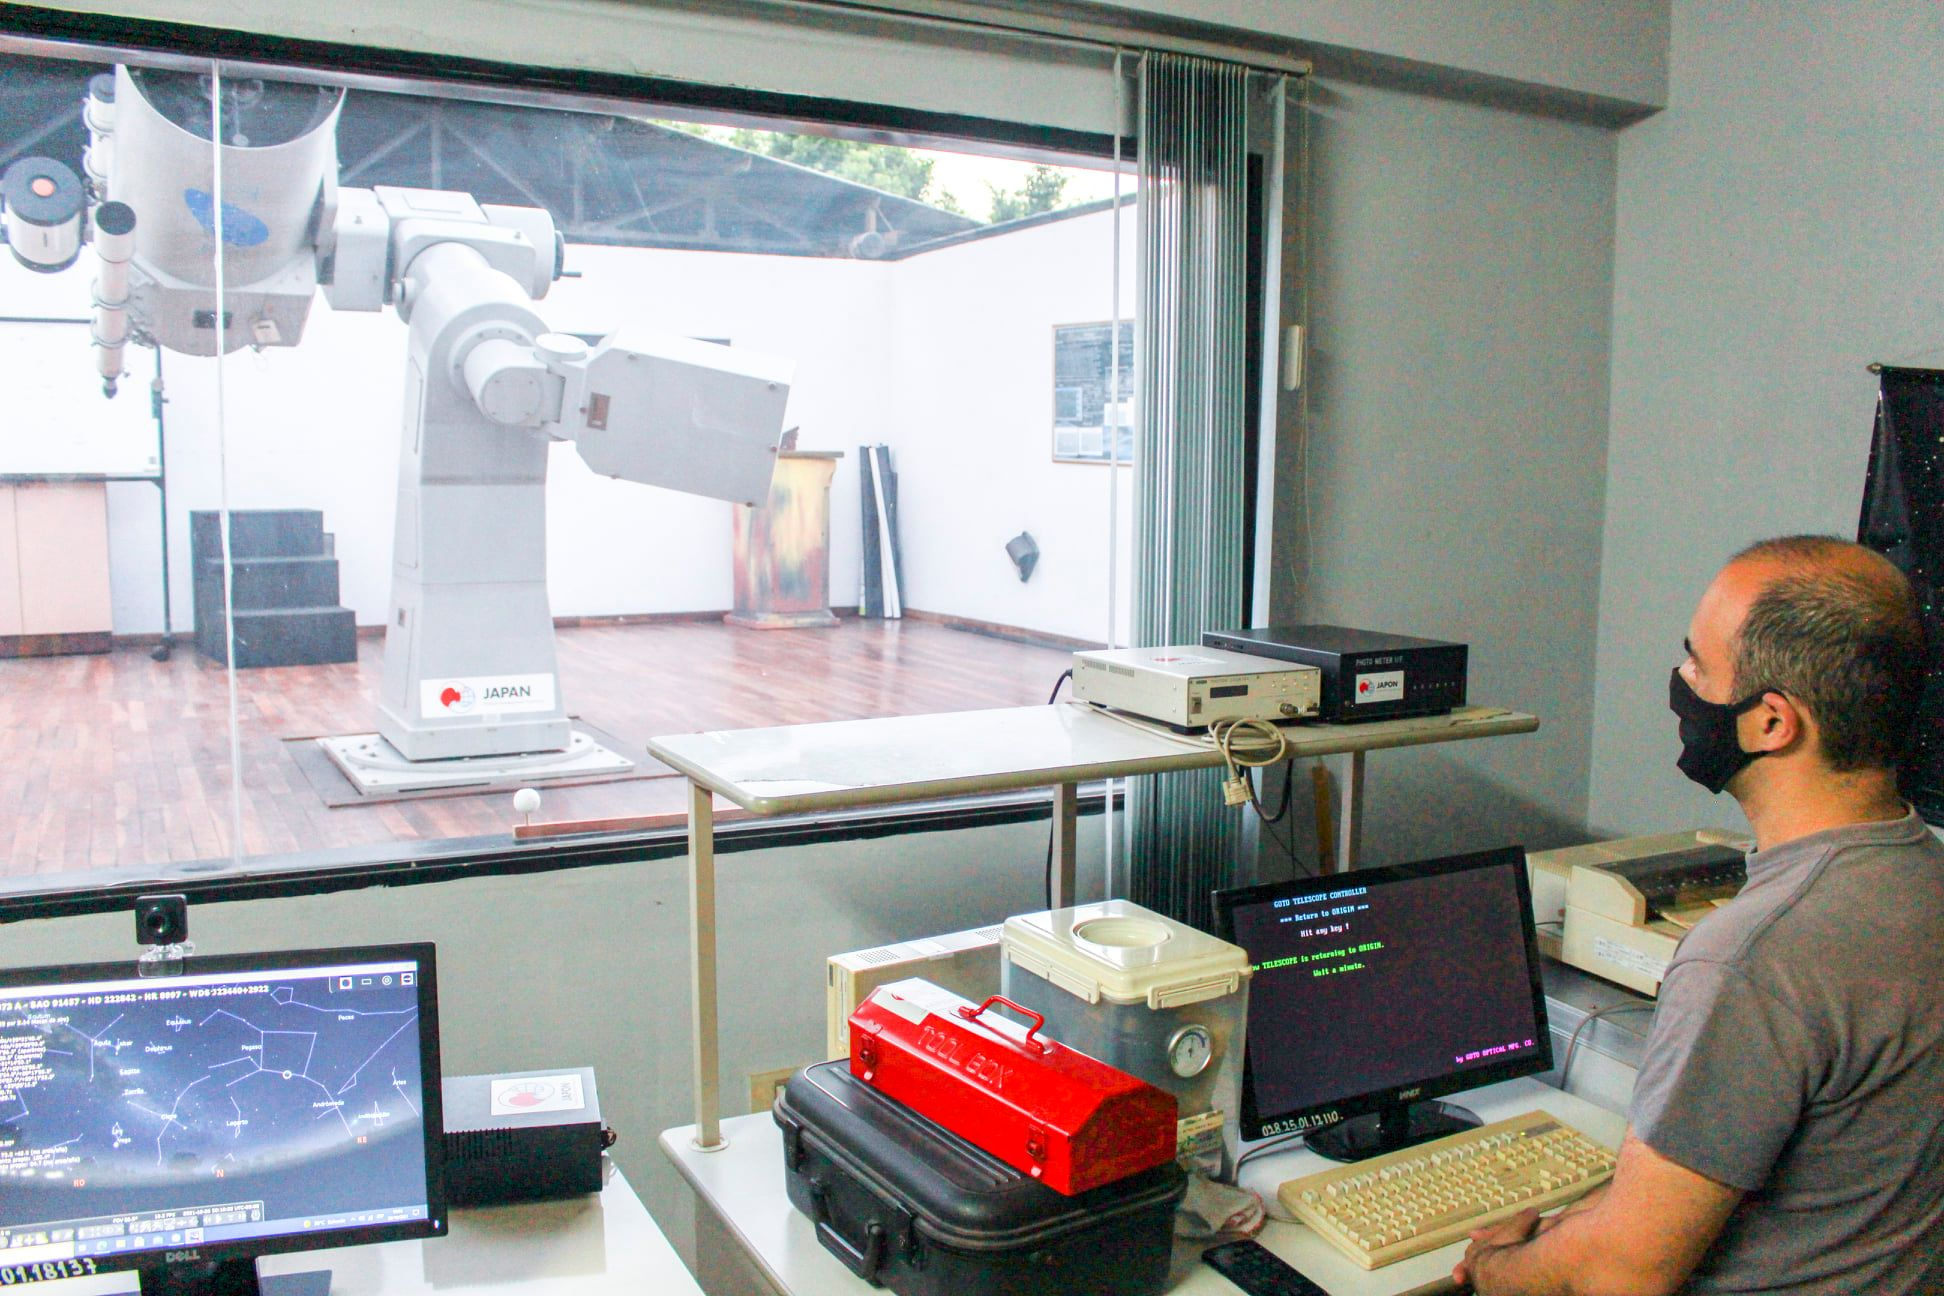
\includegraphics[height=0.46\textheight,width=\linewidth,keepaspectratio]{obs/control.jpg}\par
        \vspace{0.05cm}
        {\scriptsize Sala de control del observatorio "Prof. Alexis Troche Boggino".}
        \column{0.32\textwidth}
        \centering
        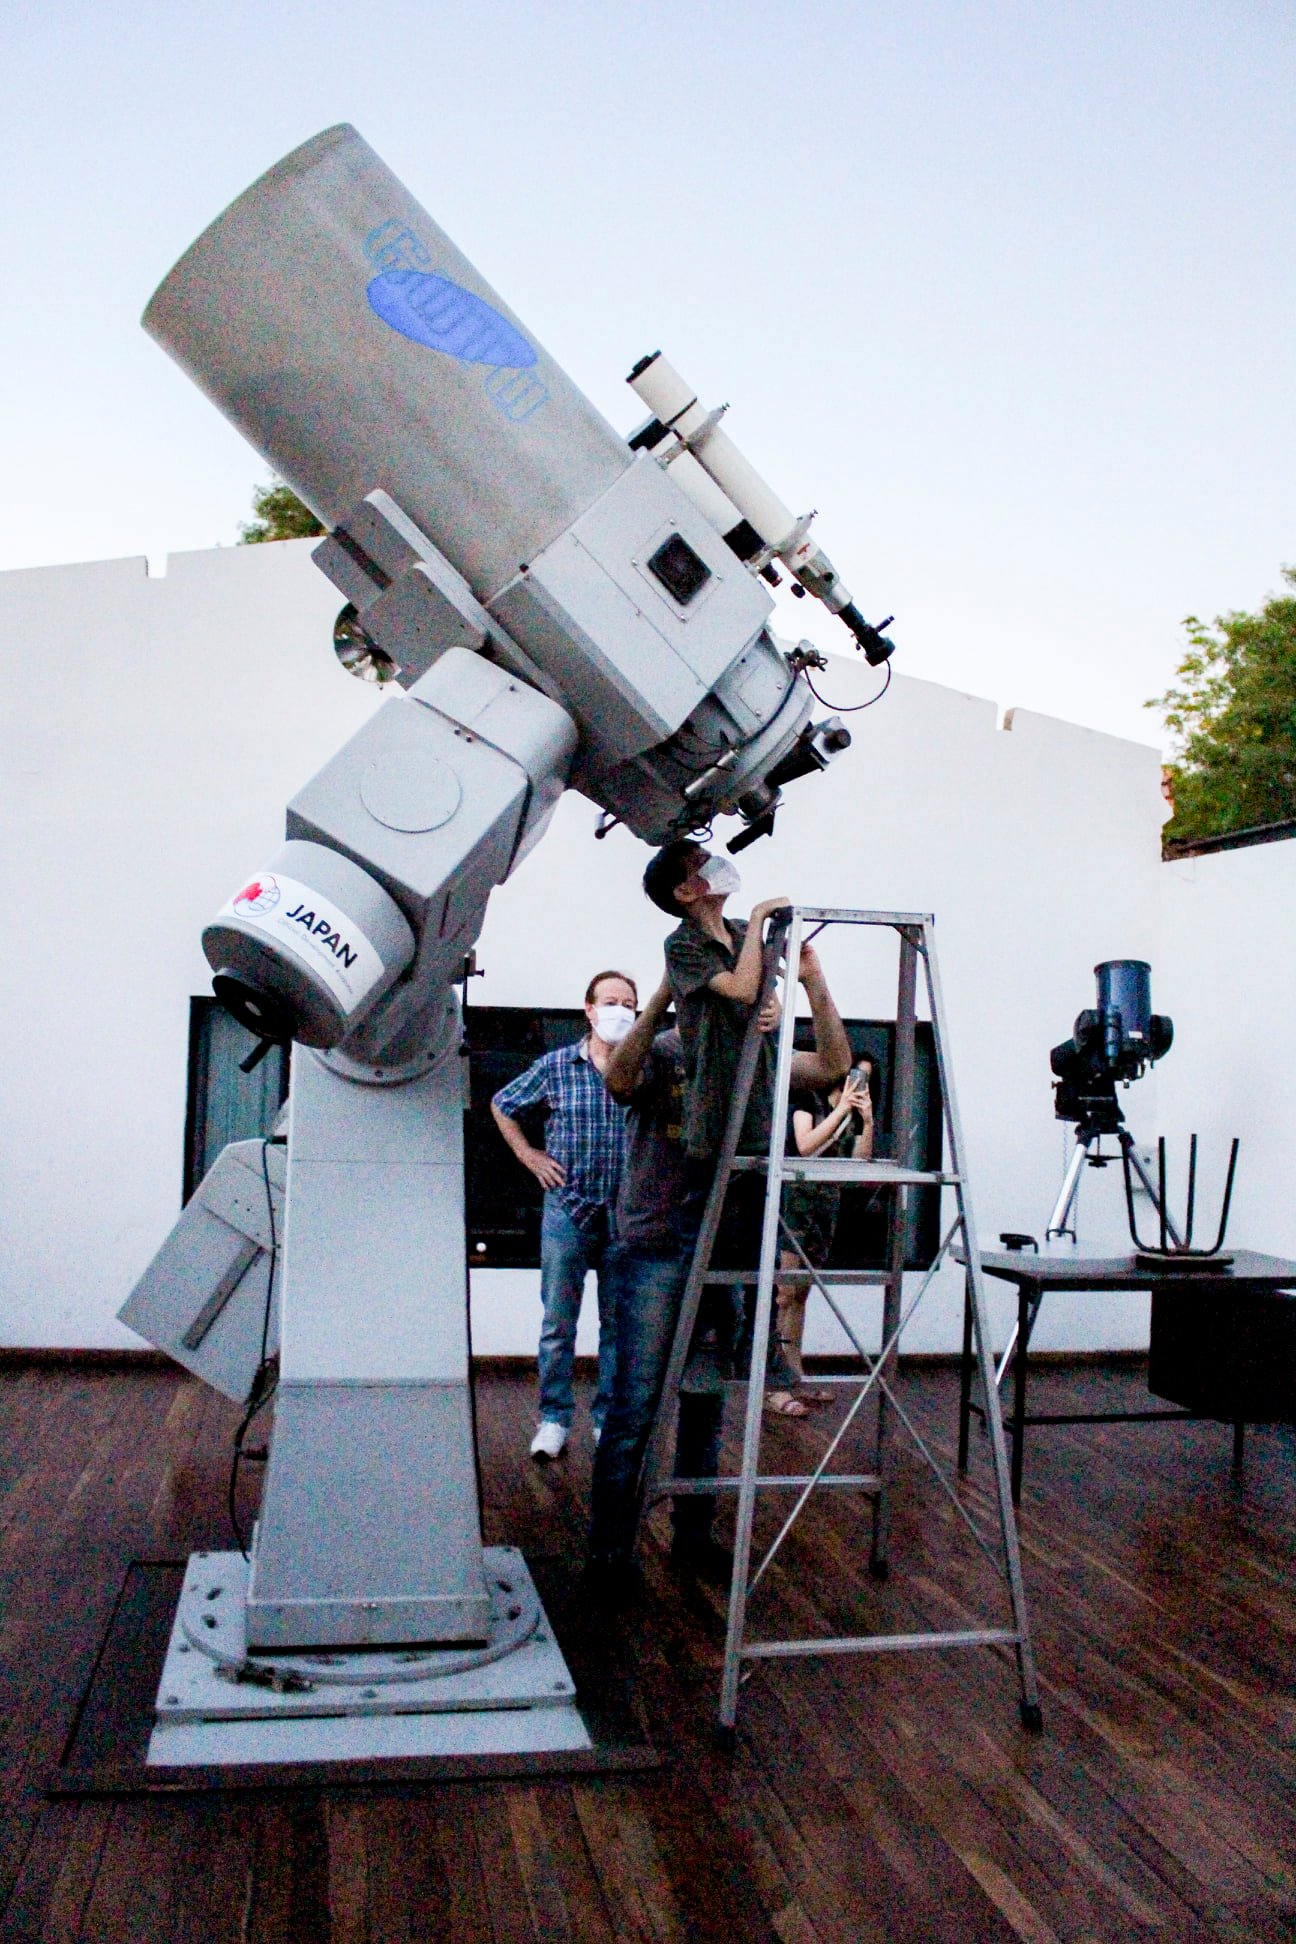
\includegraphics[height=0.46\textheight,width=\linewidth,keepaspectratio]{obs/scope.jpg}\par
        \vspace{0.05cm}
        {\scriptsize Telescopio del Observatorio "Prof. Alexis Troche Boggino".}
    \end{columns}
    
    \vfill
    {\tiny\color{gray} [6] Royal Observatory of Belgium, “Understanding Solar Activity Telescopes (USET) report,” 2026.}
\end{frame}

\begin{frame}{Ciclo Solar}
    \centering
    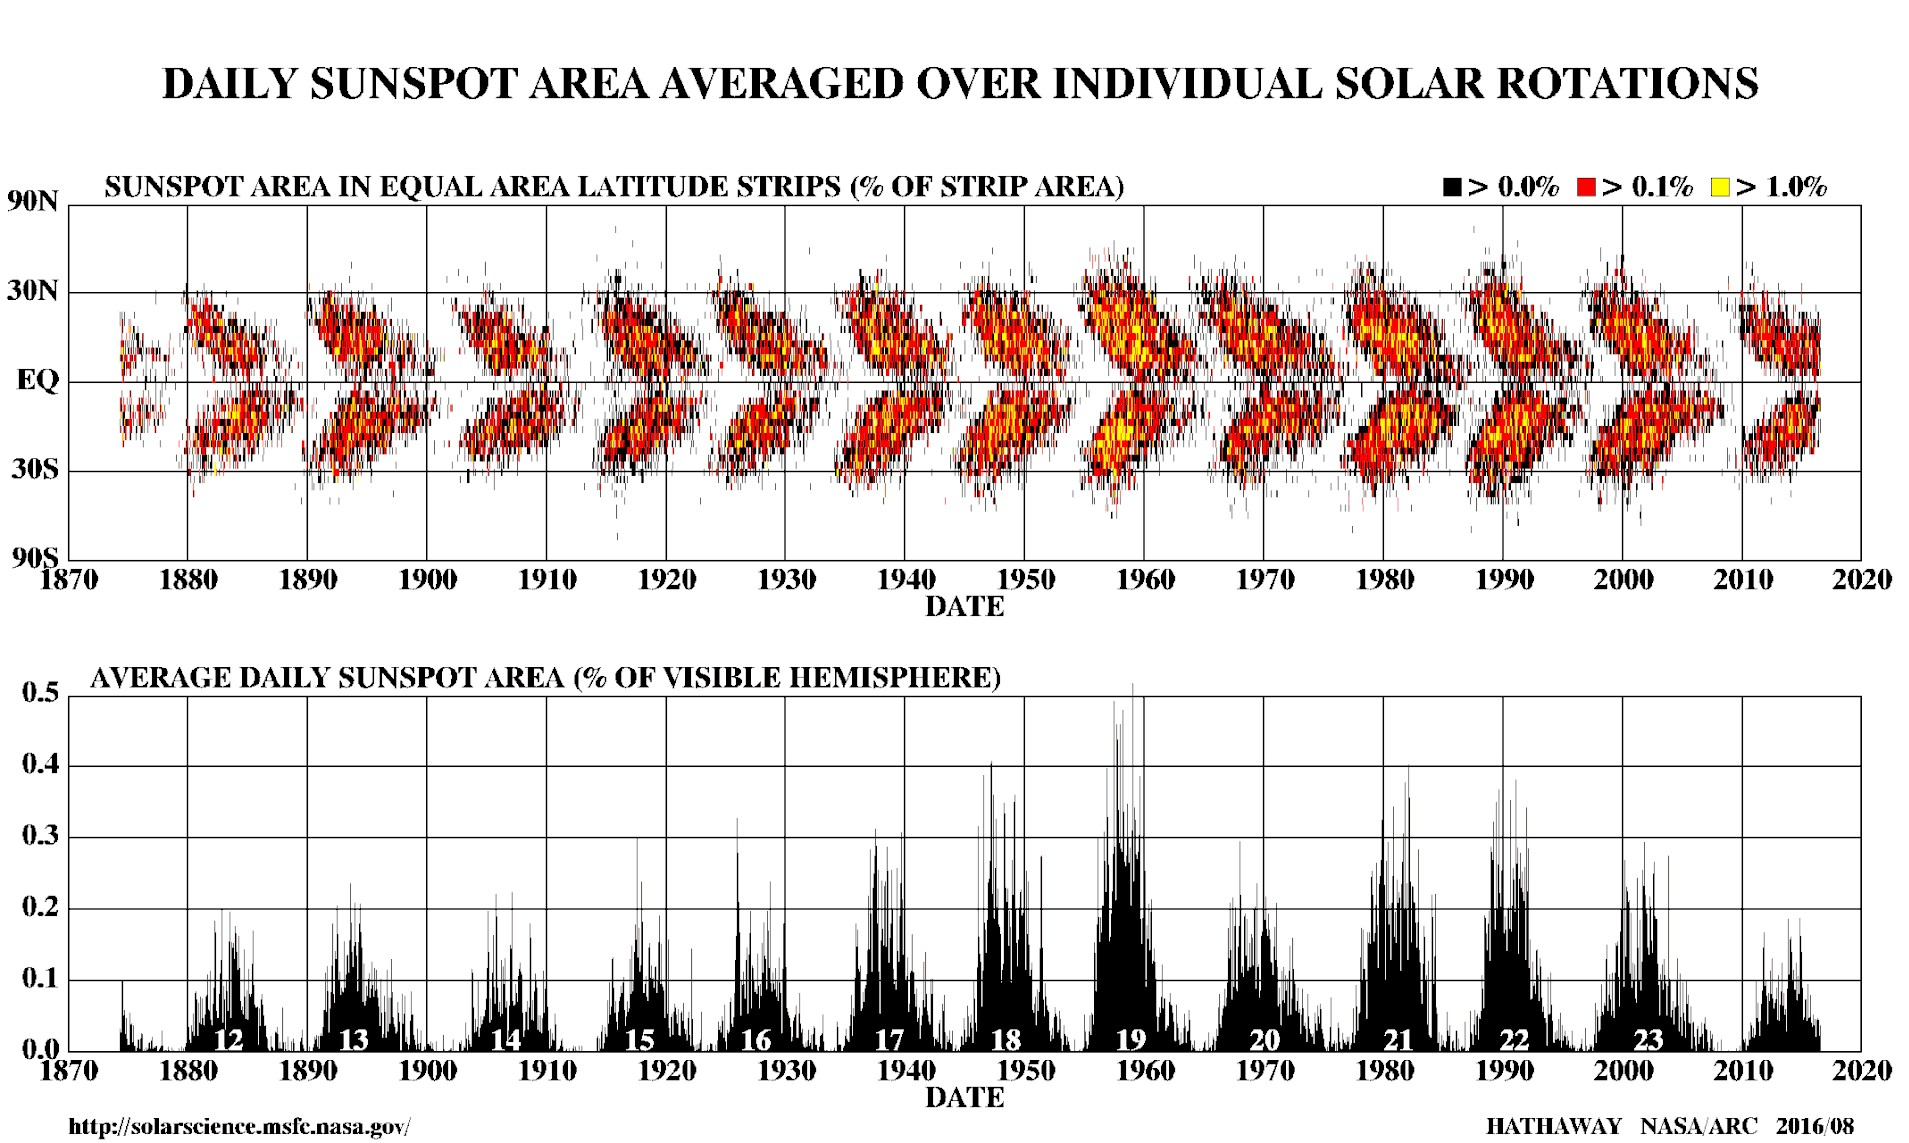
\includegraphics[height=0.62\textheight,width=0.96\linewidth,keepaspectratio]{solar/butterfly.jpg}\par
    \vspace{0.05cm}
    {\scriptsize Diagrama de Spörer histórico [7].}
    
    \vfill
    {\tiny\color{gray} [7] D. H. Hathaway, “The solar cycle,” Living Reviews in Solar Physics, vol. 12, no. 1, pp. 1--70, 2015.}
\end{frame}


\section{Estado del Arte}

% \begin{frame}{Estado del Arte: Contexto y Brecha Tecnológica}
%     \begin{block}{La Brecha en el Mercado Actual}
%         En la actualidad, \textbf{no existen ecosistemas comerciales} de observación astrofotográfica que integren de extremo a extremo todo el flujo de trabajo científico:
%     \end{block}

%     \vspace{0.3cm}
%     \begin{columns}[T]
%         \column{0.45\textwidth}
%         \centering
%         \textbf{Flujo Comercial Convencional}
%         \vspace{0.2cm}
%         \begin{itemize}
%             \item Adquisición asistida aislada.
%             \item Dependencia de software de terceros.
%             \item Sin análisis científico local.
%         \end{itemize}

%         \column{0.10\textwidth}
%         \centering
%         \vspace{0.6cm}
%         $\mathbf{\Longrightarrow}$

%         \column{0.45\textwidth}
%         \centering
%         \textbf{Propuesta del Prototipo}
%         \vspace{0.2cm}
%         \begin{itemize}
%             \item \color{deepblue} Captura + Preprocesamiento local.
%             \item \color{deepblue} Inferencia por IA en cascada.
%             \item \color{deepblue} Modelos predictivos del ciclo solar.
%         \end{itemize}
%     \end{columns}

%     \vspace{0.4cm}
%     \centering
%     \small \textit{Por lo tanto, el estado del arte se analiza bajo las siguientes dimensiones críticas:}
% \end{frame}

% \begin{frame}{Dispositivos comerciales de adquisición asistida}
%     \begin{columns}
%         \column{0.32\textwidth}
%         \centering
%         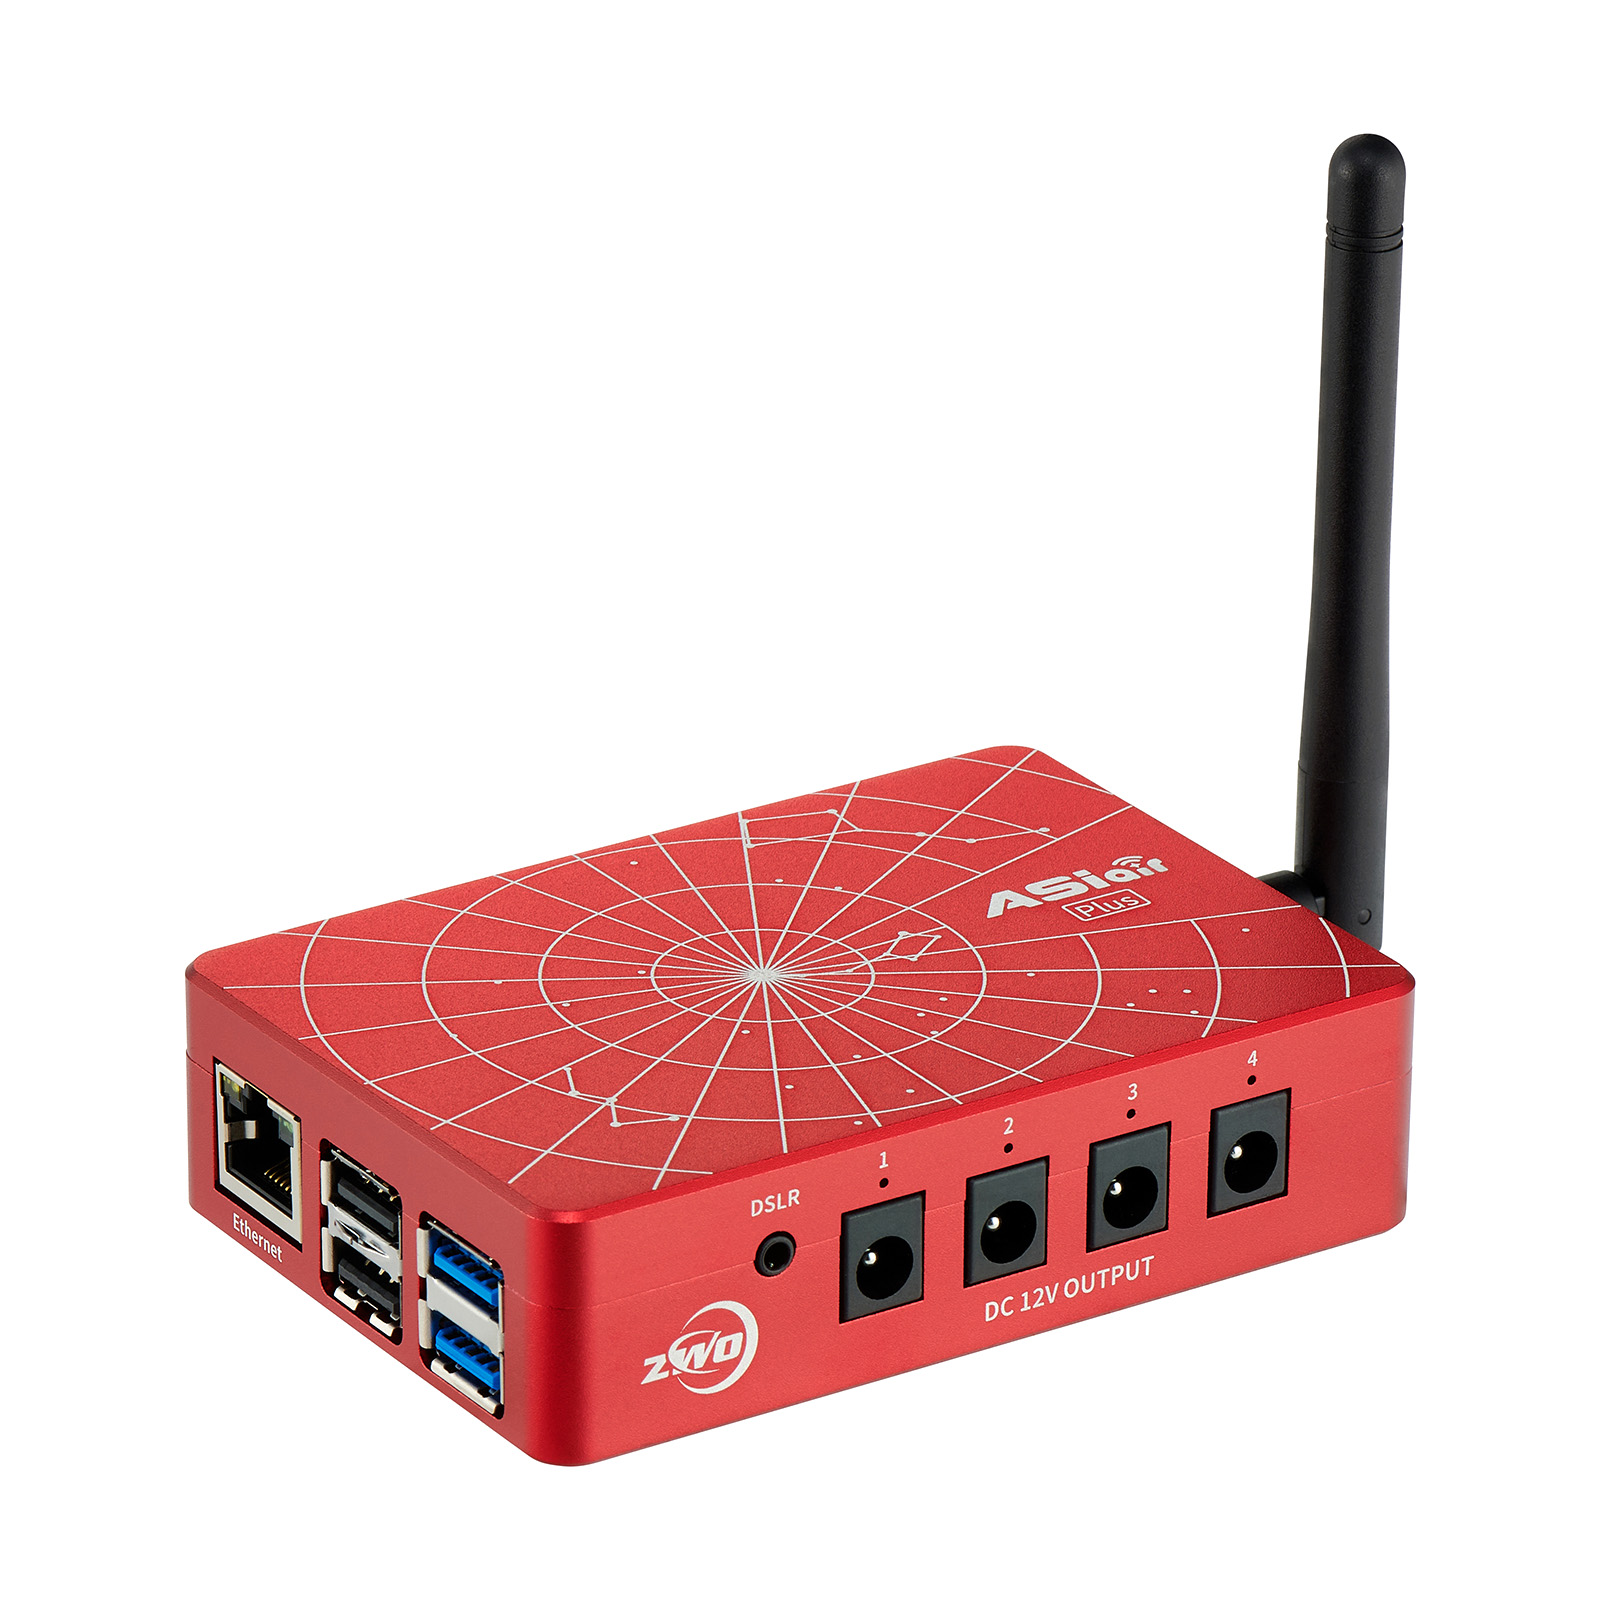
\includegraphics[height=0.50\textheight,width=\linewidth,keepaspectratio]{hw_art_state/zwo_asiair.jpg}\par
%         \vspace{0.03cm}
%         {\scriptsize ZWO ASIAIR [8].}
%         \column{0.32\textwidth}
%         \centering
%         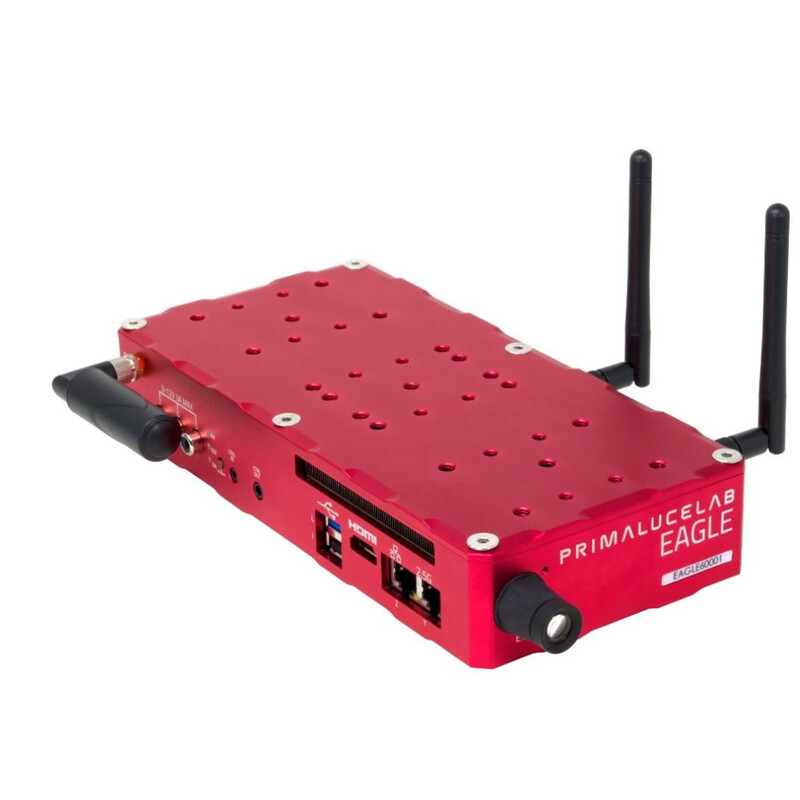
\includegraphics[height=0.50\textheight,width=\linewidth,keepaspectratio]{hw_art_state/primaLuceLab-Eagle6.jpg}\par
%         \vspace{0.03cm}
%         {\scriptsize PrimaLuceLab EAGLE6 [8].}
%         \column{0.32\textwidth}
%         \centering
%         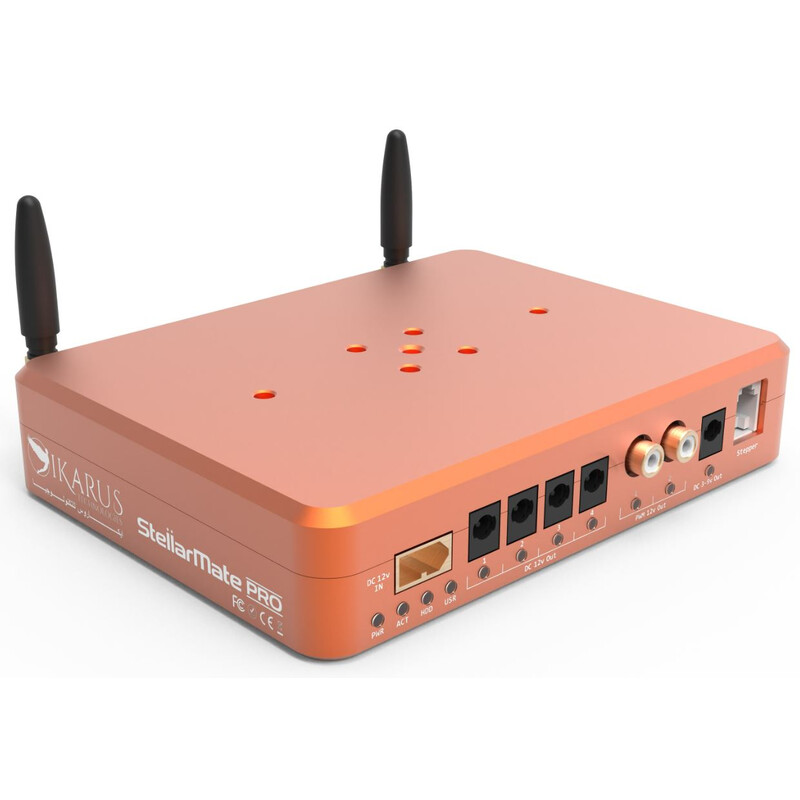
\includegraphics[height=0.50\textheight,width=\linewidth,keepaspectratio]{hw_art_state/stellar_mate-pro-8GB-128GB.jpg}\par
%         \vspace{0.03cm}
%         {\scriptsize StellarMate Pro [8].}
%     \end{columns}
    
%     \vfill
%     {\tiny\color{gray} [8] ZWO Optical Inc., “ASI Cameras Product Manual and Technical Integration Specifications,” v4.2, 2025.}
% \end{frame}

% \begin{frame}{Comparación de hardware comercial}
%     \centering
%     \circle
%     \small
%     \begin{table}
%         \centering
%         \setlength{\tabcolsep}{4pt}
%         \begin{tabular}{ll}
%             \toprule
%             \textbf{Sistema} & \textbf{Síntesis} \\
%             \midrule
%             ASIAIR & captura asistida, ecosistema cerrado, costo bajo--medio \\
%             EAGLE6 & PC astronómico robusto, múltiples puertos, costo alto \\
%             StellarMate & plataforma Linux abierta, automatización, costo medio \\
%             Prototipo & captura, registro, IA y predicción en flujo académico \\
%             \bottomrule
%         \end{tabular}
%     \end{table}
% \end{frame}

\begin{frame}{Referencias Modernas de Detección y Clasificación}
    \centering
    
    \begin{columns}
        \column{0.49\textwidth}
        \centering
        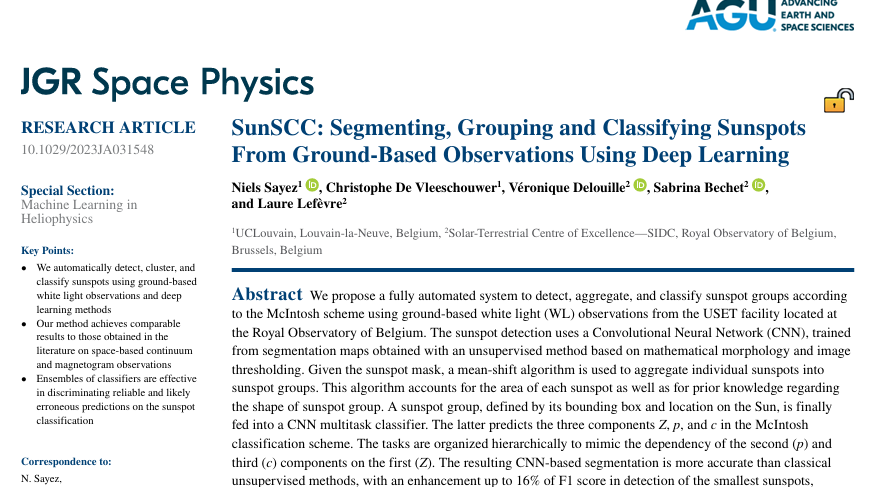
\includegraphics[height=0.62\textheight,width=\linewidth,keepaspectratio]{ref/etSayez.png}\par
        \vspace{0.03cm}
        {\scriptsize Article SunSCC--Automated solar classification dataset [4].}
        \column{0.49\textwidth}
        \centering
        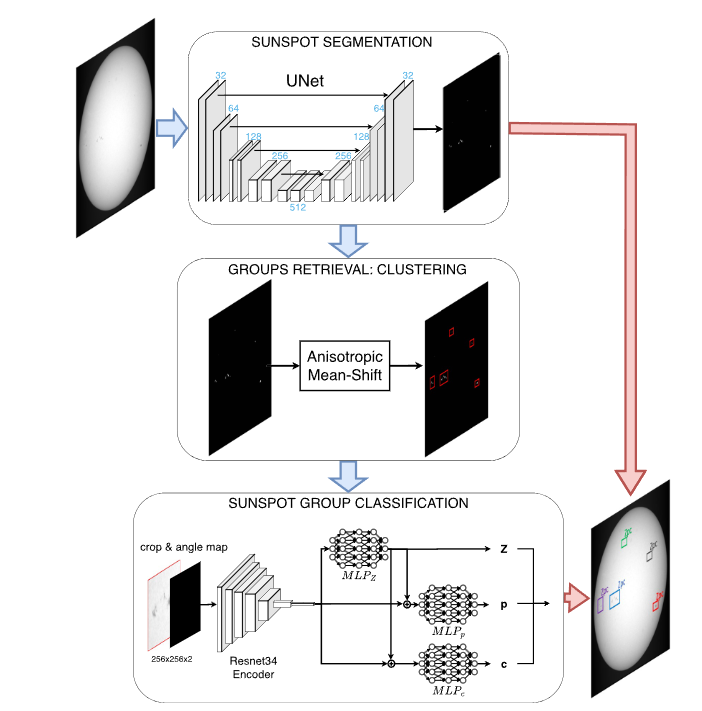
\includegraphics[height=0.6\textheight,width=\linewidth,keepaspectratio]{ml/yolo_train.png}\par
        \vspace{0.03cm}
        {\scriptsize Arquitectura modular de segmentacion, deteccion y clasificacion [4].}
    \end{columns}
    
    \vfill
    {\tiny\color{gray} [4] M. Sayez et al., “SunSCC: Automated solar classification dataset,” Astronomy \& Astrophysics, 2023.}
\end{frame}

\begin{frame}{YOLO26--Etapa de Detección}
    \centering
    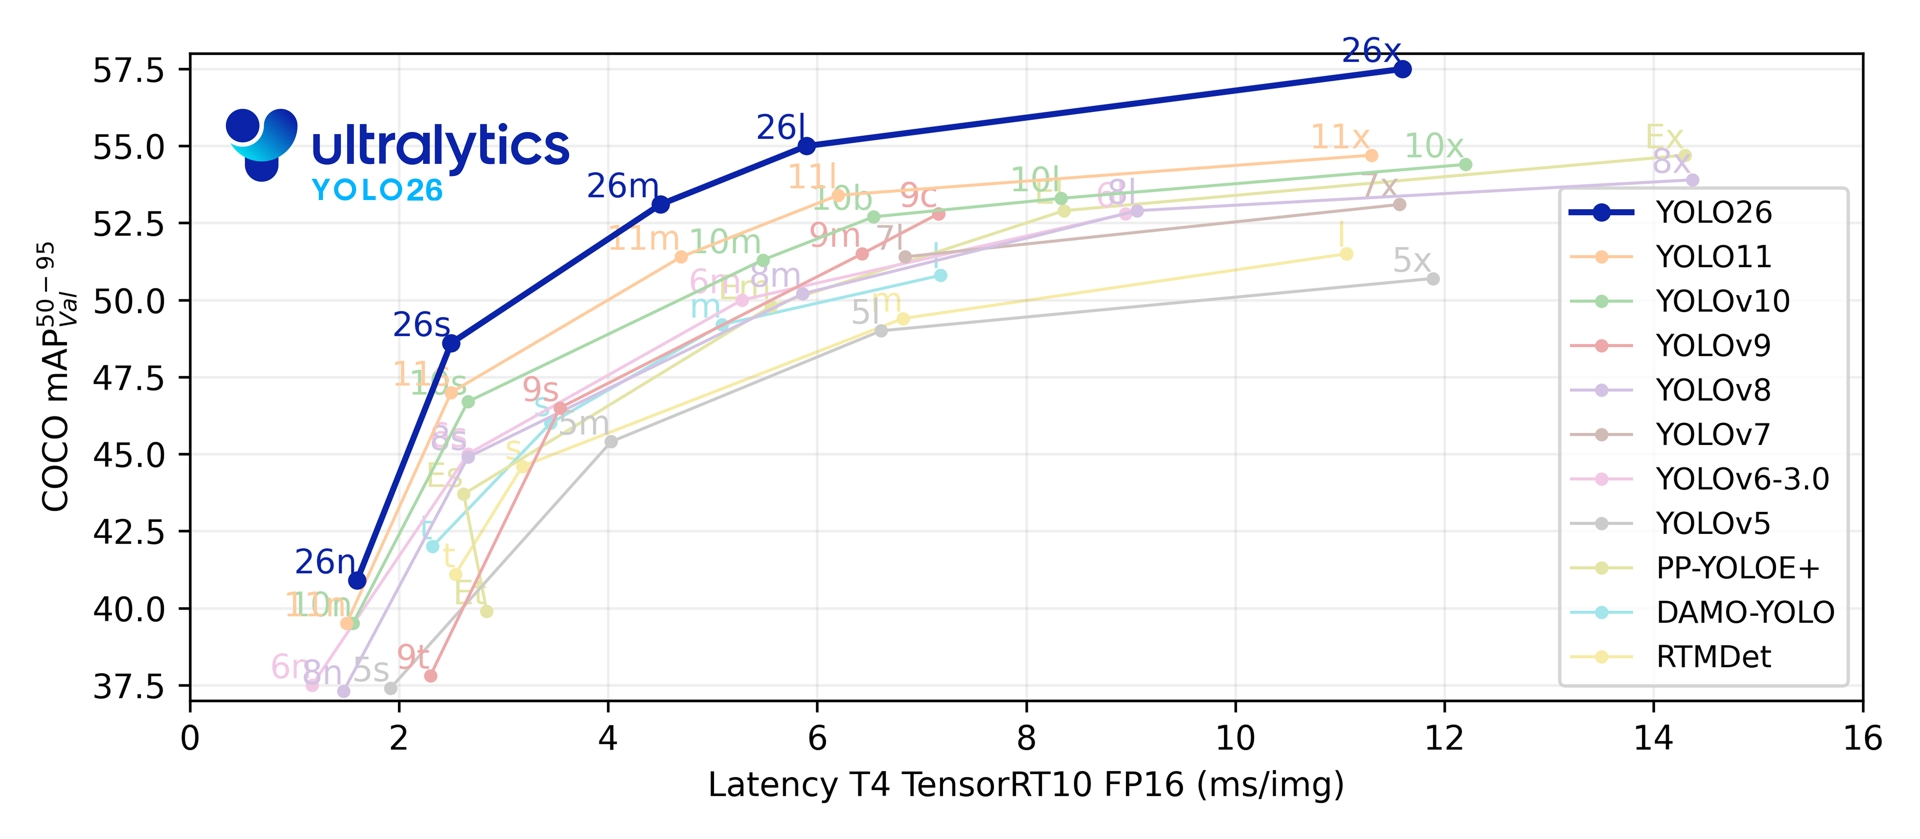
\includegraphics[height=0.62\textheight,width=0.96\linewidth,keepaspectratio]{ml/yolo_bench.jpg}\par
    \vspace{0.05cm}
    {\scriptsize Comparación de rendimiento de la familia YOLO [8].}
    
    \vfill
    {\tiny\color{gray} [8] Ultralytics LLC, “YOLO26 Real-Time Object Detection Engine and Benchmarks,” 2026.}
\end{frame}

\begin{frame}{ConvNeXtV2--Etapa de Clasificación}
    \begin{columns}
        \column{0.49\textwidth}
        \centering
        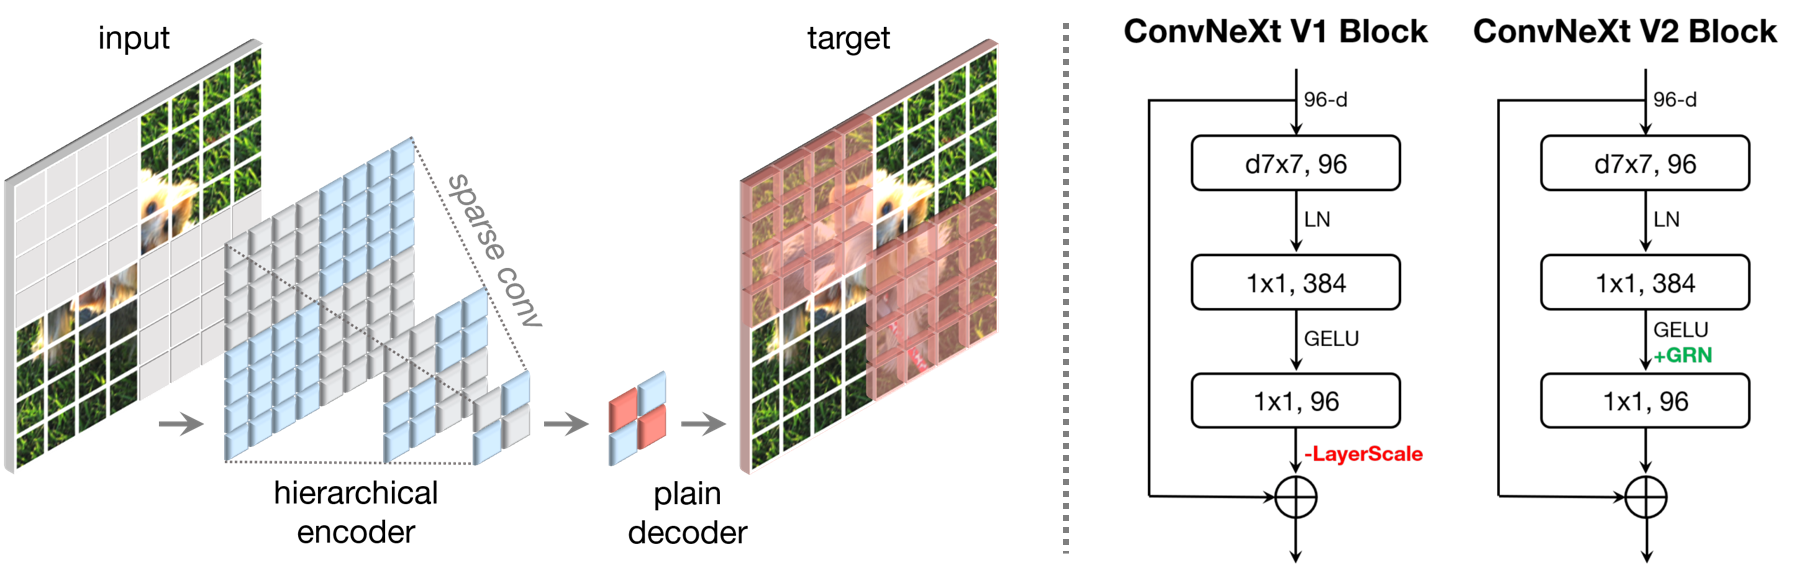
\includegraphics[height=0.54\textheight,width=\linewidth,keepaspectratio]{ml/fcmae.png}\par
        \vspace{0.03cm}
        {\scriptsize Preentrenamiento FCMAE [10].}
        \column{0.49\textwidth}
        \centering
        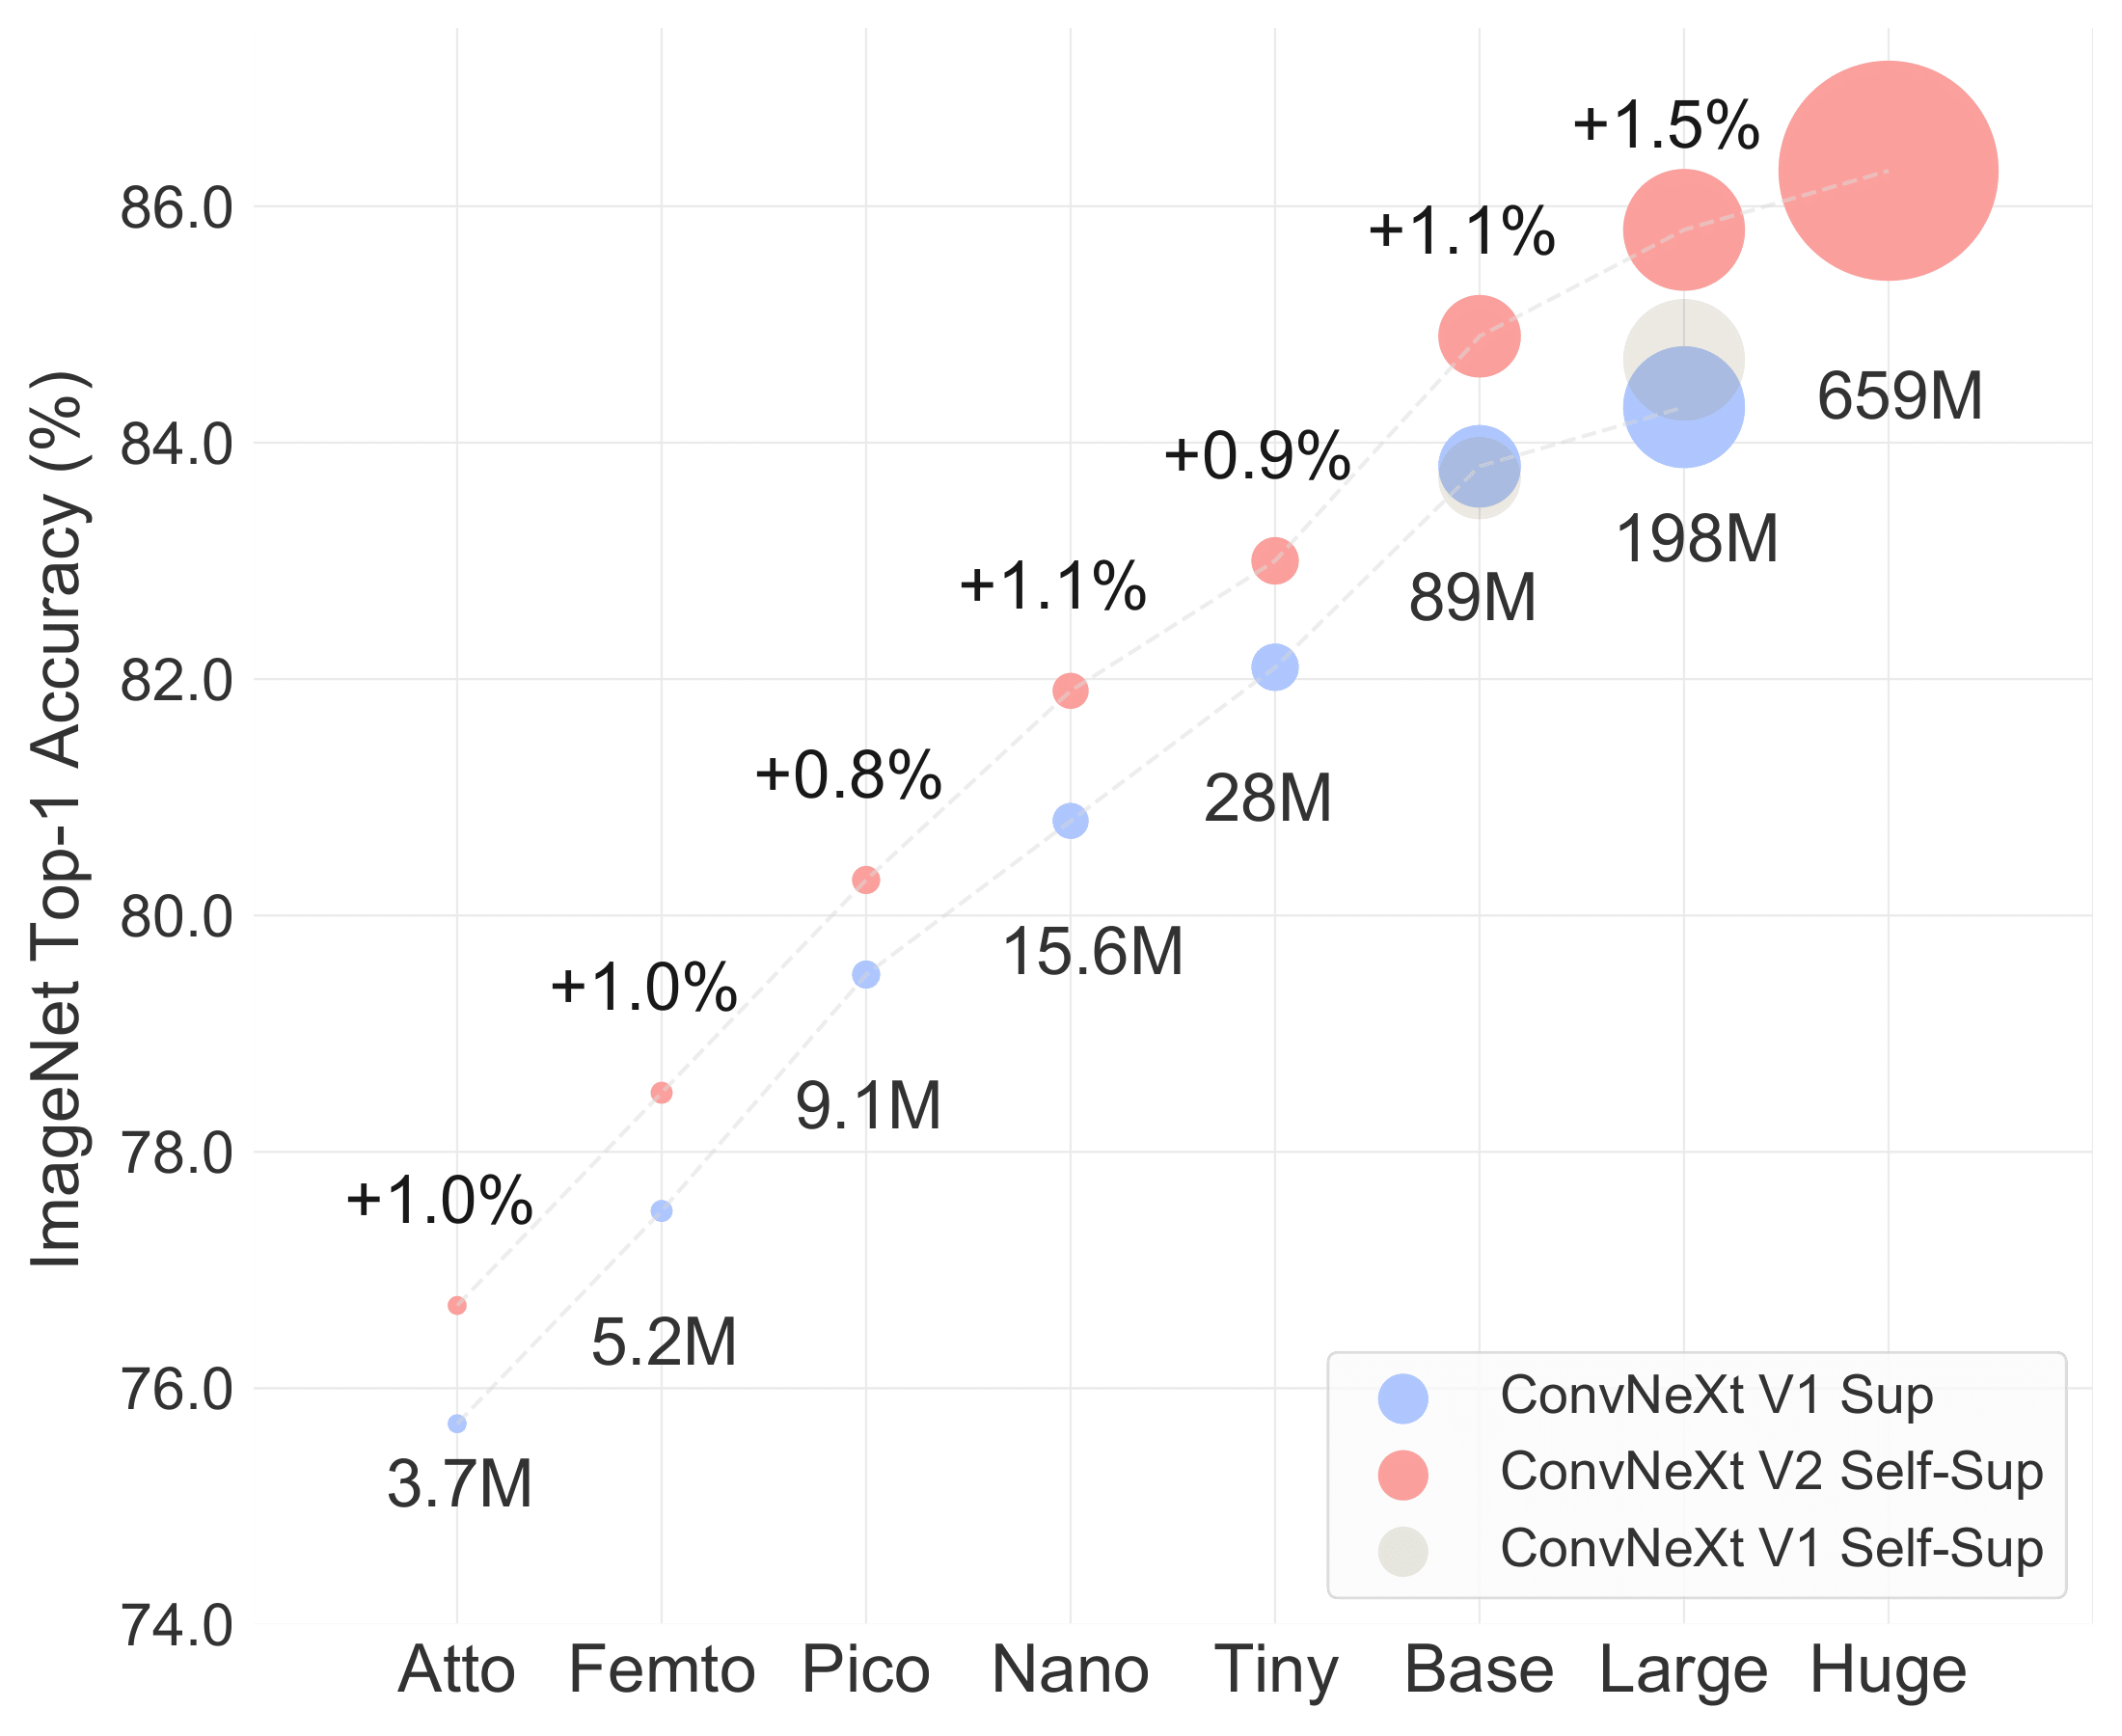
\includegraphics[height=0.54\textheight,width=\linewidth,keepaspectratio]{ml/scaling.png}\par
        \vspace{0.03cm}
        {\scriptsize Escalamiento ConvNeXtV2 [10].}
    \end{columns}
    
    \vfill
    {\tiny\color{gray} [10] S. Woo et al., “ConvNeXt V2: Co-designing and scaling convnets with masked autoencoders,” in Proc. IEEE/CVF CVPR, 2023, pp. 16133--16142.}
\end{frame}

\begin{frame}{Modelos Predictivos}
    \vspace{0.1cm}

    \begin{columns}[c, onlytextwidth]
        \begin{column}{0.48\textwidth}
            \centering
            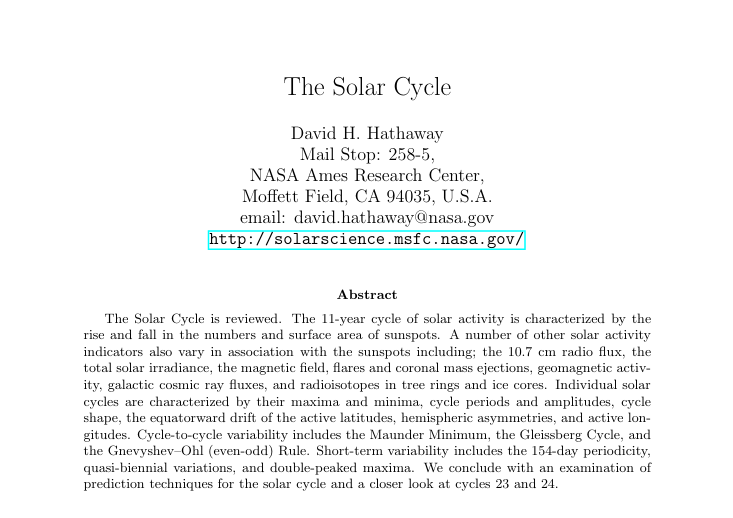
\includegraphics[height=0.55\textheight,width=\linewidth,keepaspectratio]{ref/etHathaway.png}\par
            \vspace{0.05cm}
            {\scriptsize Article The Solar Cycle [7].}
        \end{column}
        
        \hfill
        
        \begin{column}{0.48\textwidth}
            \centering
            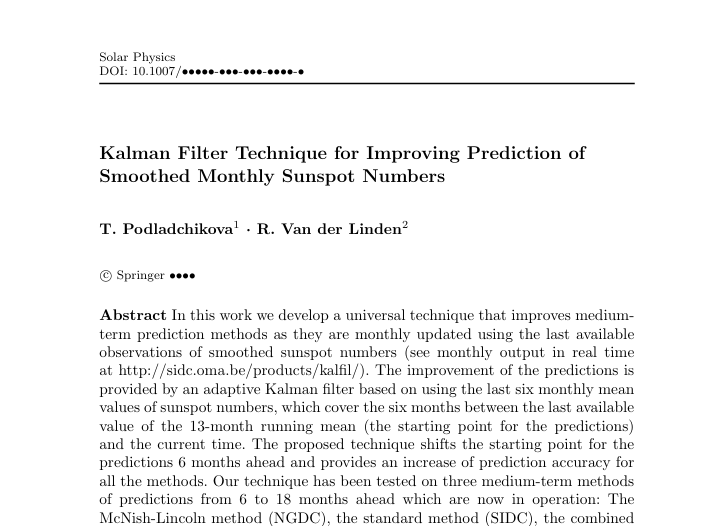
\includegraphics[height=0.55\textheight,width=\linewidth,keepaspectratio]{ref/etPLV.png}\par
            \vspace{0.05cm}
            {\scriptsize Article Kalman Filter Technique for SSN Improving Prediction [11].}
        \end{column}
    \end{columns}

    \vfill

    % Al agrupar todo dentro de un mismo bloque { }, el interlineado de tiny se aplica a todo el conjunto
    {\tiny\color{gray} 
    [7] D. H. Hathaway, “The solar cycle,” Living Reviews in Solar Physics, vol. 12, no. 1, pp. 1--70, 2015. \par\vspace{0.05cm}
    [11] Podladchikova, T. y Van der Linden, R. (2011). Kalman Filter Technique for Improving Prediction of Smoothed Monthly Sunspot Numbers. Solar Physics, 271(2), 469–485.\par}
\end{frame}

\section{Diseño de Hardware}

\begin{frame}{Módulo de Observación}
    \vspace{-0.4cm} % Sube el recuadro para que quede alineado con el título
    
    % Envuelve el cuadro y lo empuja hacia el extremo derecho exacto
    \begin{columns}[t]
        \begin{column}{\textwidth}
            \hfill
            \setlength{\fboxrule}{1.2pt} % Grosor del borde
            \setlength{\fboxsep}{4pt}    % Margen interno del cuadro
            \fcolorbox{llamativoMagenta}{white}{%
                \scriptsize\textcolor{llamativoMagenta}{\textbf{Contribución 1}}
            }
        \end{column}
    \end{columns}
    
    %\vspace{-0.2cm} % Compensa el espacio vertical para no empujar la imagen hacia abajo
    
    % --- CONTENIDO PRINCIPAL ---
    \centering
    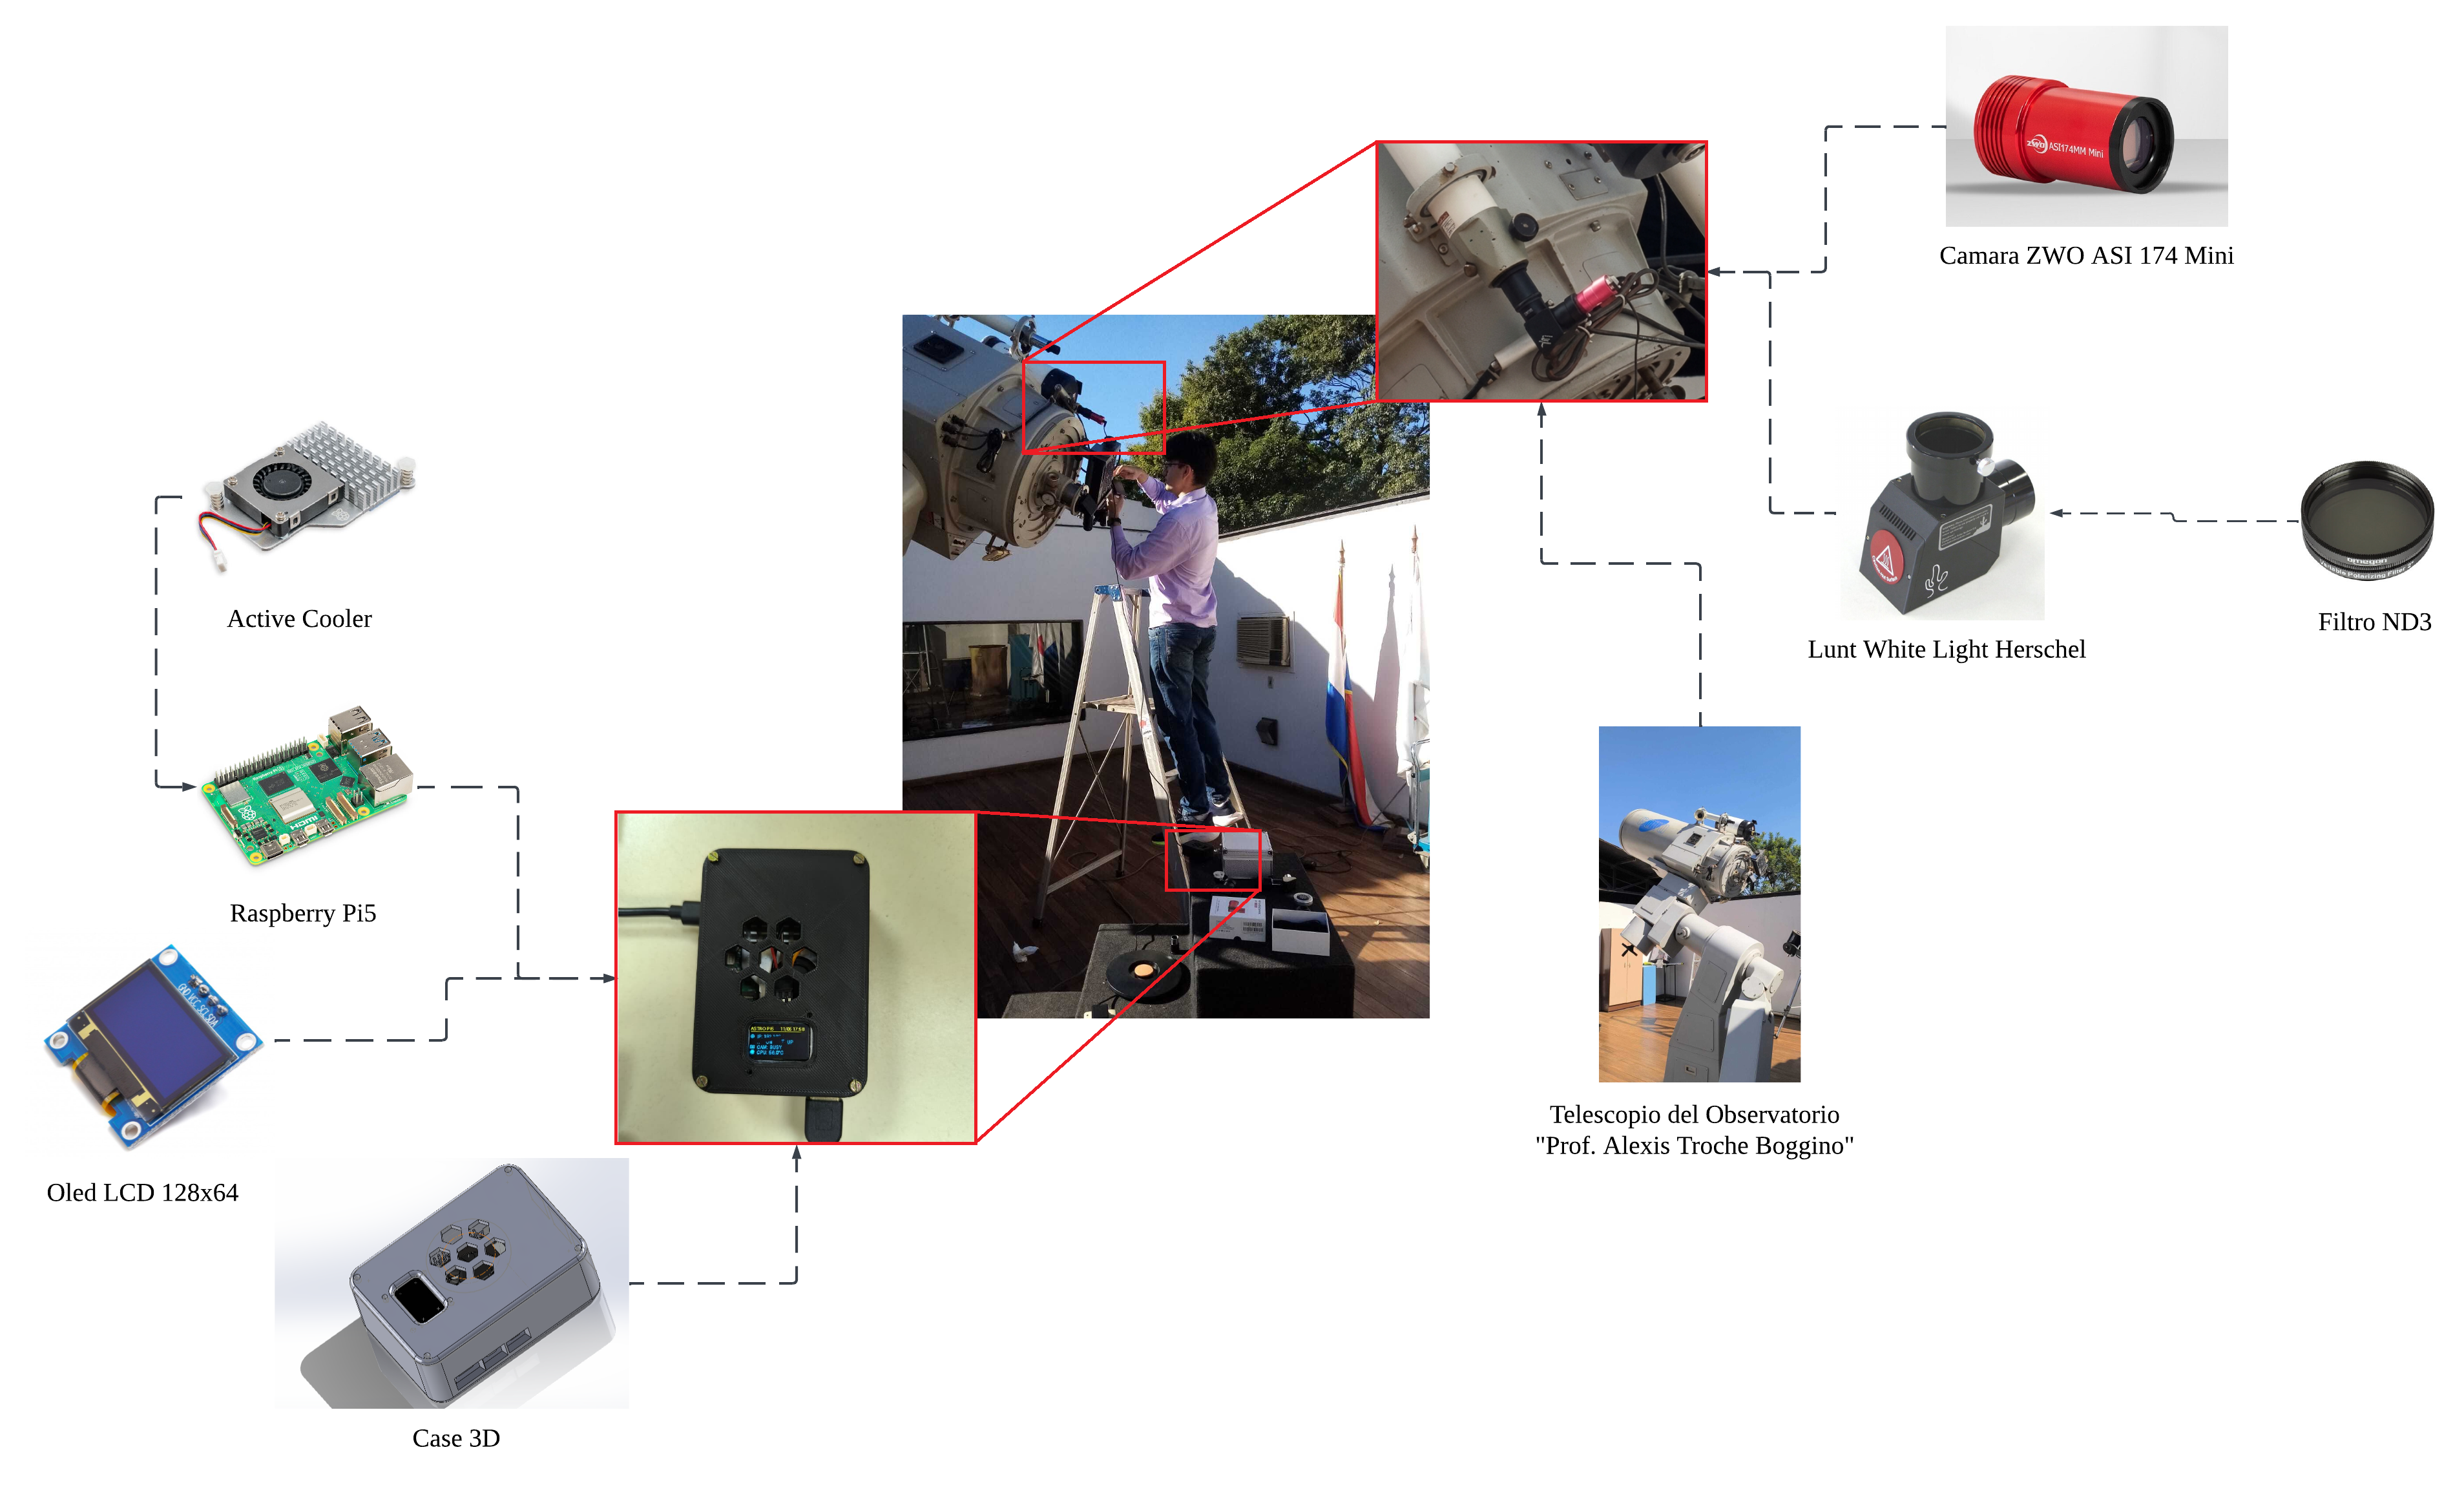
\includegraphics[height=0.85\textheight, width=0.96\linewidth, keepaspectratio]{hw/hw_diagram.png}
    \vspace{0.08cm}
\end{frame}



% \begin{frame}{Selección de Componentes}
%     \begin{columns}
%         \column{0.48\textwidth}
%         \centering
%         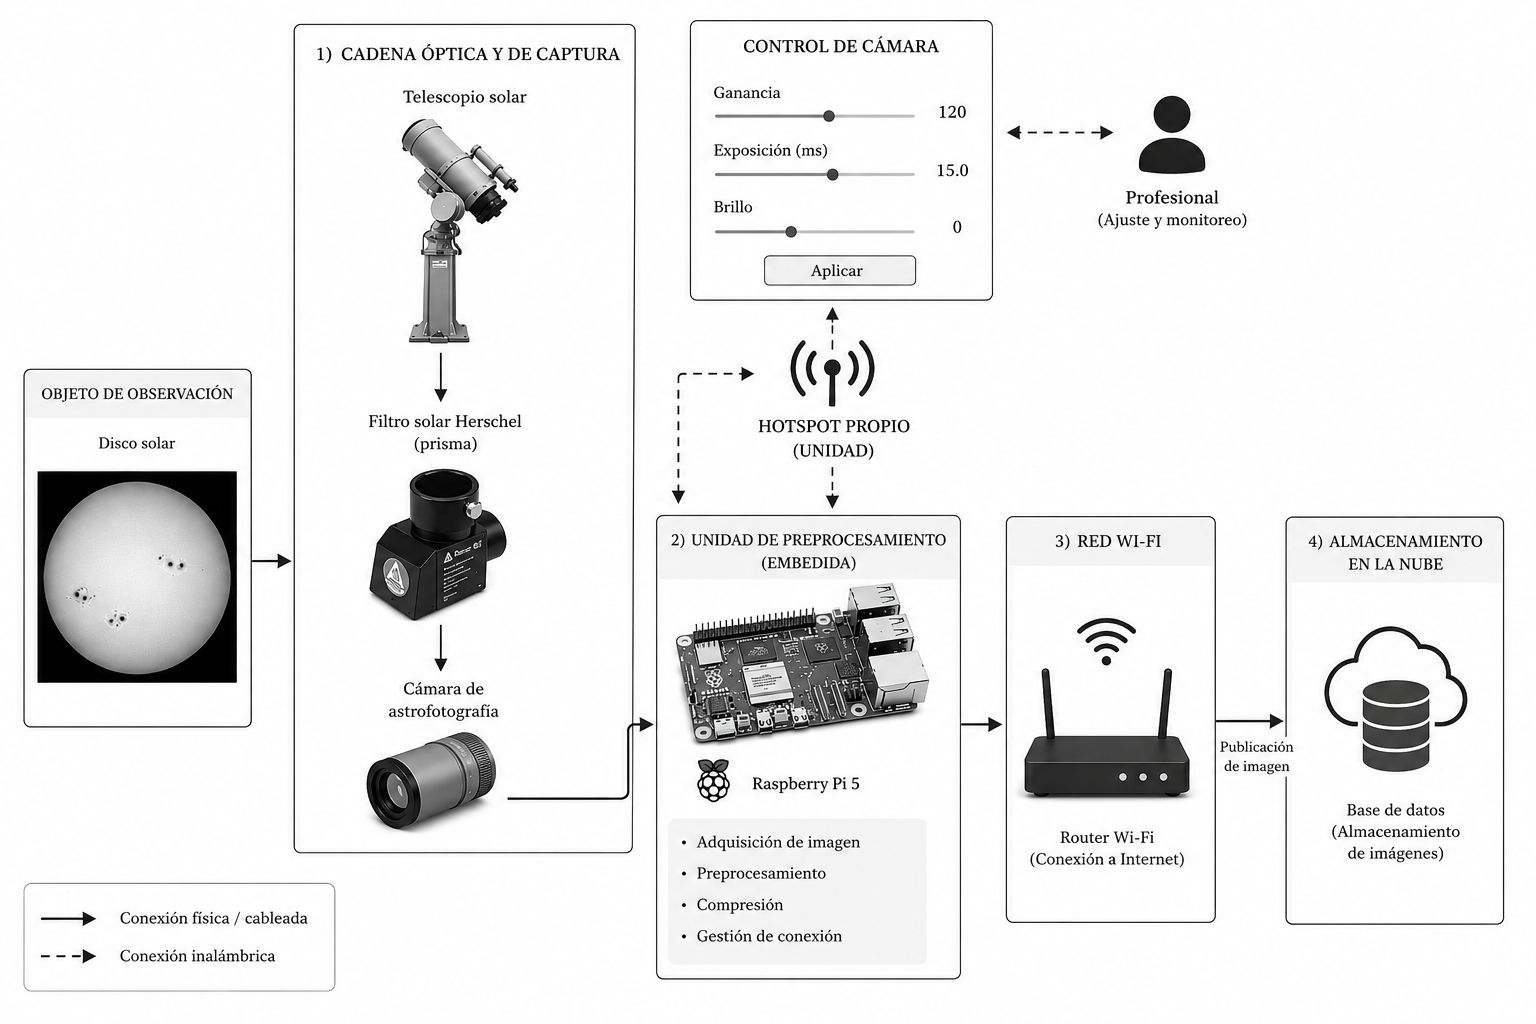
\includegraphics[height=0.7\textheight,width=\linewidth,keepaspectratio]{hw/module.png}
%         \small
%         Portabilidad, seguridad óptica, trazabilidad y despliegue local guían la selección.
%         \column{0.48\textwidth}
%         \scriptsize
%         \begin{table}
%             \centering
%             \setlength{\tabcolsep}{3pt}
%             \begin{tabular}{ll}
%                 \toprule
%                 \textbf{Componente} & \textbf{Justificación} \\
%                 \midrule
%                 Telescopio refractor & imagen solar estable \\
%                 Cuña de Herschel & atenuación segura \\
%                 Cámara monocromática & sensibilidad sin Bayer \\
%                 Raspberry Pi 5 & nodo de borde \\
%                 Pantalla local & diagnóstico autónomo \\
%                 \bottomrule
%             \end{tabular}
%         \end{table}
%     \end{columns}
% \end{frame}


\begin{frame}{Esquema Eléctrico del Módulo de Observación}
    \centering
    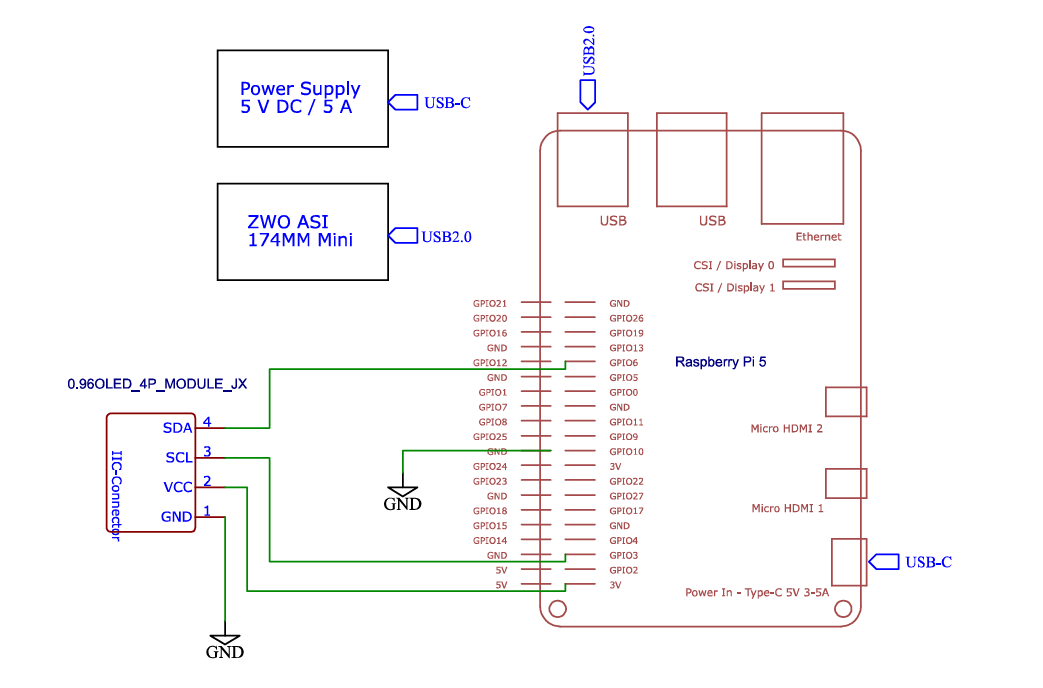
\includegraphics[height=0.76\textheight,width=0.96\linewidth,keepaspectratio]{hw/electric.png}
    \vspace{0.08cm}
\end{frame}

\begin{frame}{Costos del Prototipo}
    \centering
    \vfill

    \scriptsize \textbf{Presupuesto Referencial de Componentes del Prototipo}
    \vspace{0.1cm}

    % Configuración de tabla compacta y estética para Beamer sin la columna de cantidad
    \renewcommand{\arraystretch}{1.2}
    \setlength{\tabcolsep}{12pt} % Un poco más de separación al tener menos columnas
    \begin{table}
        \centering
        \scriptsize
        \begin{tabular}{lrr}
            \toprule
            \textbf{Componente} & \textbf{Precio (USD)} & \textbf{Precio (PYG)} \\
            \midrule
            Raspberry Pi 5 8 GB & 190 & 1.160.520 \\
            Módulo active cooler para Raspberry Pi 5 & 13 & 79.404 \\
            Cámara ZWO ASI174MM Mini & 432 & 2.638.656 \\
            Filtro solar Herschel wedge Lunt 1.25'' con ND3 & 308 & 1.881.264 \\
            Pantalla OLED 0.96'' 128x64 & 9 & 54.972 \\
            Impresión 3D de carcasa y soporte & 4 & 24.432 \\
            \midrule
            % Fila de TOTAL unificada y limpia con el fondo gris
            \rowcolor{black!12} \textbf{Total} & \textbf{956} & \textbf{5.839.248} \\
            \bottomrule
        \end{tabular}
    \end{table}

    \vspace{0.3cm}

    % Breve comentario cualitativo debajo de la tabla (1 USD = 6108 PYG)
    \begin{minipage}{0.85\linewidth}
        \centering
        \scriptsize\itshape
        La inversión total de hardware asciende a \textbf{5.839.248 PYG} (956 USD), consolidando una arquitectura basada en sistemas embebidos de bajo costo y alto rendimiento óptico para el procesamiento solar local.
    \end{minipage}

    \vfill
\end{frame}

\section{Diseño de Software}

\begin{frame}{Datos de Entrenamiento: HMI/SDO + SRS/NOAA}
    \begin{columns}
        \column{0.55\textwidth}
        \centering
        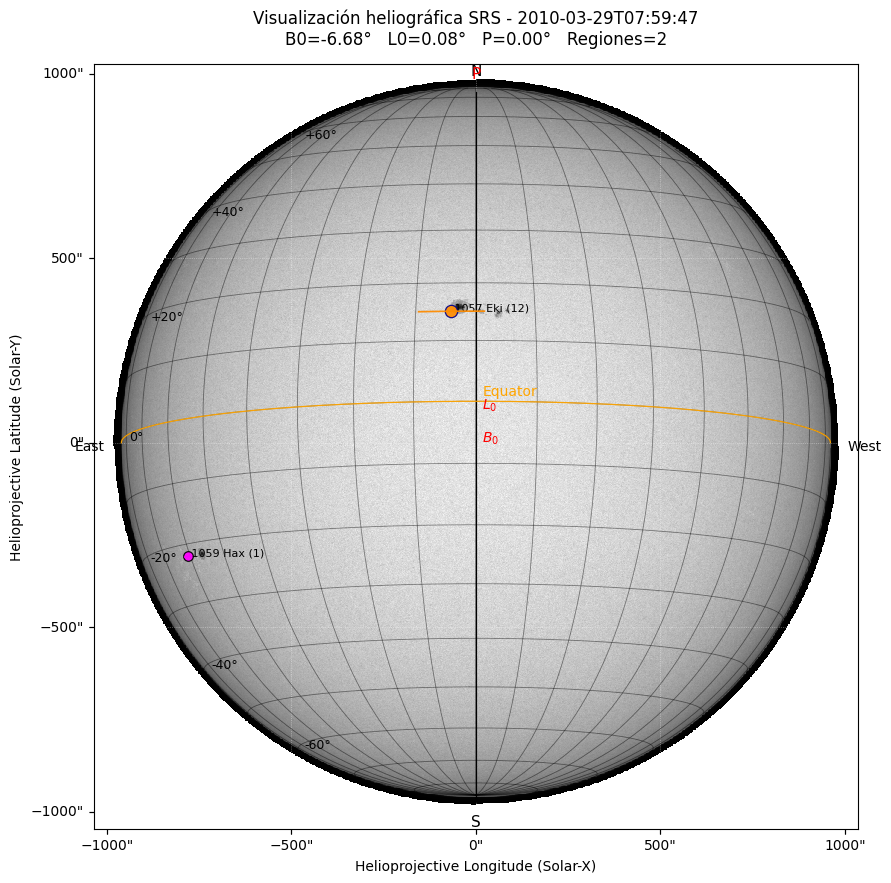
\includegraphics[height=0.55\textheight,width=\linewidth,keepaspectratio]{solar/helio_proj.png}\par
        \vspace{0.03cm}
        {\scriptsize Coordenadas solares a pixeles.}
        \column{0.49\textwidth}
        \centering
        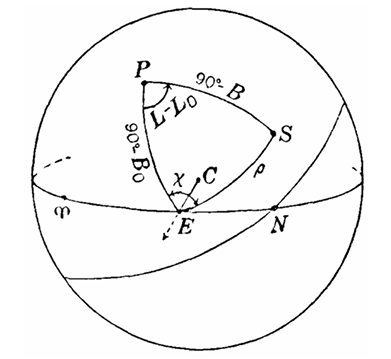
\includegraphics[height=0.52\textheight,width=\linewidth,keepaspectratio]{solar/helio_geom.png}\par
        \vspace{0.03cm}
        {\scriptsize Proyección heliográfica de detecciones [12].}
    \end{columns}
    
    \vfill
    {\tiny\color{gray} [12] ESA CESAR Education Team, “Heliographic Coordinates Project Booklet,” ESA Publications, 2024.}
\end{frame}

\begin{frame}{Datos de Entrenamiento: Discretización de Base de Datos}
    \centering
    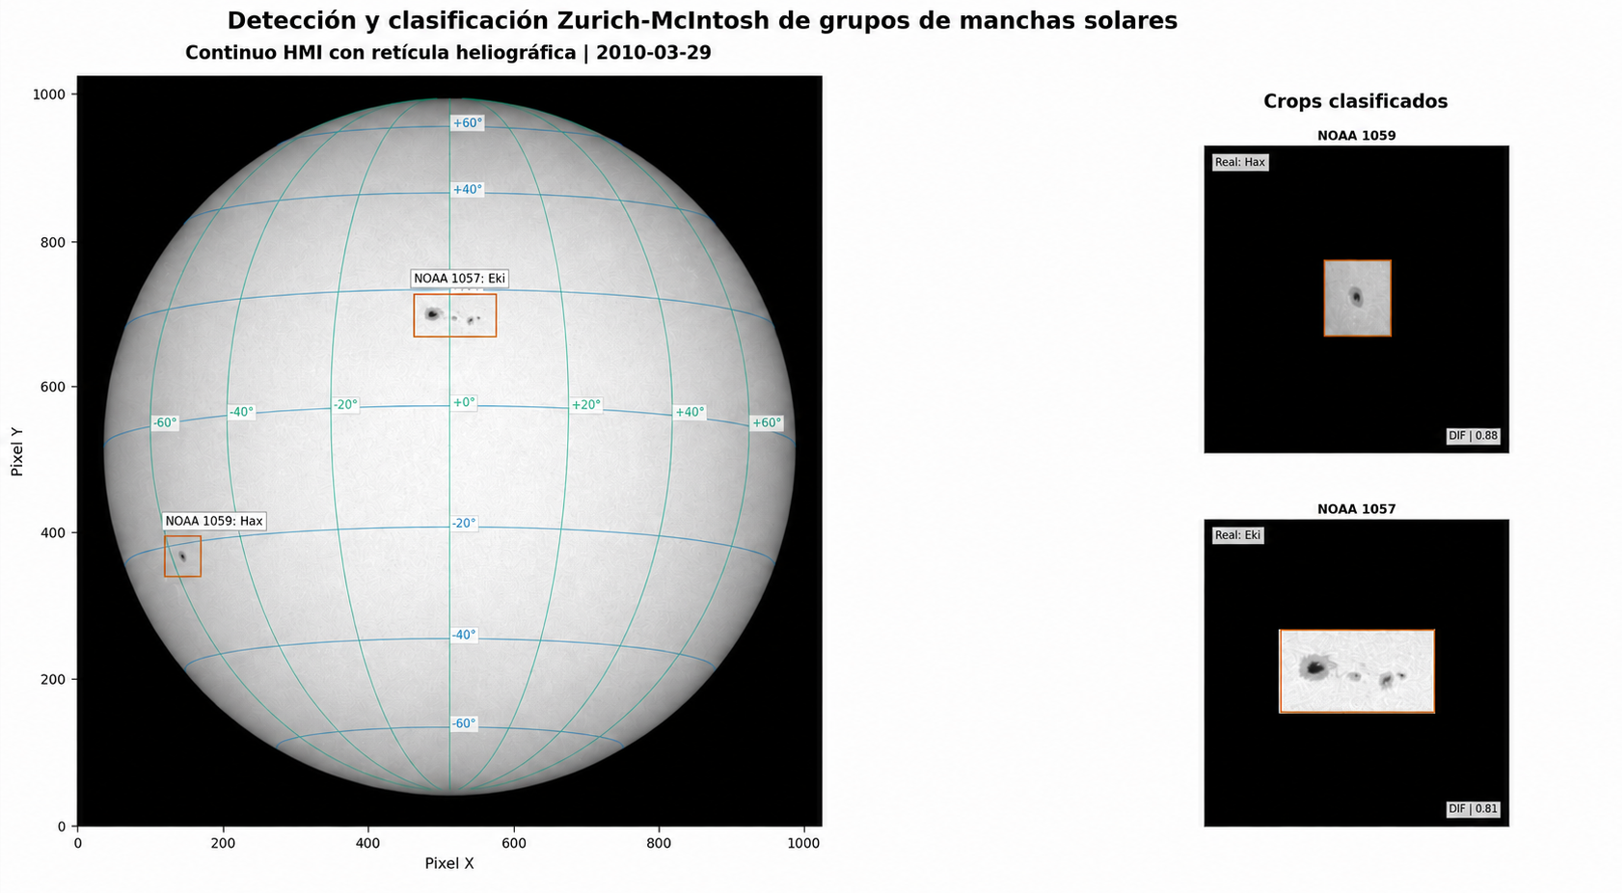
\includegraphics[height=0.9\textheight,width=0.92\linewidth,keepaspectratio]{data/db2_build.png}
    \vspace{0.08cm}
\end{frame}

\begin{frame}{Datos de Entrenamiento: Datasets generados (2010--2025)}
    \vspace{-0.4cm} % Sube el recuadro para que quede alineado con el título
    
    % Envuelve el cuadro y lo empuja hacia el extremo derecho exacto
    \begin{columns}[t]
        \begin{column}{\textwidth}
            \hfill
            \setlength{\fboxrule}{1.2pt} % Grosor del borde
            \setlength{\fboxsep}{4pt}    % Margen interno del cuadro
            \fcolorbox{llamativoMagenta}{white}{%
                \scriptsize\textcolor{llamativoMagenta}{\textbf{Contribución 2}}
            }
        \end{column}
    \end{columns}
    \footnotesize
    \begin{block}{DB1 -- detección de grupos solares (Para YOLO26n)}
      \begin{itemize}
            \item \textbf{4700 im\'agenes} de disco solar completo en \textbf{1024\,$\times$\,1024 px}.
            \item Incluye \textit{bounding boxes} de agrupamiento solar para entrenamiento tipo YOLO.
      \end{itemize}
    \end{block}

    \begin{block}{DB2 -- clasificación morfológica (Etapa preeliminar)}
        \begin{itemize}
            \item \textbf{15000 recortes} derivados de los \textit{bounding boxes} de DB1 de \textbf{224\,$\times$\,224 px}
            \item Incluye etiquetas $ZPC$ de SRS/NOAA [12].
        \end{itemize}
    \end{block}

    \begin{block}{DB2.1 -- clasificación morfológica refinada (Para ConvNeXtV2a)}
        \begin{itemize}
            \item \textbf{14700 recortes} derivados de DB2 de \textbf{224\,$\times$\,224 px} refinado con \textbf{PCA} de 60 componentes principales.
            \item Incluye etiquetas $ZPC$ de SRS/NOAA [12].
        \end{itemize}
    \end{block}
    
    \vfill
    {\tiny\color{gray} [12] NOAA Space Weather Prediction Center, “Solar Region Summary (SRS) Data Logs,” 2025.}
\end{frame}

\begin{frame}{Datos de Entrenamiento: Conflicto de operatividad}
    
    \vspace{0.2cm} % Margen inicial sutil debajo del título del frame

    % [c] fuerza a que TODOS los elementos de las columnas se alineen horizontalmente por su centro geométrico
    \begin{columns}[c]
        
        % Columna 1: SIDC / USET
        \begin{column}{0.31\textwidth}
            \centering
            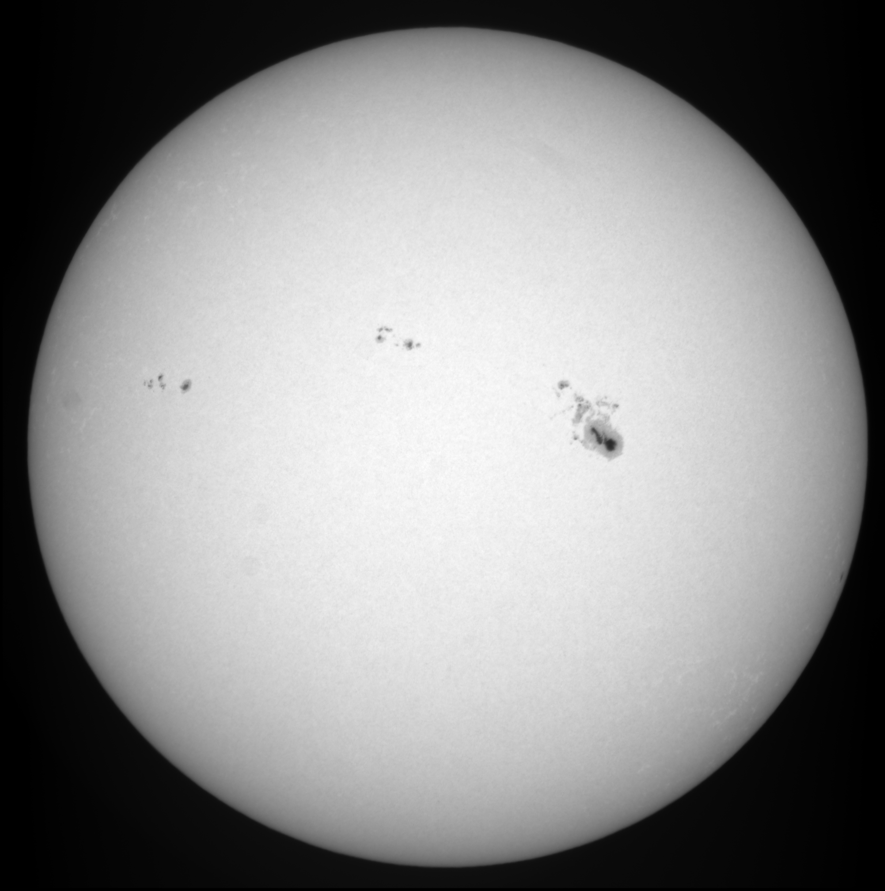
\includegraphics[height=0.5\textheight, width=\linewidth, keepaspectratio]{data/wl.png}\par
            \vspace{0.08cm}
            {\tiny Luz Blanca\\(Terrestre SIDC/USET)}
        \end{column}
        
        % Columna 2: SDO / NASA
        \begin{column}{0.31\textwidth}
            \centering
            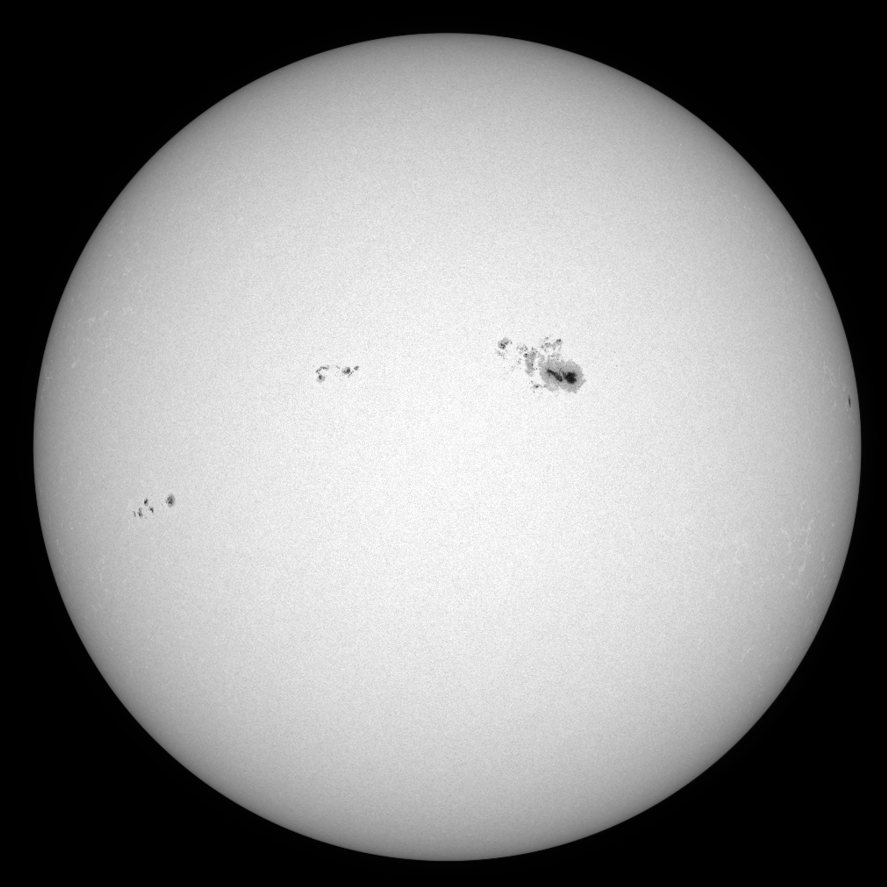
\includegraphics[height=0.5\textheight, width=\linewidth, keepaspectratio]{data/hmi.png}\par
            \vspace{0.08cm}
            {\tiny Imagen HMI\\(Satélite SDO/NASA)}
        \end{column}
        
        % Columna 3: Nota técnica en cuadro de bordes curvos y fondo magenta
        \begin{column}{0.34\textwidth}
            % Configuración local de colores para la caja curva
            \setbeamercolor{cajaMagenta}{fg=white, bg=llamativoMagenta}
            
            \begin{beamercolorbox}[wd=\linewidth, rounded=true, sep=6pt]{cajaMagenta}
                \scriptsize
                \textbf{Efecto de Paralaje}
                \vspace{0.1cm}
                
                El emparejamiento SDO-SIDC introduce un paralaje geométrico debido a la diferencia de perspectiva espacial-terrestre.
                \vspace{0.12cm}
                
                Sin embargo, al no haber cambios morfológicos significativos, este efecto se considera \textbf{despreciable} para la clasificación.
            \end{beamercolorbox}
        \end{column}
        
    \end{columns}

    \vfill % Empuja de forma exacta y limpia las referencias al límite inferior de la diapositiva

    % Referencias en la base de la pantalla (Espacio totalmente garantizado)
    % {\tiny\color{gray}
    % [11] Pesnell, W. D., et al. (2012). The Solar Dynamics Observatory. \textit{Solar Physics.}
    % }
    
    % {\tiny\color{gray}
    % [12] Clette, F., et al. (2014). Revisiting the Sunspot Number. \textit{Space Science Reviews.}
    % }
\end{frame}

\begin{frame}{Modelos predictivos: Modelo escalar de Podladchikova con filtro Kalman (PVLK)}
    \centering
    \small
    
    \vspace{0.1cm}
    \begin{columns}[T]
        % Columna Izquierda: Ecuaciones y flujo del filtro
        \begin{column}{0.65\textwidth}
            \footnotesize
            \textbf{1. Modelo Paramétrico PVL (Forma del ciclo):}
            \begin{equation*}
                f(v; a, b) = \frac{a \cdot v^3}{\exp(v^2/b^2) - 0.71} \quad \text{con } b=27.12 + 25.15(1000a)^{-1/4}
            \end{equation*}

            \textbf{2. Ruido Adaptativo e Inyección de $Q_k$:}
            \begin{equation*}
                Q_k = 0.2 \Phi_k \hat{s}_{k-1}, \quad R_k = 2.5 \Phi_k \hat{s}_{k-1} \quad \rightarrow \quad P_k^- = \Phi_k^2 P_{k-1} + Q_k
            \end{equation*}

            \textbf{3. Ganancia de Kalman ($K_k$) y Actualización:}
            \begin{equation*}
                K_k = \frac{P_k^-}{P_k^- + R_k} \quad \rightarrow \quad \hat{s}_k = \Phi_k \hat{s}_{k-1} + K_k (z_k - \Phi_k \hat{s}_{k-1})
            \end{equation*}
        \end{column}
        
        % Columna Derecha: Tabla de variables optimizada
        \begin{column}{0.32\textwidth}
            \vspace{0.3cm}
            \centering
            \footnotesize
            \renewcommand{\arraystretch}{1.2}
            \begin{tabular}{c|l}
                \textbf{Var.} & \textbf{Descripción} \\ \hline
                $v$ & Tiempo (meses) \\
                $a, b$ & Parámetros PVL \\
                $\Phi_k$ & Transición: $\frac{f(v_k)}{f(v_{k-1})}$ \\
                $\hat{s}_k$ & Estado ($SSN_{\mathrm{PVLK}}$) \\
                $P_k$ & Varianza del error \\
                $z_k$ & Medición real (SSN) \\
            \end{tabular}
        \end{column}
    \end{columns}

    \vspace{0.3cm}
    
    {\footnotesize El escalado dinámico de $Q_k$ y $R_k$ recalcula continuamente la ganancia $K_k$, mitigando la heterocedasticidad de la serie temporal [11].}

    \vfill
    {\tiny\color{gray} [11] Podladchikova, T. y Van der Linden, R. (2011). Kalman Filter Technique for Improving Prediction of Smoothed Monthly Sunspot Numbers. Solar Physics, 271(2), 469–485.\par}
\end{frame}

\begin{frame}{Modelos predictivos: Vectorización del diagrama de Spörer}
    \vspace{-0.7cm} % Sube el recuadro para que quede alineado con el título
    
    % Envuelve el cuadro y lo empuja hacia el extremo derecho exacto
    \begin{columns}[t]
        \begin{column}{\textwidth}
            \hfill
            \setlength{\fboxrule}{1.2pt} % Grosor del borde
            \setlength{\fboxsep}{4pt}    % Margen interno del cuadro
            \fcolorbox{llamativoMagenta}{white}{%
                \scriptsize\textcolor{llamativoMagenta}{\textbf{Contribución 3}}
            }
        \end{column}
    \end{columns}

    \centering
    \begin{center}
        \makebox[\linewidth][c]{%
            % Ajusta el 1.5 a 1.8, 2.0, etc., según qué tan aumentada la necesites
            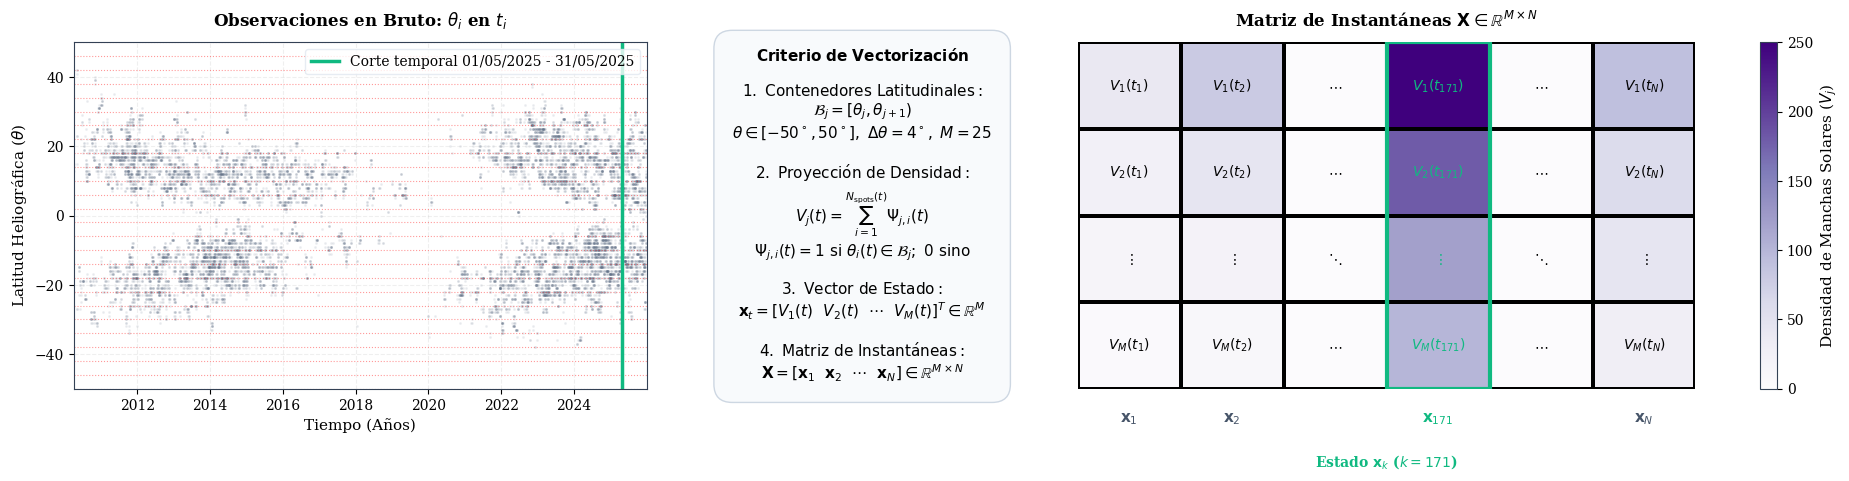
\includegraphics[width=1.0\paperwidth, keepaspectratio]{dmd/discretizacion.png}%
        }
    \end{center}
\end{frame}


\begin{frame}{Modelos predictivos: Modelo vectorial con Dynamic Mode Decomposition (DMD)}
    \centering
    \vfill
    \begin{minipage}{0.75\linewidth}
        \begin{center}
        \makebox[\linewidth][c]{%
            % Ajusta el 1.5 a 1.8, 2.0, etc., según qué tan aumentada la necesites
            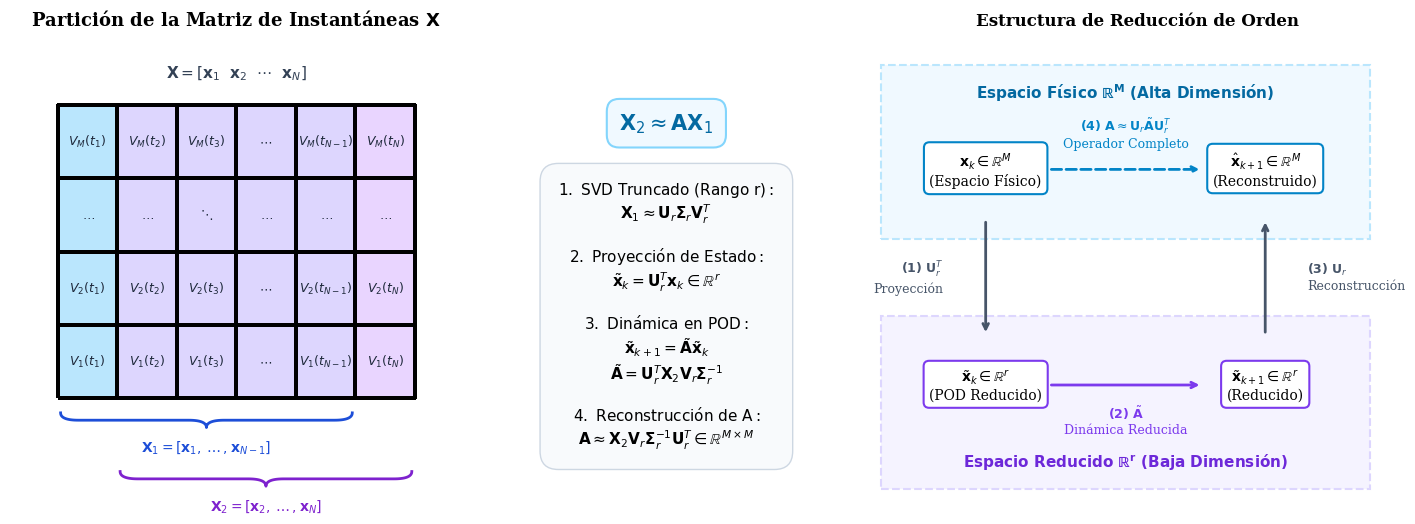
\includegraphics[width=0.98\paperwidth, keepaspectratio]{dmd/dmd.png}%
        }
        \end{center}
    \end{minipage}\par
    
    \vfill
    {\tiny\color{gray} [12] Brunton, S. L., & Kutz, J. N. (2016). Dynamic Mode Decomposition: Data-Driven Modeling of Complex Systems. Society for Industrial and Applied Mathematics (SIAM).\par}
\end{frame}

\begin{frame}{Modelos predictivos: Modelo vectorial DMD VS Modelo escalar PVL+Kalman}
    \centering
    \vfill
    \begin{minipage}{0.9\linewidth}
        \begin{center}
        \makebox[\linewidth][c]{%
            % Ajusta el 1.5 a 1.8, 2.0, etc., según qué tan aumentada la necesites
            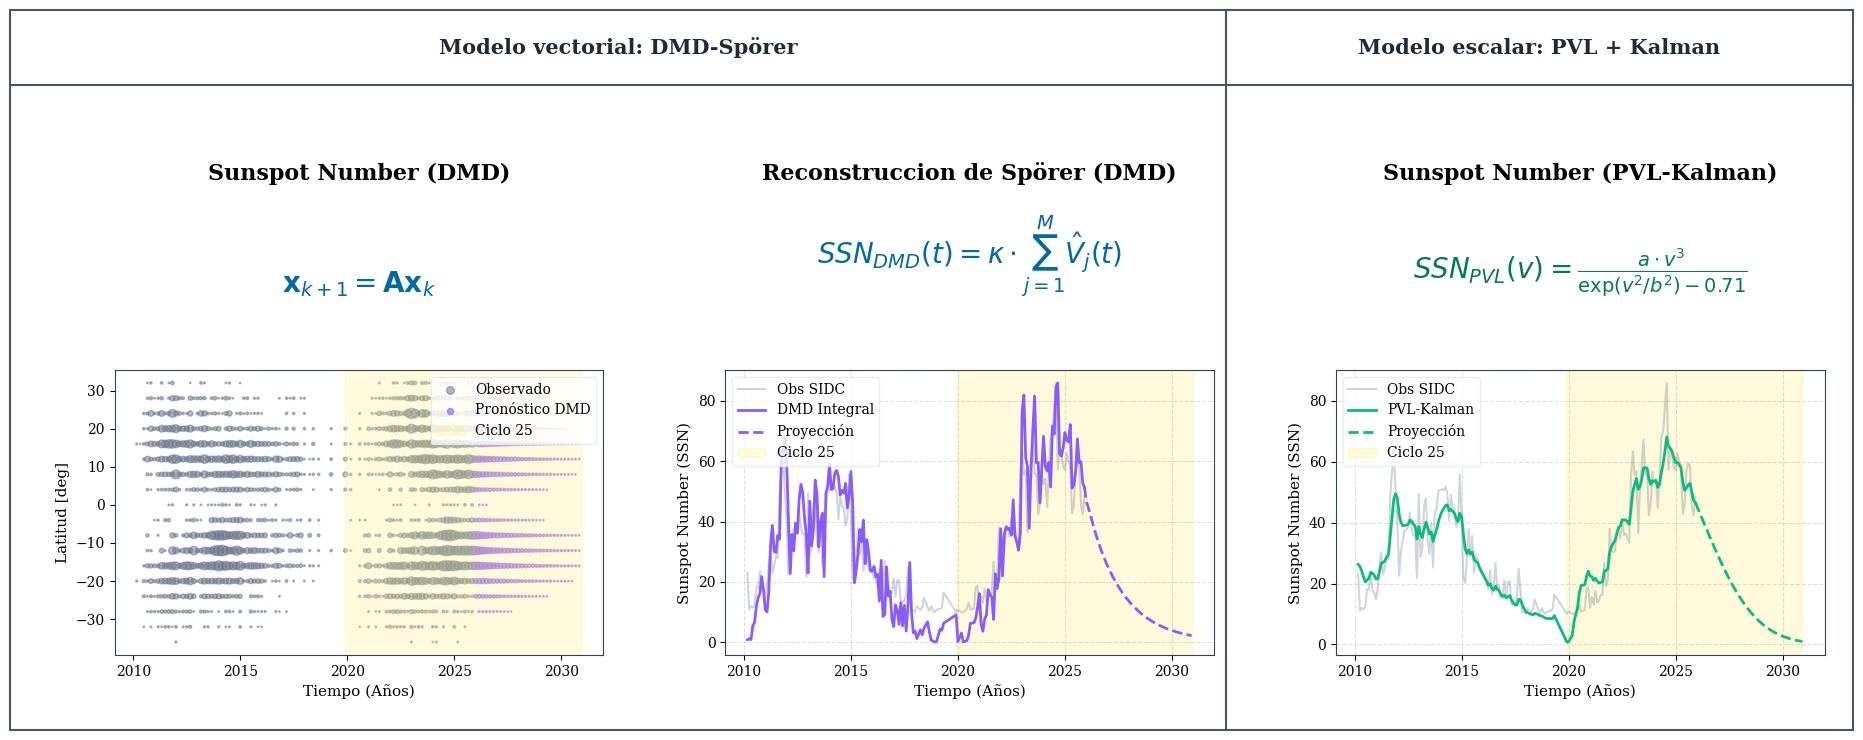
\includegraphics[width=0.95\paperwidth, keepaspectratio]{dmd/model_results.png}%
        }
        \end{center}
    \end{minipage}\par
\end{frame}

\begin{frame}{Modelos de Deep Learning en Cascada}
    \vspace{-0.4cm} % Sube el recuadro para que quede alineado con el título
    
    % Envuelve el cuadro y lo empuja hacia el extremo derecho exacto
    \begin{columns}[t]
        \begin{column}{\textwidth}
            \hfill
            \setlength{\fboxrule}{1.2pt} % Grosor del borde
            \setlength{\fboxsep}{4pt}    % Margen interno del cuadro
            \fcolorbox{llamativoMagenta}{white}{%
                \scriptsize\textcolor{llamativoMagenta}{\textbf{Contribución 4}}
            }
        \end{column}
    \end{columns}
    \centering
    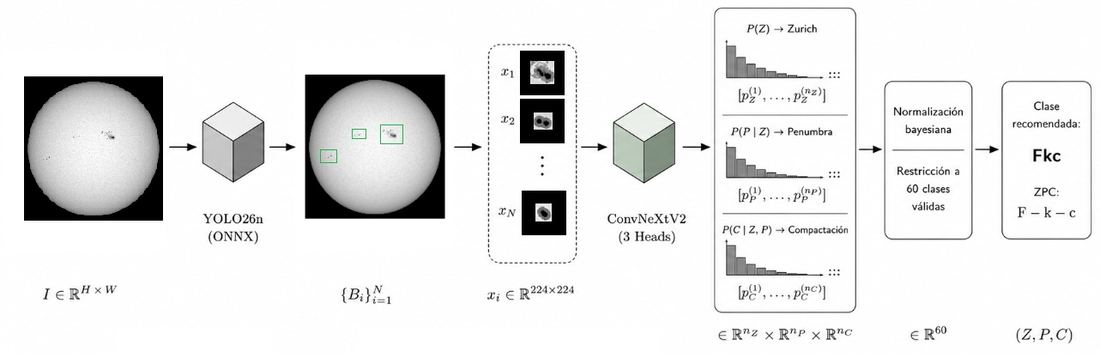
\includegraphics[height=0.92\textheight,width=0.96\linewidth,keepaspectratio]{sys/img_pipe.jpg}
    \vspace{0.08cm}
\end{frame}

\begin{frame}[fragile]{Modelos de Deep Learning en Cascada: Entrenamiento de Yolo26n}
    \small
    \begin{columns}[T]
        \begin{column}{0.58\linewidth}
    {\scriptsize
    \begin{lstlisting}[language=Python]
    model.train(
        data="/data.yaml",
        epochs=200, 
        imgsz=640,
        batch=8,
        optimizer="SGD",
        workers=0, cache=False,
        **best_hps
    )
    \end{lstlisting}
    }
            \end{column}
            \begin{column}{0.38\linewidth}
                \begin{itemize}
                    \item Se emplea \texttt{best\_hps = study.best\_params} tras búsqueda previa con Optuna [20].
                    \item El entrenamiento se ejecuta por 200 \textit{epochs}.
                    \item La configuración prioriza equilibrio entre precisión y factibilidad embebida.
                \end{itemize}
            \end{column}
        \end{columns}
        
        \vfill
        {\tiny\color{gray} [13] T. Akiba et al., “Optuna: A next-generation hyperparameter optimization framework,” in Proc. ACM SIGKDD, 2019.}
    \end{frame}

\begin{frame}{Modelos de Deep Learning en Cascada: Entrenamiento de Yolo26n}
    \centering
    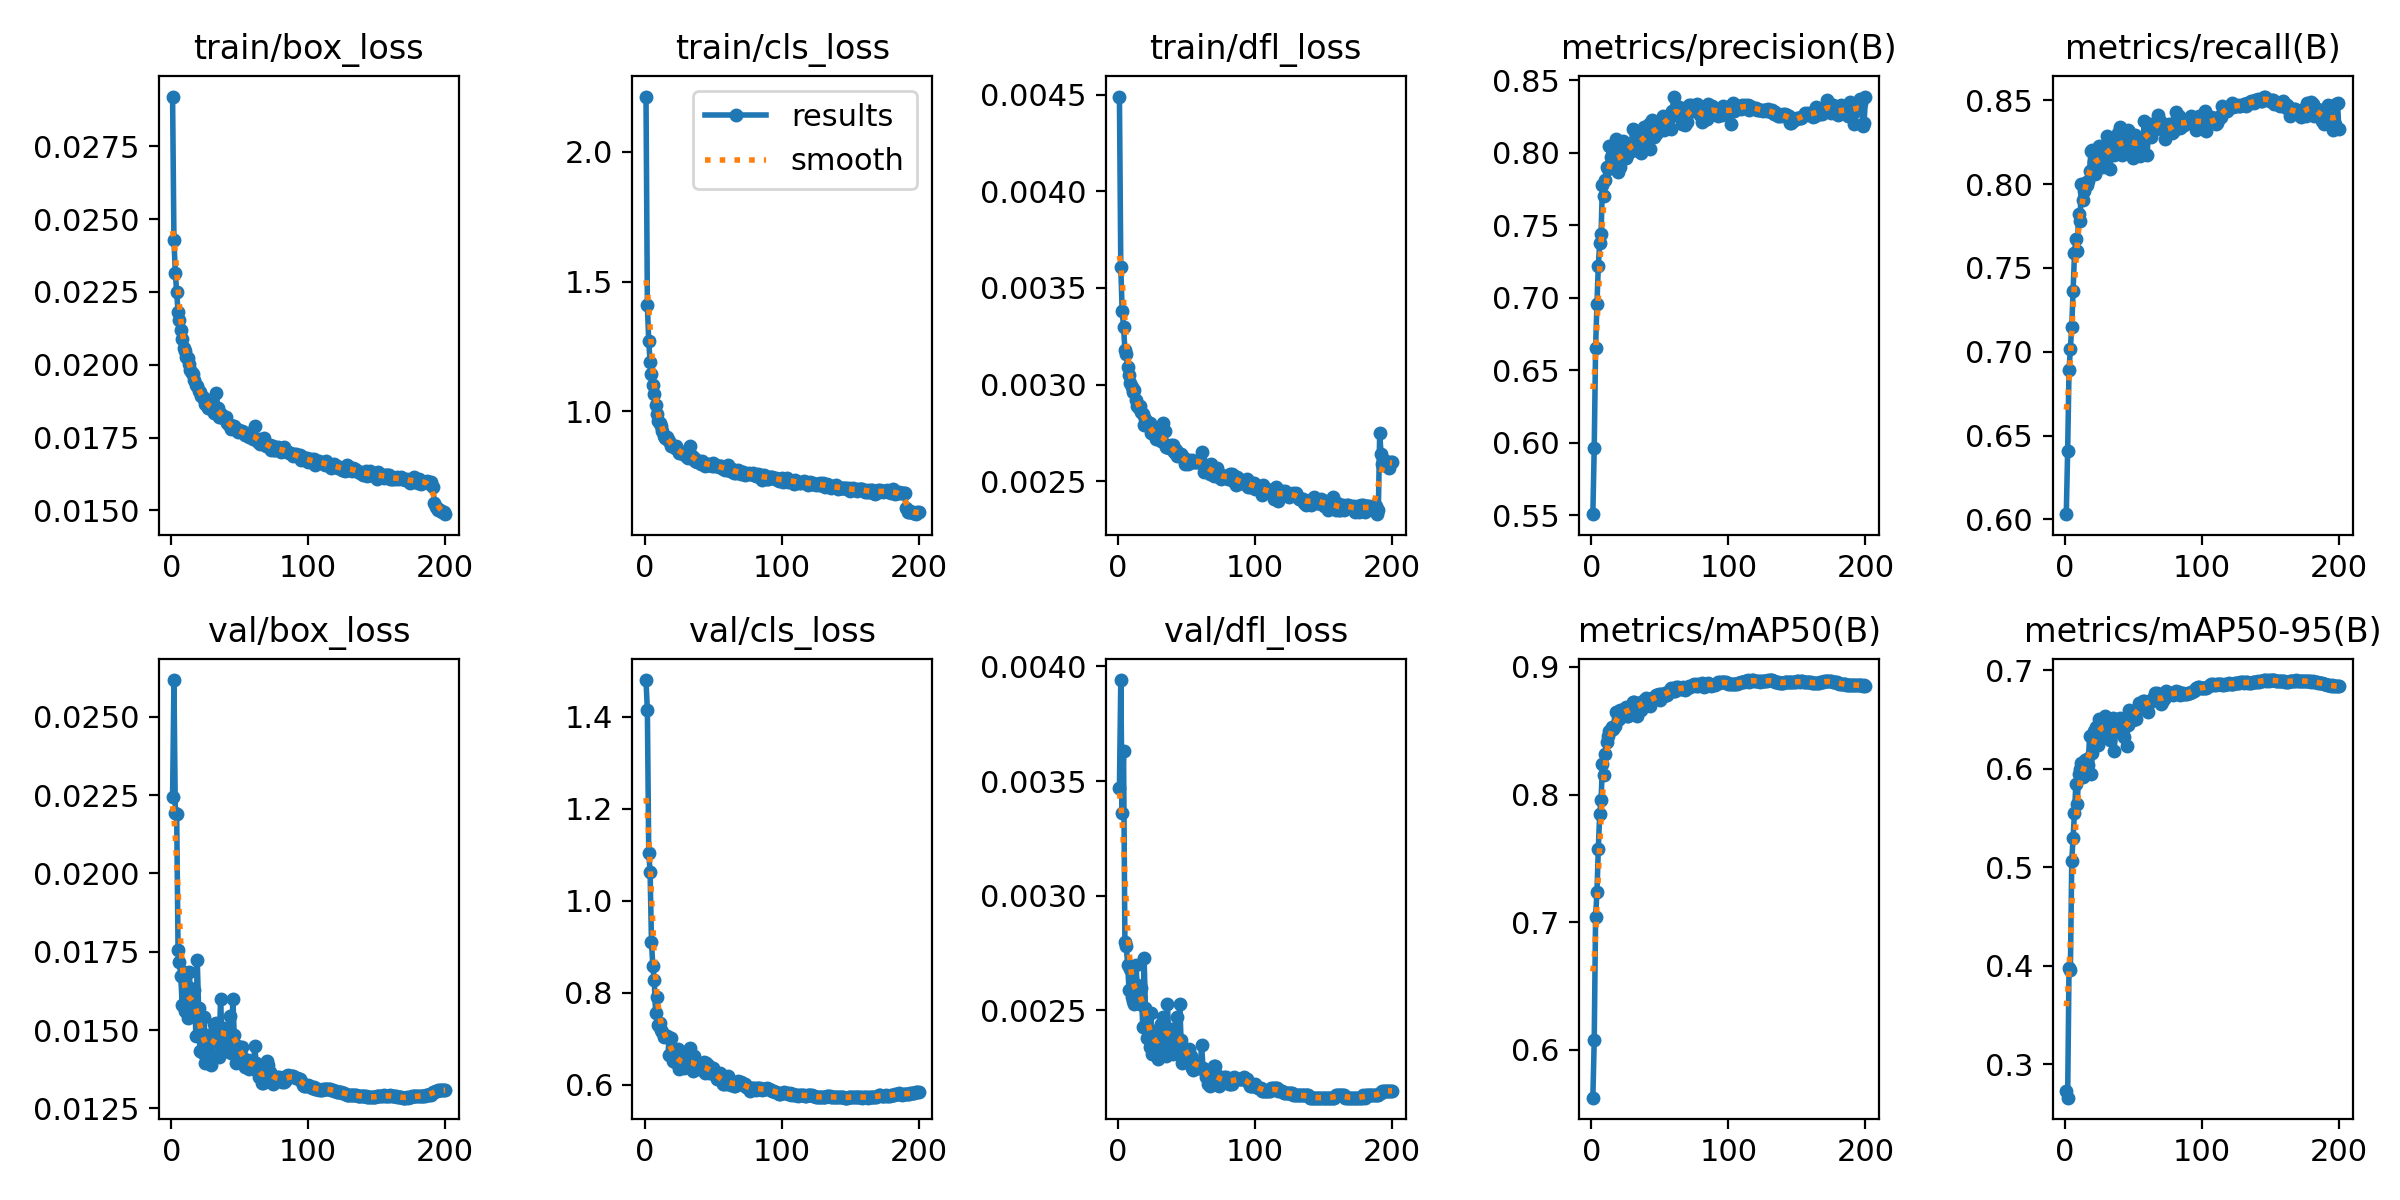
\includegraphics[height=0.92\textheight,width=0.96\linewidth,keepaspectratio]{ml/yolo_results.png}
    \vspace{0.08cm}
\end{frame}

\begin{frame}{Modelos de Deep Learning en Cascada: Entrenamiento de Arquitectura jerárquica ConvNeXtv2a}
    \centering
    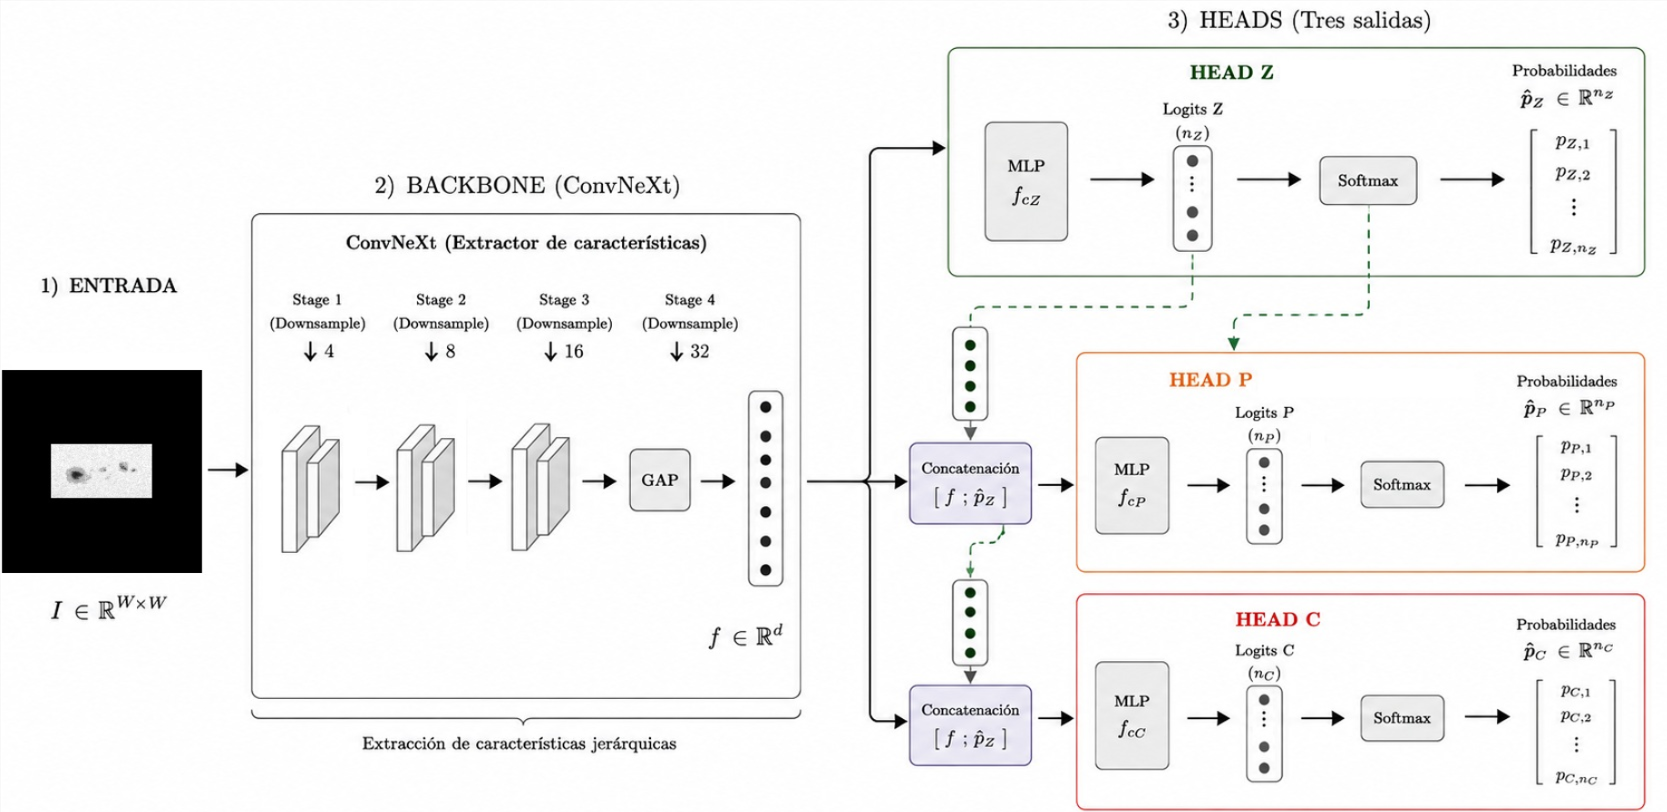
\includegraphics[height=0.75\textheight,width=0.96\linewidth,keepaspectratio]{ml/convnext_arch.png}
    \vspace{0.08cm}
\end{frame}

\begin{frame}{Modelos de Deep Learning en Cascada: Entrenamiento de Arquitectura jerárquica ConvNeXtv2a}
    \small
    \begin{itemize}
        \item Para mitigar el desbalance de clases se utilizaron \textbf{Class-Balanced Weights} basados en el \textit{Effective Number of Samples} [14].
        \item Adem\'as, se incorpor\'o \textbf{remuestreo ponderado} mediante \textbf{\texttt{WeightedRandomSampler}}, reforzando la exposici\'on de clases minoritarias durante el entrenamiento.
    \end{itemize}
    
    \vfill
    {\tiny\color{gray} [14] Y. Cui et al., “Class-balanced loss based on effective number of samples,” in Proc. IEEE/CVF CVPR, 2019, pp. 9268--9277.}
\end{frame}

\begin{frame}{Modelos de Deep Learning en Cascada: Entrenamiento de Arquitectura jerárquica ConvNeXtv2a}
    \centering
    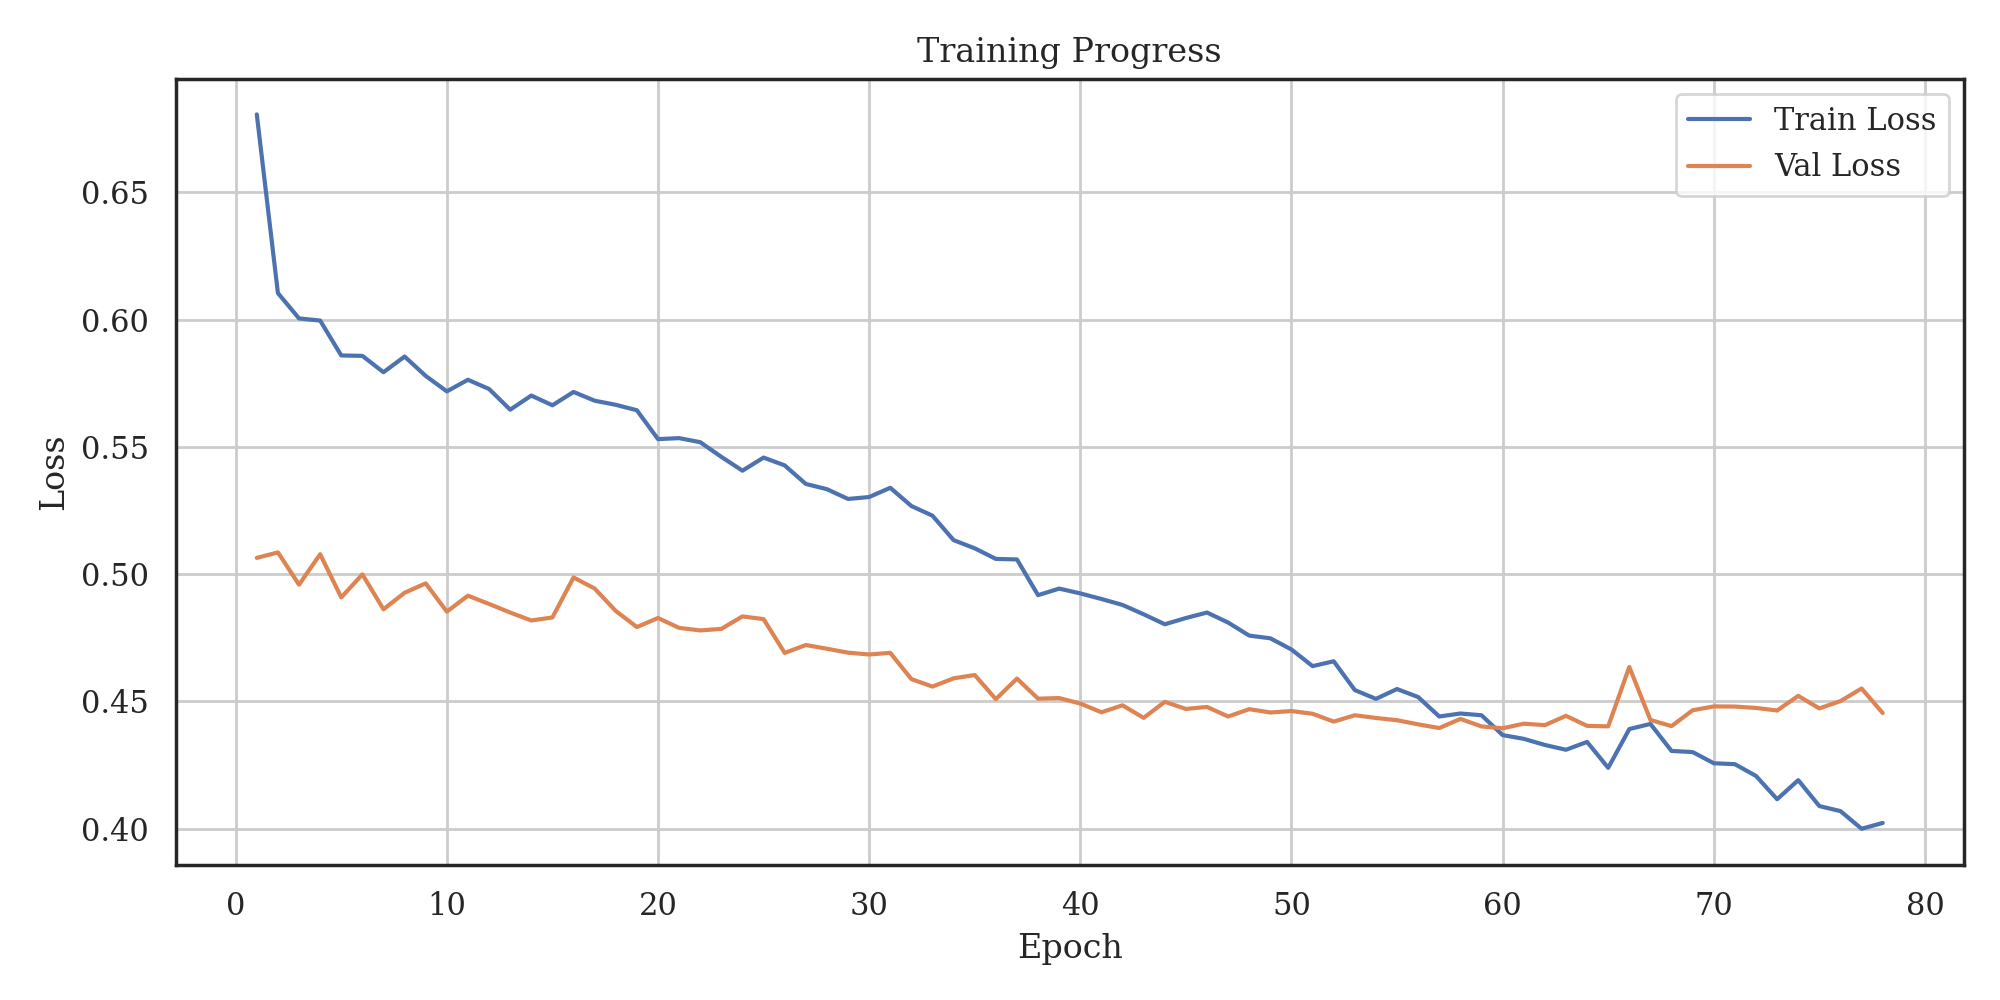
\includegraphics[height=0.78\textheight,width=0.96\linewidth,keepaspectratio]{ml/training_progress_classifier.png}
    \vspace{0.08cm}
\end{frame}

\begin{frame}{Modelos de Deep Learning en Cascada: Entrenamiento de Arquitectura jerárquica ConvNeXtv2a}
    \centering
    \begin{columns}[T]
        \begin{column}{0.4\linewidth}
            \centering
            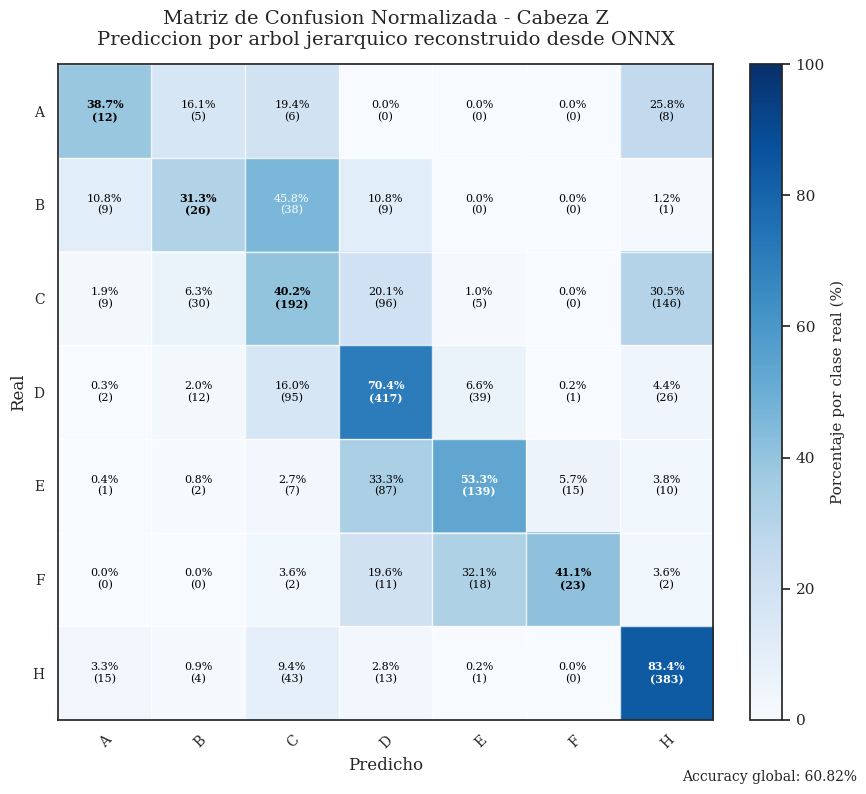
\includegraphics[width=\linewidth]{ml/conf_z.png}\par
            {\tiny Matriz de confusión para Z.}
        \end{column}
        \begin{column}{0.4\linewidth}
            \centering
            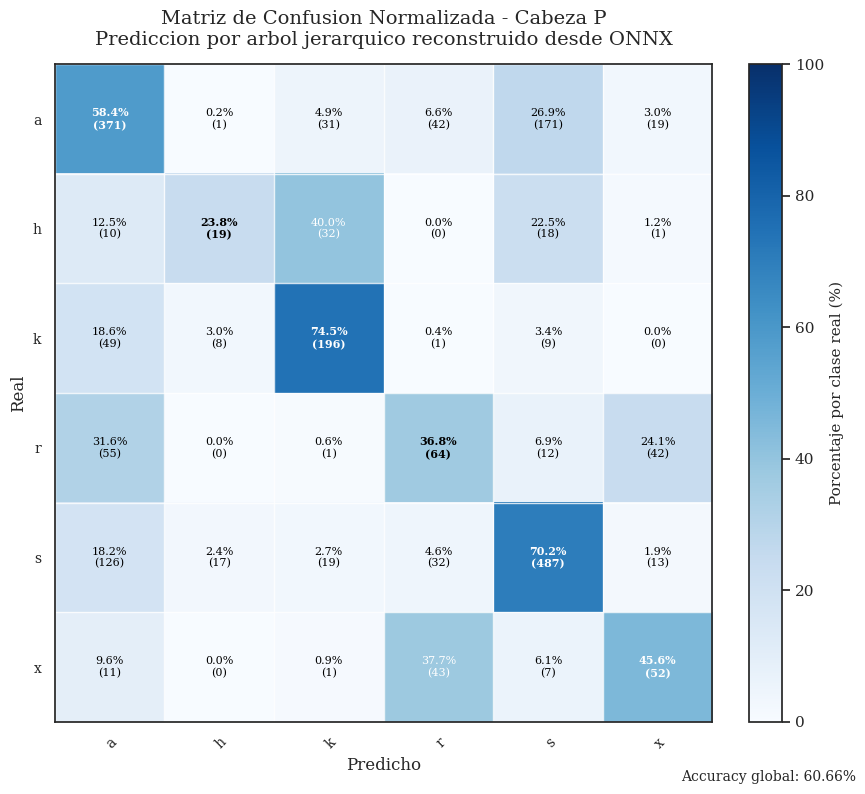
\includegraphics[width=\linewidth]{ml/conf_p.png}\par
            {\tiny Matriz de confusión para P.}
        \end{column}
        \begin{column}{0.4\linewidth}
            \centering
            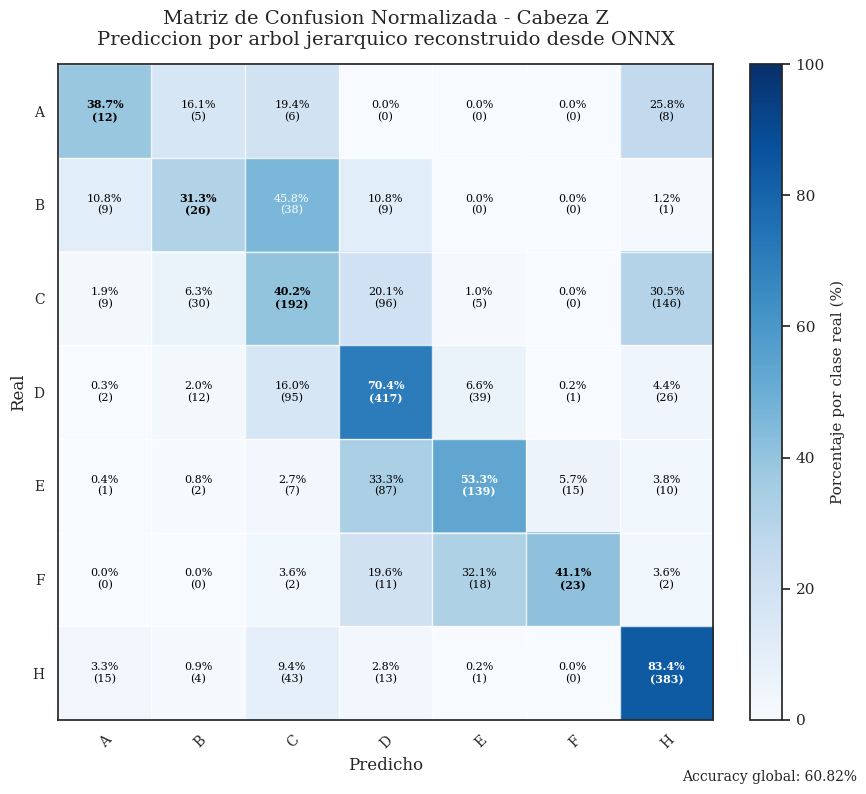
\includegraphics[width=\linewidth]{ml/conf_c.png}\par
            {\tiny Matriz de confusión para C.}
        \end{column}
    \end{columns}
\end{frame}

\begin{frame}{Modelos de Deep Learning en Cascada: Formalismo de la normalización Bayesiana}
    \centering
    \small
    \begin{align*}
        P(Z,P,C\mid x)&=P(Z\mid x)P(P\mid Z,x)P(C\mid Z,P,x),\\
        P_{\mathrm{base}}(Z,P,C\mid x)&=P(Z\mid x)P(P\mid x)P(C\mid x),\\
        P_{\mathrm{rec}}(Z,P,C\mid x)&=
        \frac{P_{\mathrm{base}}(Z,P,C\mid x)M_{ZPC}}
        {\sum_{z,p,c}P_{\mathrm{base}}(z,p,c\mid x)M_{zpc}}.
    \end{align*}
    \begin{equation*}
        (Z^\ast,P^\ast,C^\ast)=\arg\max_{Z,P,C}P_{\mathrm{rec}}(Z,P,C\mid x).
    \end{equation*}\par
    \vspace{0.05cm}
    {\footnotesize La máscara $M_{ZPC}$ anula combinaciones no admisibles de la taxonomía, es decir $\{ \# Z \} \cdot \{ \# P \} \cdot \{ \# C \} = 7 \times 6 \times 4 = 168$ a las $60$ clases validas.}
\end{frame}

\begin{frame}{Modelos de Deep Learning en Cascada: Árbol de recomendaciones semánticas}
    \centering
    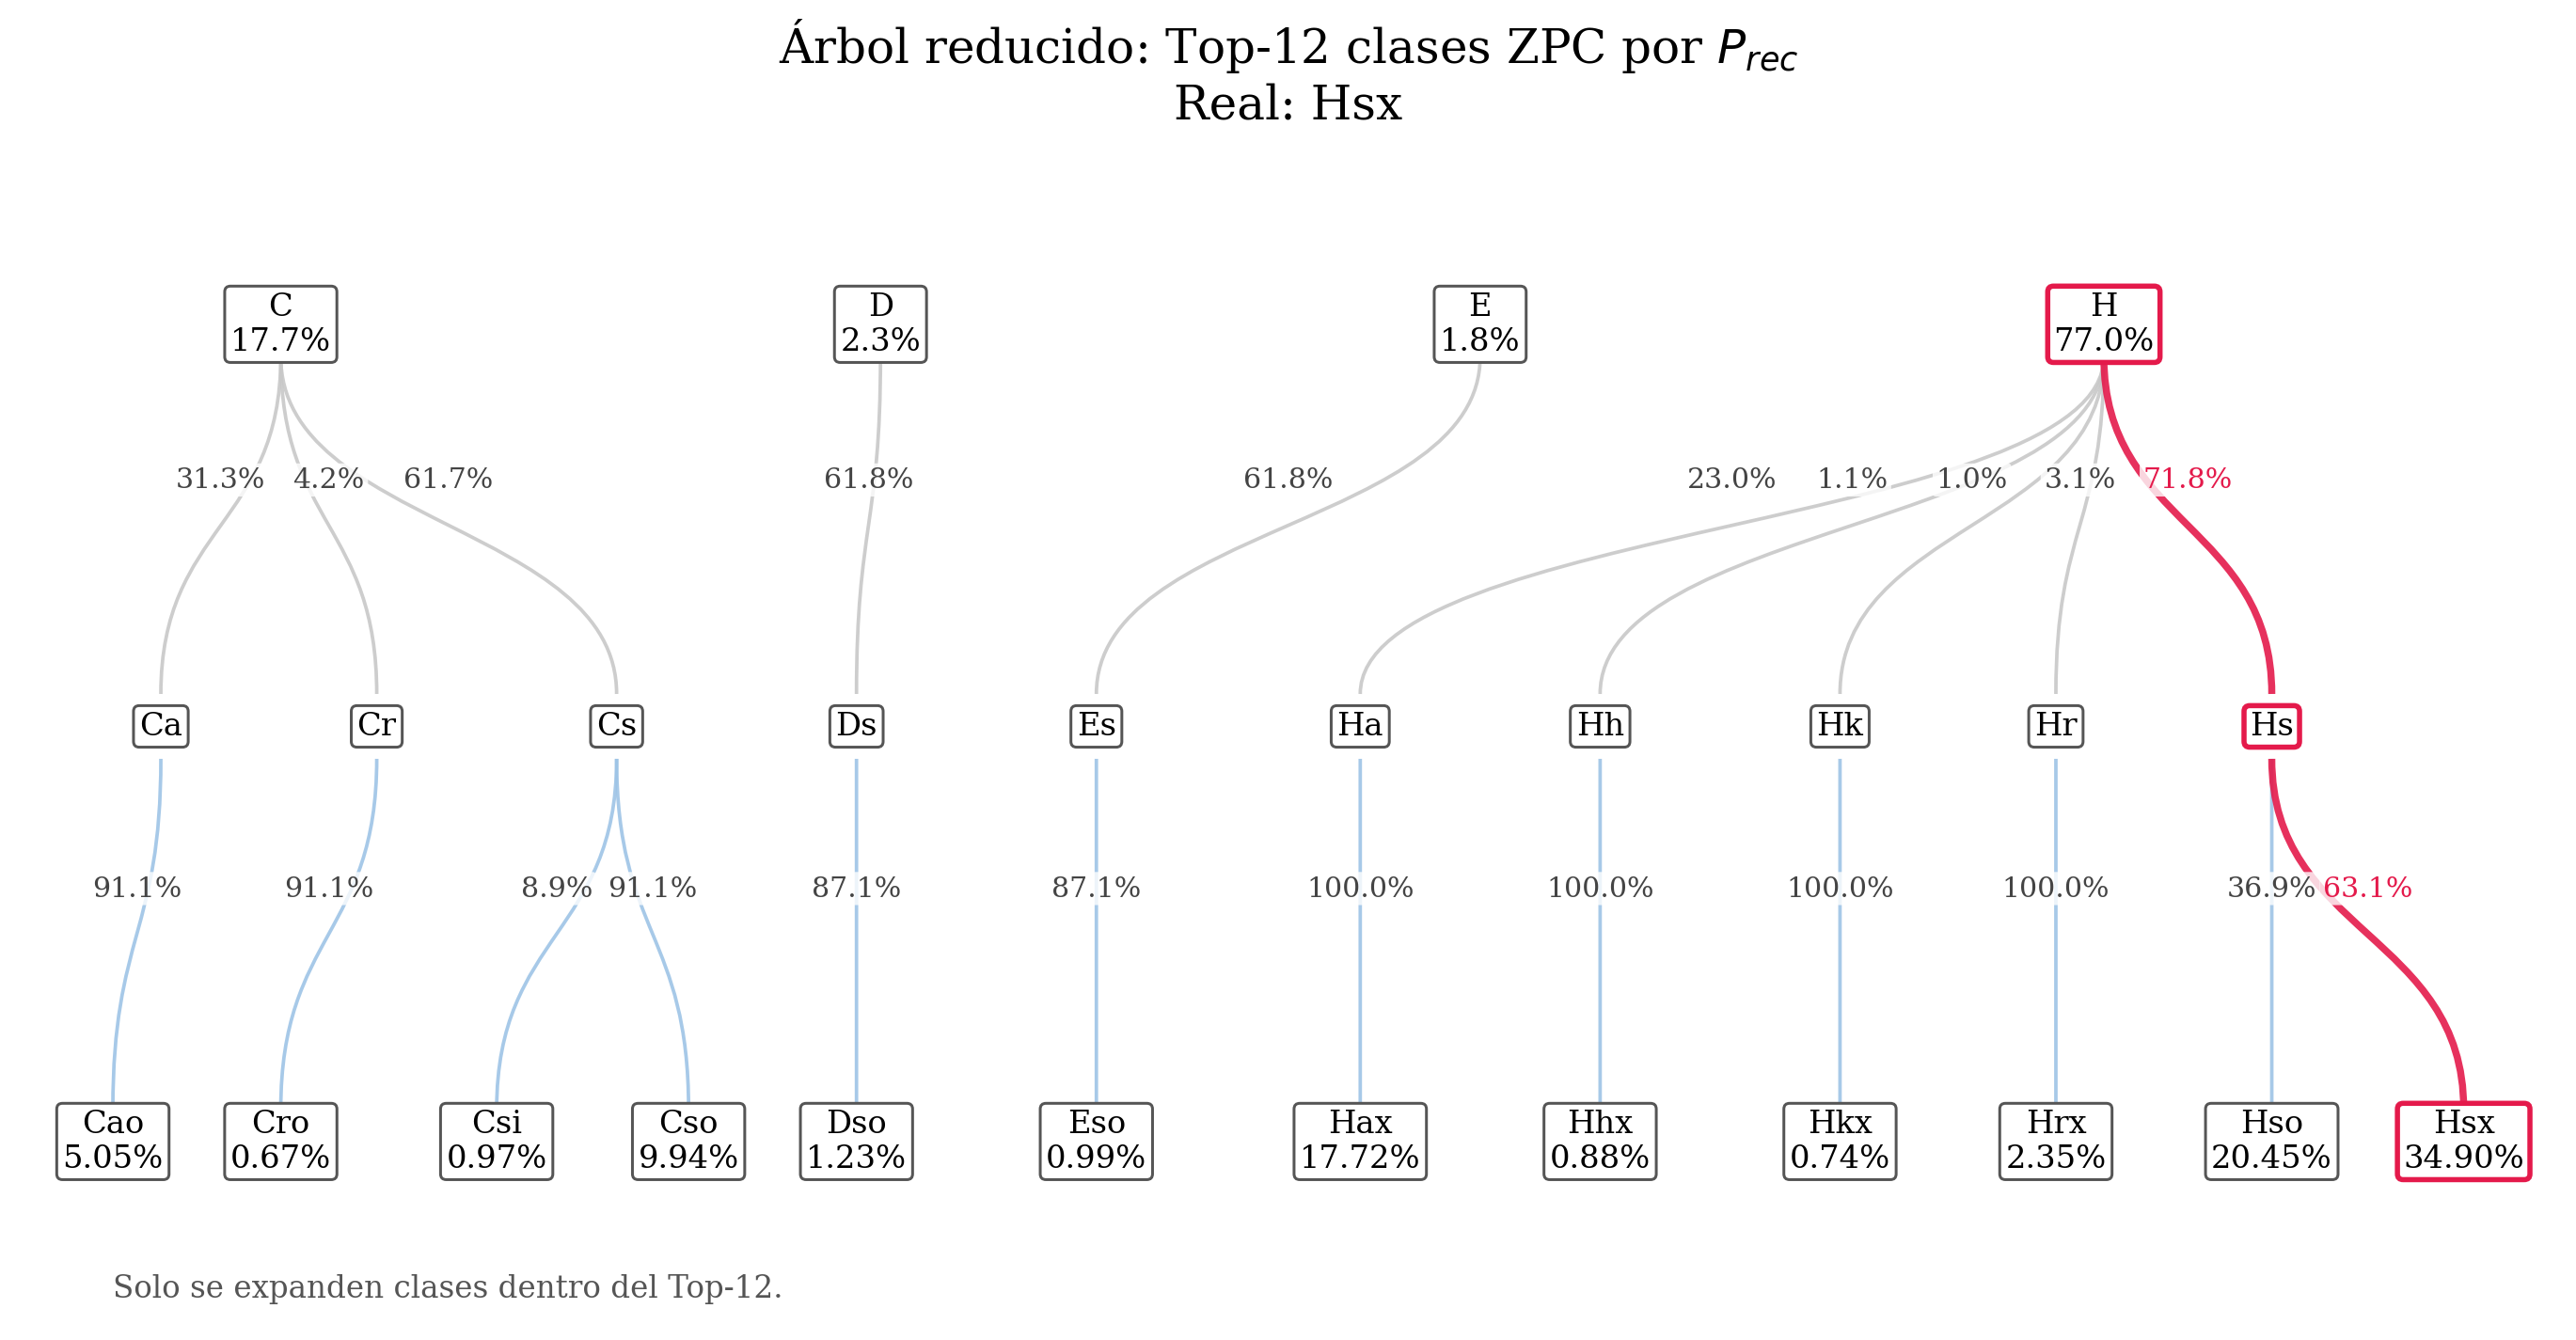
\includegraphics[height=0.85\textheight,width=0.96\linewidth,keepaspectratio]{ml/top12_tree.png}
    \vspace{0.08cm}
\end{frame}

\begin{frame}{Modelos de Deep Learning en Cascada: Árbol de recomendaciones semánticas}
    \centering
    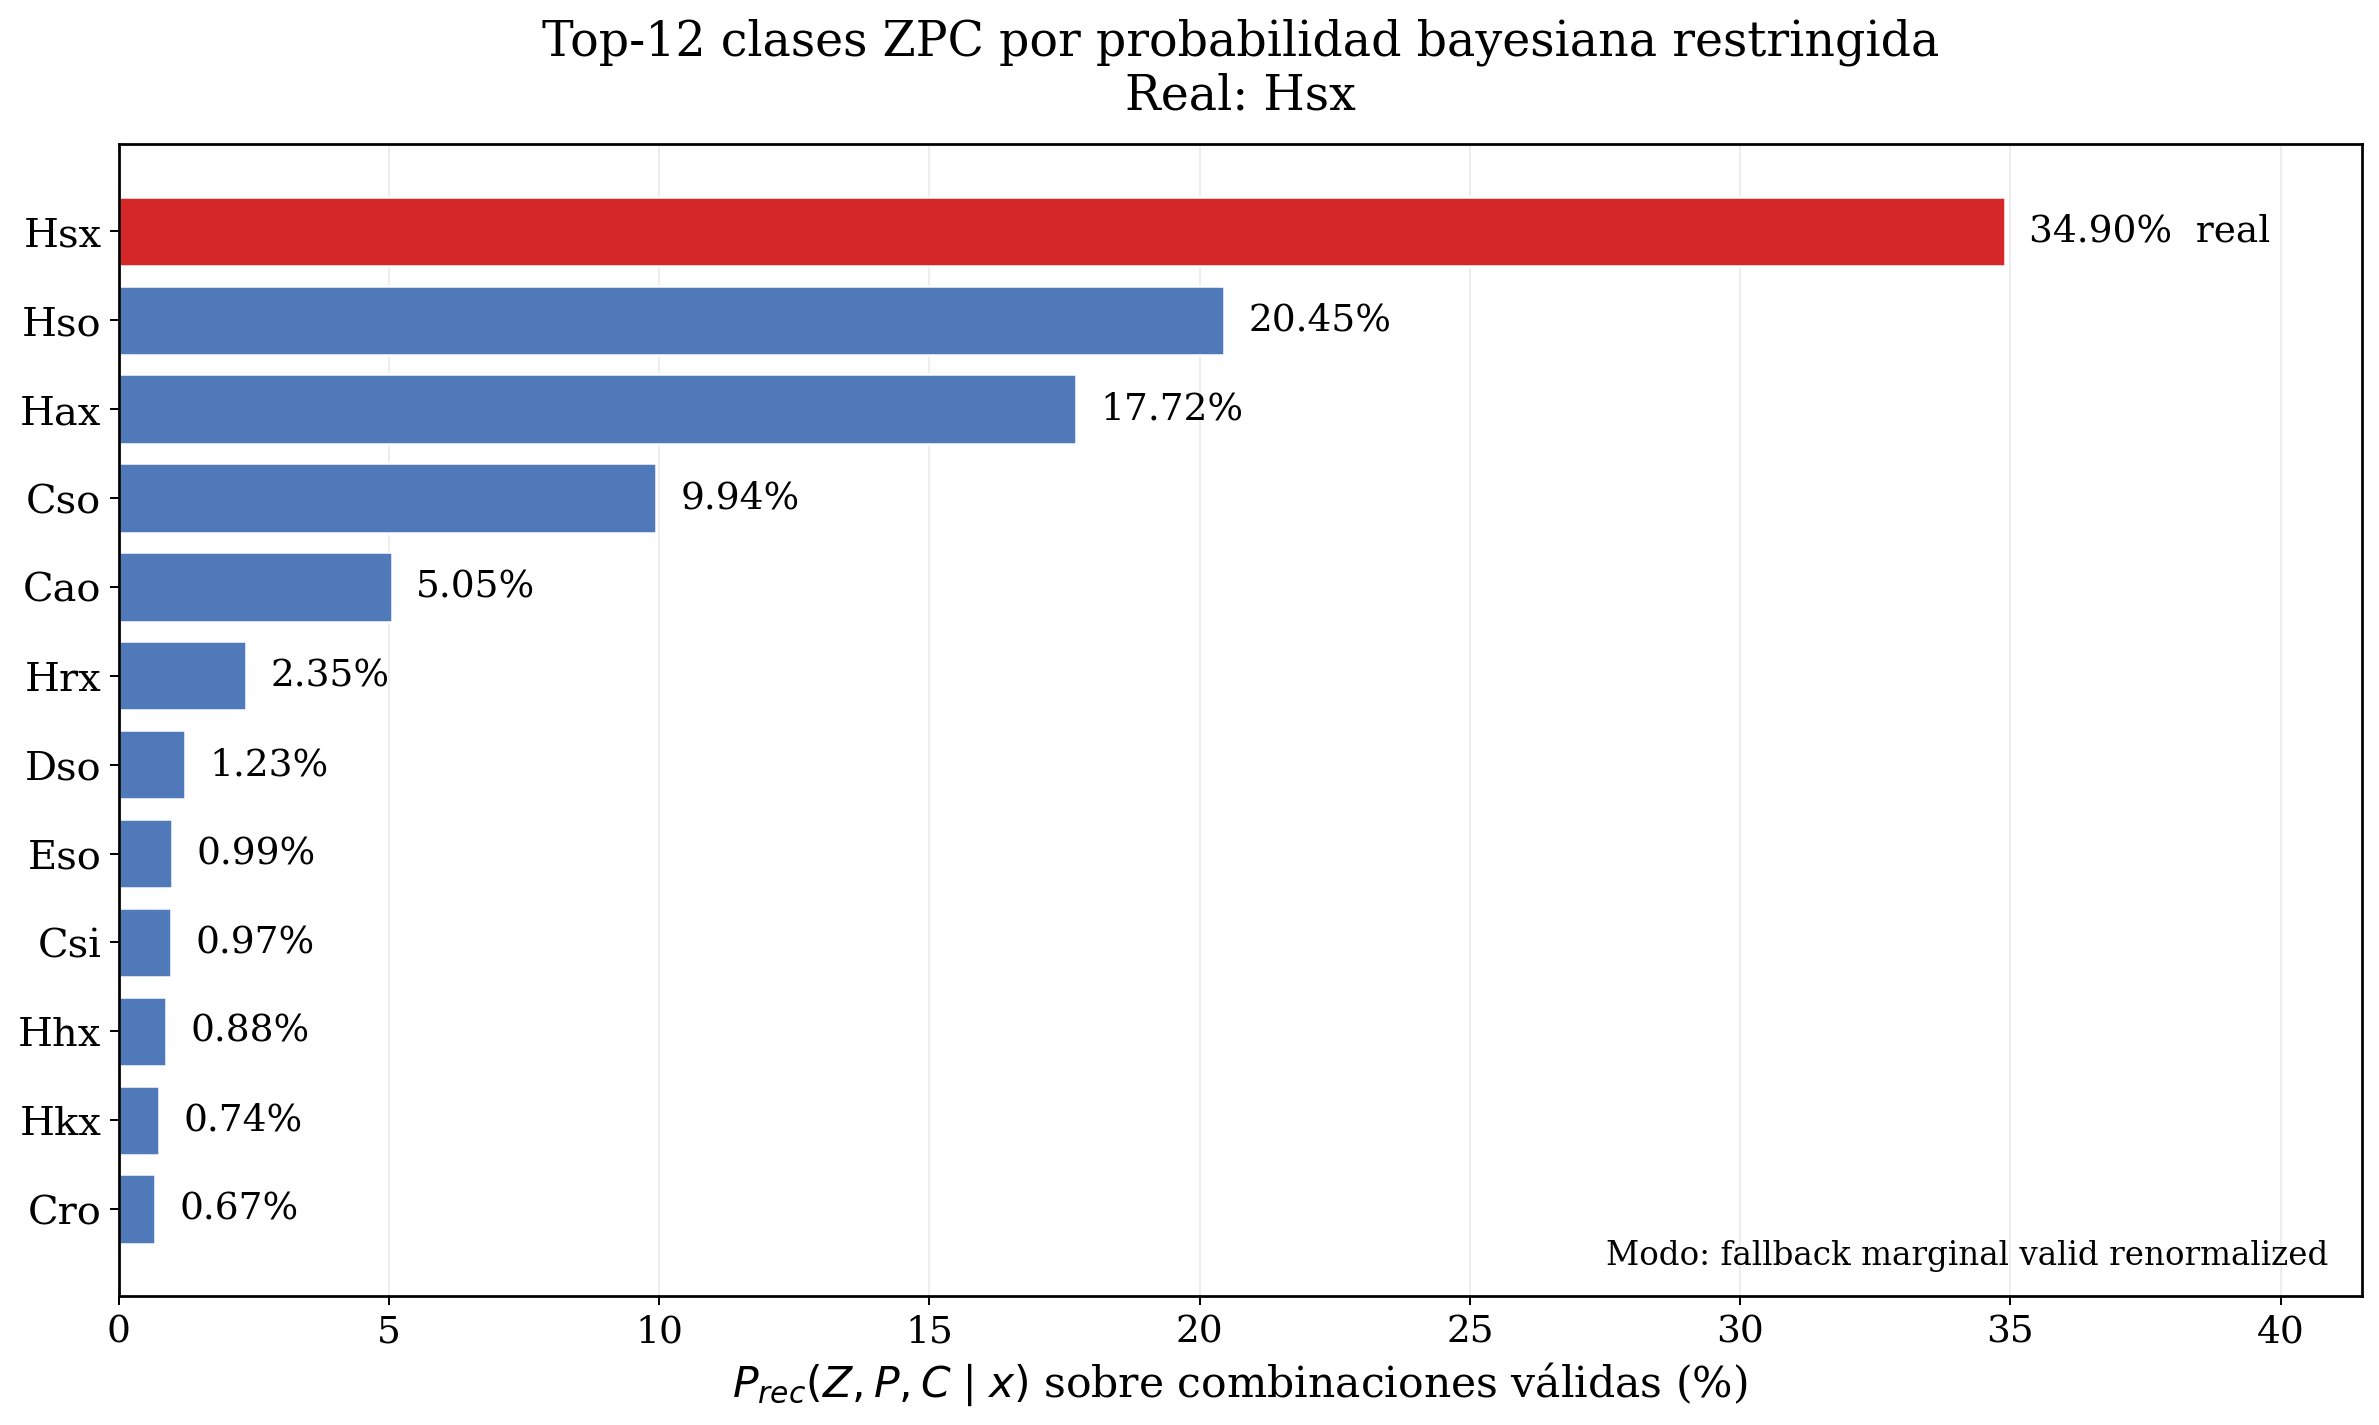
\includegraphics[height=0.82\textheight,width=0.96\linewidth,keepaspectratio]{ml/top12_rec.png}
    \vspace{0.08cm}
\end{frame}



% \begin{frame}{Estructura de Base de Datos (Supabase)}
%     \centering
%     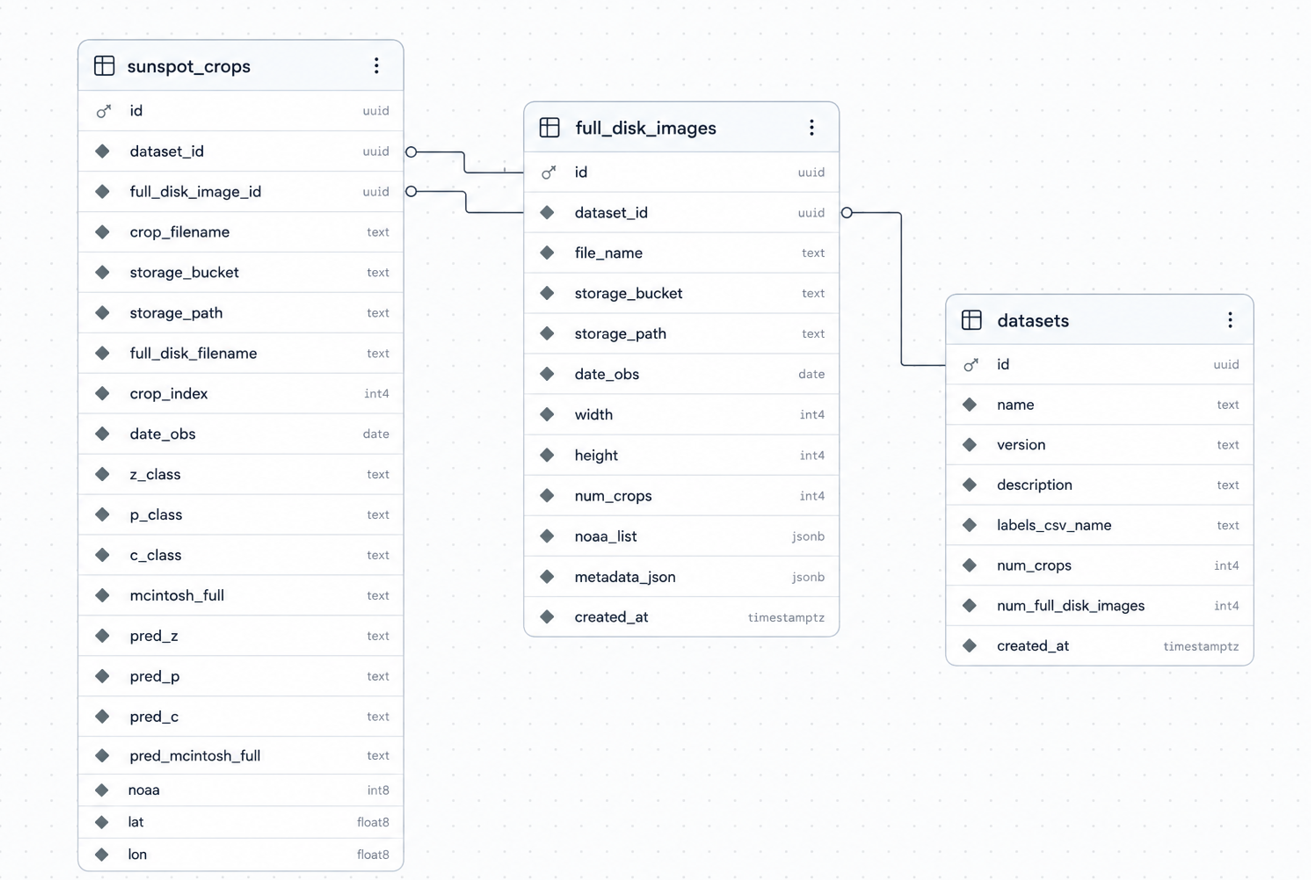
\includegraphics[height=0.82\textheight,width=0.96\linewidth,keepaspectratio]{data/db_schema.png}
%     \vspace{0.08cm}
% \end{frame}

\begin{frame}{Plataforma Web: Inicio}
    \vspace{-0.4cm} % Sube el recuadro para que quede alineado con el título
    
    % Envuelve el cuadro y lo empuja hacia el extremo derecho exacto
    \begin{columns}[t]
        \begin{column}{\textwidth}
            \hfill
            \setlength{\fboxrule}{1.2pt} % Grosor del borde
            \setlength{\fboxsep}{4pt}    % Margen interno del cuadro
            \fcolorbox{llamativoMagenta}{white}{%
                \scriptsize\textcolor{llamativoMagenta}{\textbf{Contribución 5}}
            }
        \end{column}
    \end{columns}
    \centering
    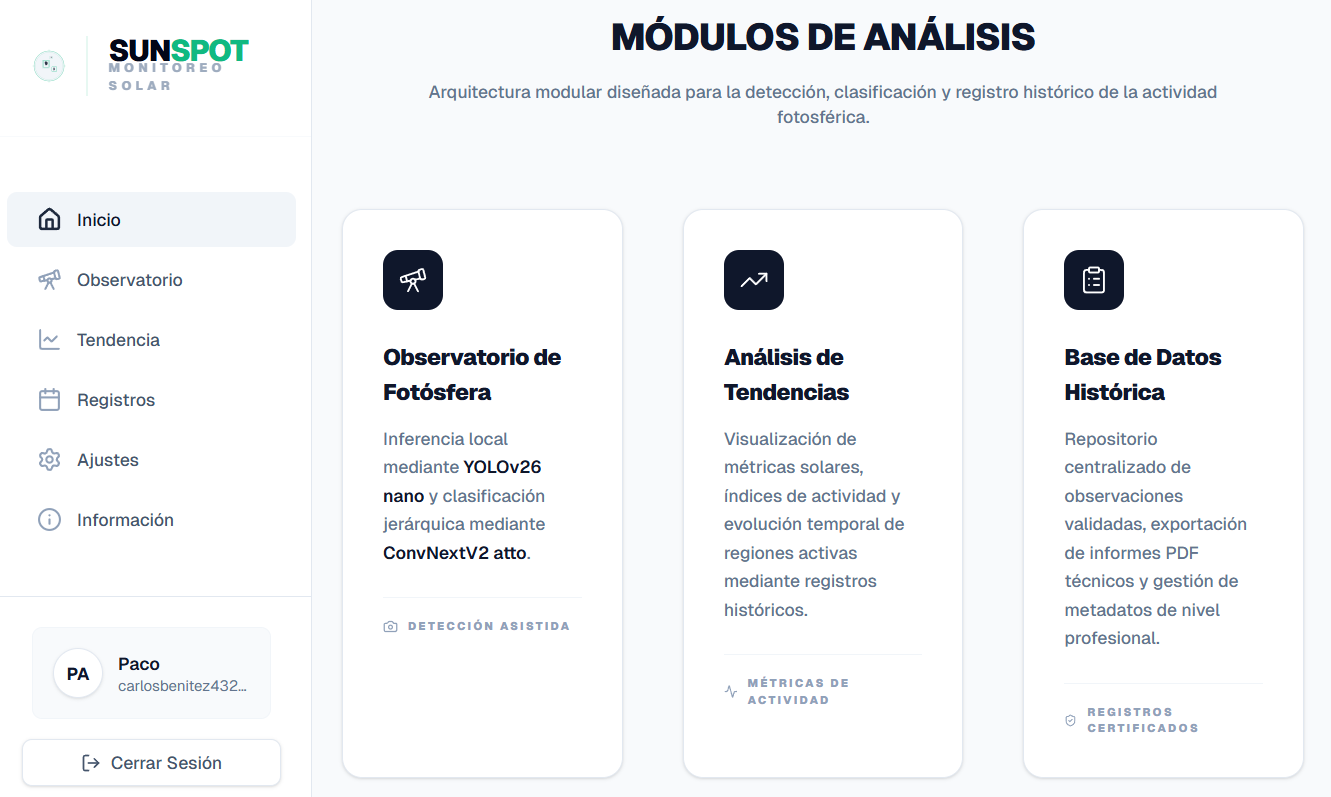
\includegraphics[height=0.75\textheight,width=0.96\linewidth,keepaspectratio]{web/home.png}
    \vspace{0.08cm}
\end{frame}

\begin{frame}{Plataforma Web: Carga de imagen}
    \centering
    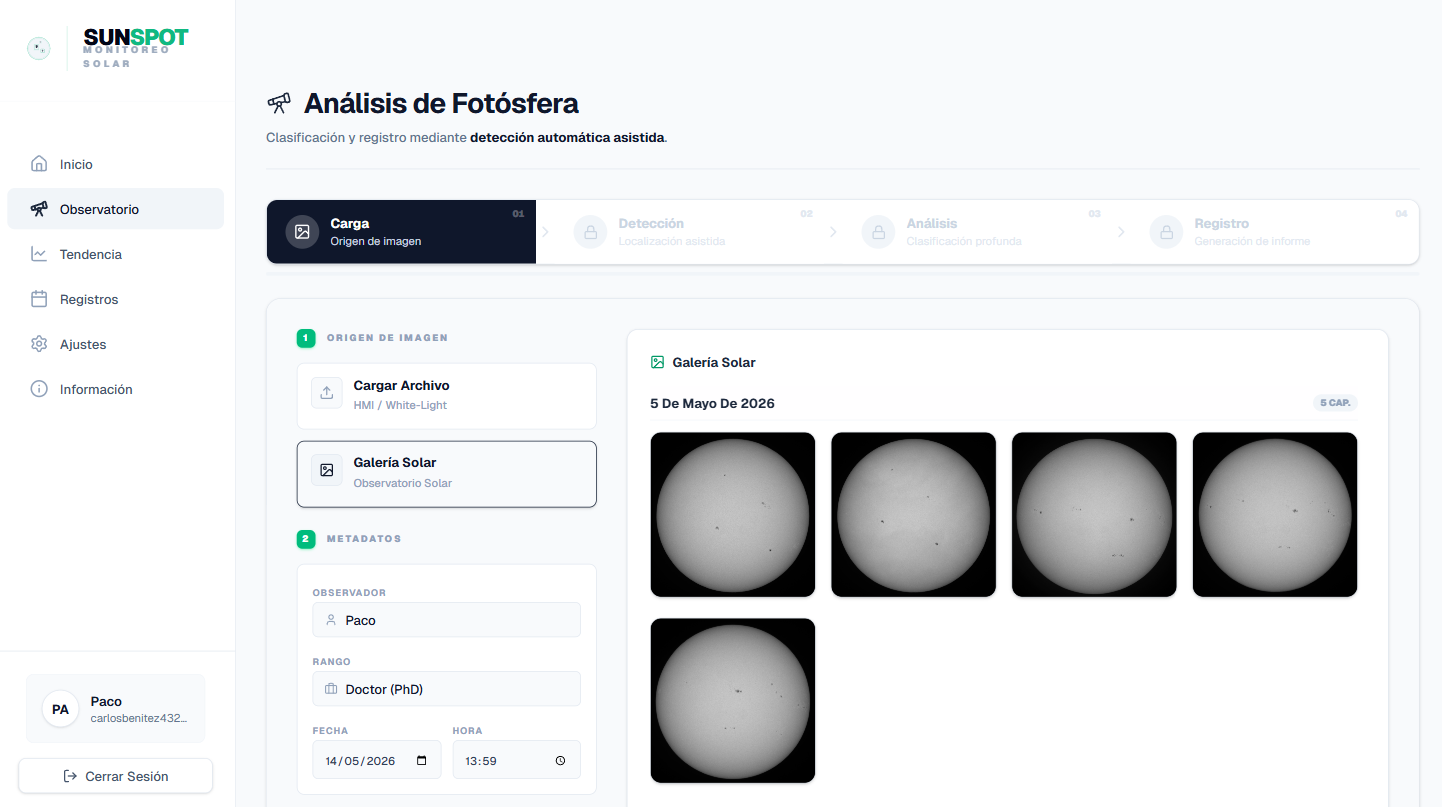
\includegraphics[height=0.75\textheight,width=0.96\linewidth,keepaspectratio]{web/upload.png}
    \vspace{0.08cm}
\end{frame}

\section{Resultados}

\begin{frame}{Resultados: Modelos de Detección y Clasificación}
    \vspace{-0.1cm}

    % --- Estructura Principal en Dos Columnas Grandes ---
    \begin{columns}[c, onlytextwidth]
        
        % Columna IZQUIERDA: Imagen completa con su respectivo Caption
        \begin{column}{0.40\textwidth}
            \begin{figure}
                \centering
                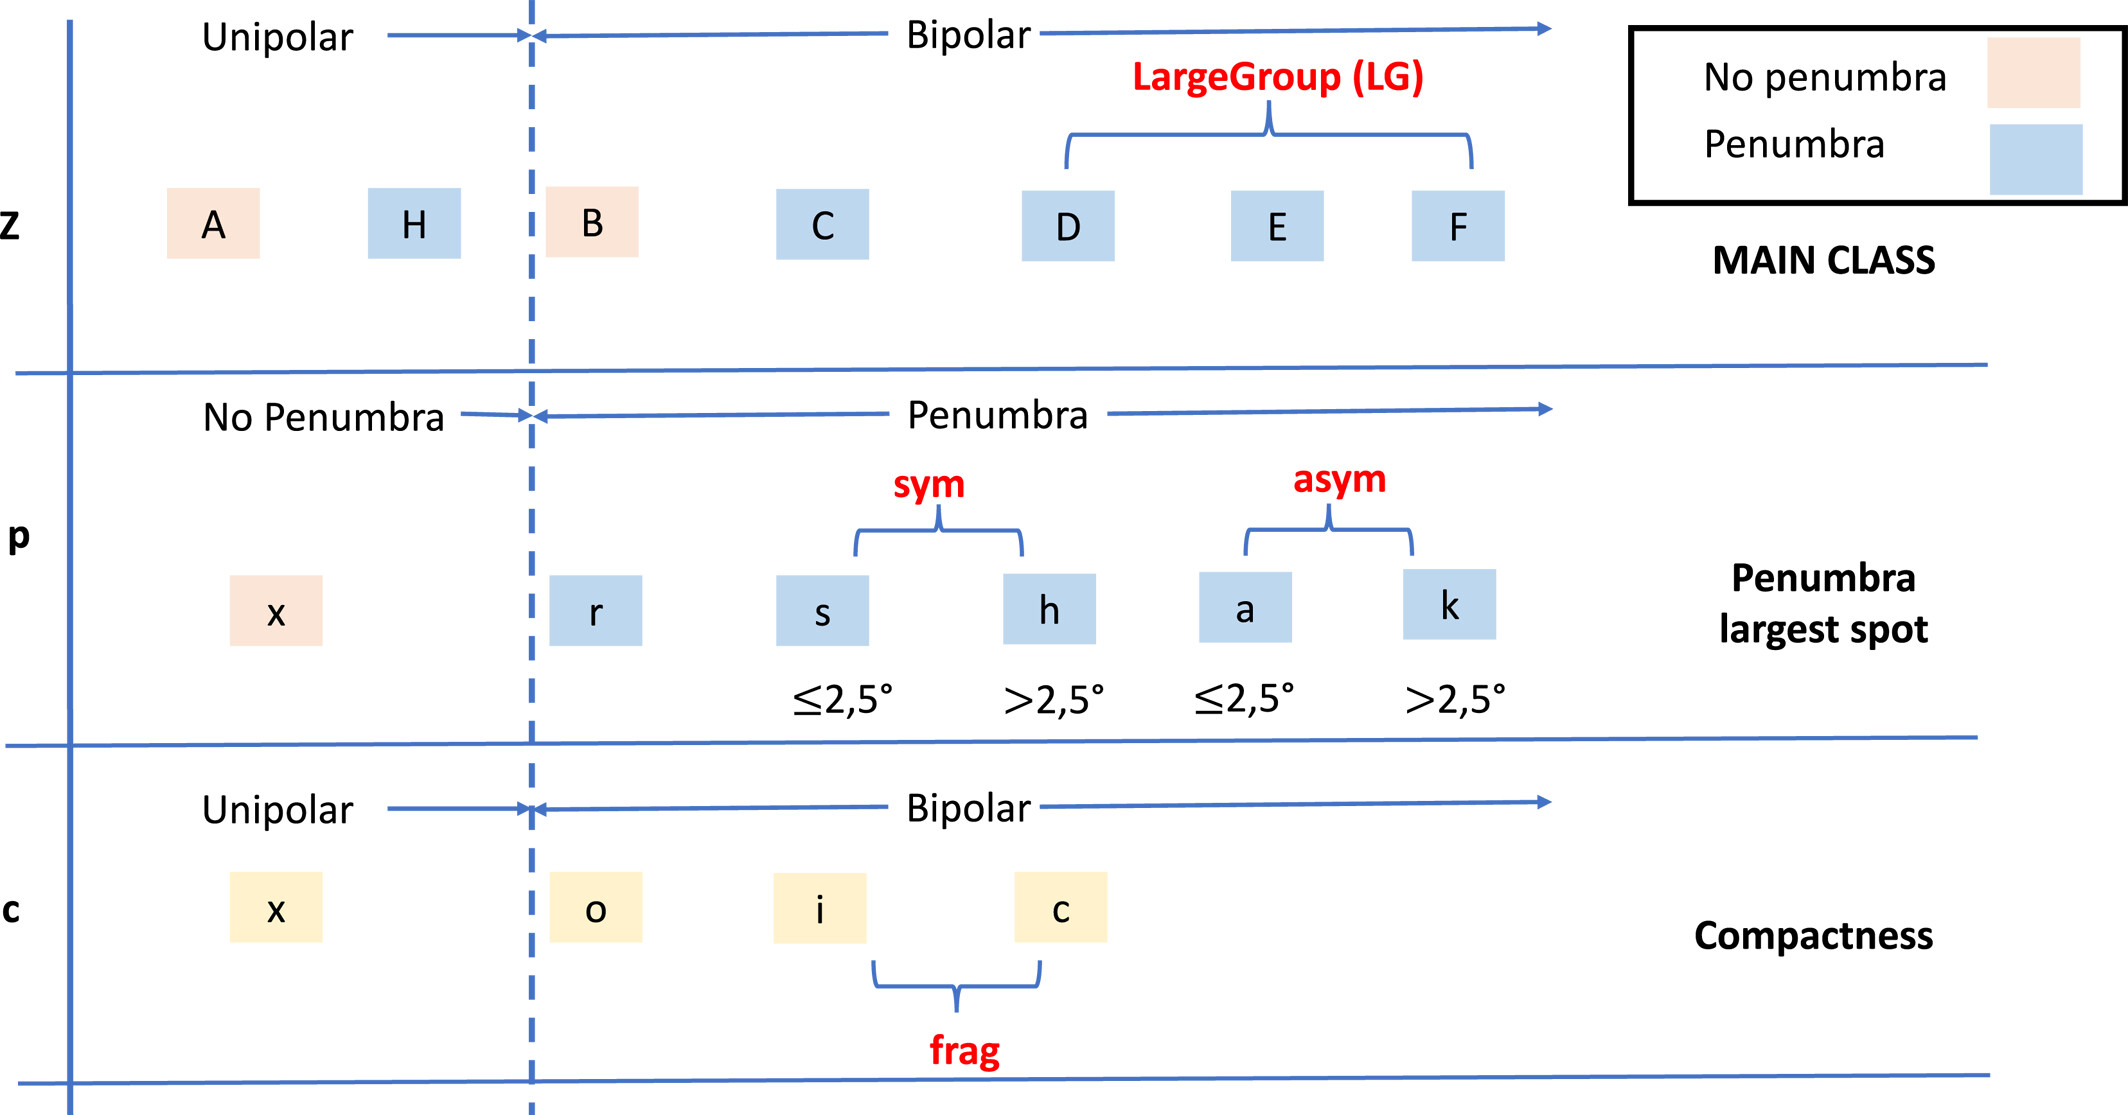
\includegraphics[height=0.58\textheight, width=\linewidth, keepaspectratio]{ref/sayezCompactacion.jpg}\par
                \vspace{0.05cm}
                {\scriptsize Compactación de clases en Sayez et al.}
            \end{figure}
        \end{column}
        
        \hfill
        
        % Columna DERECHA: Contiene la Tabla y justo debajo el Texto de Sayez
        \begin{column}{0.58\textwidth}
            \centering
            
            % 1. Tabla Comparativa Escalada y Compacta
            \renewcommand{\arraystretch}{1.1}
            \setlength{\tabcolsep}{4pt} 
            \begin{table}
                \scriptsize
                \centering
                \begin{tabular}{lcccc}
                    \toprule
                    \textbf{Autor} & \textbf{F1-Z} & \textbf{F1-P} & \textbf{F1-C} & \textbf{F1 p.} \\
                    \midrule
                    Palladino (2022) [15] & \textcolor{red!80!black}{\textbf{0.67}} & \textcolor{green!70!black}{0.55} & \textcolor{red!80!black}{\textbf{0.72}} & \textcolor{green!70!black}{0.65} \\
                    Sayez (2023) [4] & \textcolor{red!80!black}{\textbf{0.68}} & \textcolor{red!80!black}{\textbf{0.65}} & \textcolor{red!80!black}{\textbf{0.72}} & \textcolor{red!80!black}{\textbf{0.68}} \\
                    Deng (2025) [16] & \textcolor{green!70!black}{0.47} & \textcolor{green!70!black}{0.41} & \textcolor{green!70!black}{0.60} & \textcolor{green!70!black}{0.49} \\
                    
                    % Fila de la propuesta con celdas pintadas individualmente y texto en blanco para alto contraste
                    \cellcolor{llamativoMagenta}\textcolor{white}{\textbf{Propuesta}} & 
                    \cellcolor{llamativoMagenta}\textcolor{white}{\textbf{0.65}} & 
                    \cellcolor{llamativoMagenta}\textcolor{white}{\textbf{0.63}} & 
                    \cellcolor{llamativoMagenta}\textcolor{white}{\textbf{0.71}} & 
                    \cellcolor{llamativoMagenta}\textcolor{white}{\textbf{0.66}} \\
                    \bottomrule
                \end{tabular}
            \end{table}

            \vspace{0.15cm}

            \scriptsize
            Sayez et al. (2023) agrupa las clases de algunos caracteres por lo que es de esperarse la mejoría en las métricas; sin embargo, este ajuste rompe la operatividad del modelo ya que introduce una clasificación distinta.
            
        \end{column}
        
    \end{columns}

    \vfill

    % --- Bloque de Referencias Unificado y Compacto ---
    {\tiny\color{gray}
    [4] M. Sayez et al., “SunSCC: Automated solar classification dataset,” Astronomy \& Astrophysics, 2023. \par\vspace{0.03cm}
    [15] L. Palladino, E. Ntagiou, J. Klug, J. Palacios, y R. Keil, “Sunspot groups detection and classification on SDO/HMI images using deep learning techniques,” in 2022 IEEE Aerospace Conference. IEEE, 2022, pp. 1–10. \par\vspace{0.03cm}
    [16] X. Deng et al., “Deep learning-based McIntosh classification of sunspotgroups,” Astronomy and Computing, vol. 53, p. 100995, 2025.\par}
\end{frame}

\begin{frame}{Resultados: Modelos Predictivos}
    \centering
    \small

    % Primera Tabla: Métricas Vectoriales (Valores reales extraídos del documento)
    \scriptsize \textbf{Resultados del DMD-Spörer (Vectorial)}
    \renewcommand{\arraystretch}{1.2}
    \begin{table}
        \centering
        \scriptsize
        \begin{tabular}{l|l|c}
            \toprule
            \textbf{Métrica} & \textbf{Descripción} & \textbf{DMD-Spörer} \\ 
            \midrule
            $\textstyle E_F = \frac{\|\mathbf{X}-\widehat{\mathbf{X}}\|_F}{\|\mathbf{X}\|_F}$ & Error de Frobenius (Fidelidad global) & 0.4087 \\
            $\textstyle \rho_{ST} = \operatorname{corr}(\operatorname{vec}(\mathbf{X}),\operatorname{vec}(\widehat{\mathbf{X}}))$ & Correlación spatio-temporal & 0.9126 \\
            $\textstyle \mathrm{MLCE} = \frac{1}{N}\sum_{t=1}^{N}|\theta_c(t)-\widehat{\theta}_c(t)|$ & Error latitud central & 1.25$^\circ$ \\ 
            \bottomrule
        \end{tabular}
    \end{table}

    \vspace{0.05cm}

    % Segunda Tabla: Métricas Escalares (Valores reales extraídos del documento)
    \scriptsize \textbf{Resultados de PVLK y DMD-Spörer (Escalar)}
    \renewcommand{\arraystretch}{1.2}
    \begin{table}
        \centering
        \scriptsize
        \begin{tabular}{l|l|cc}
            \toprule
            \textbf{Métrica} & \textbf{Descripción} & $\text{\textbf{SSN}}_{\text{\textbf{PVLK}}}$ & $\text{\textbf{SSN}}_{\text{\textbf{DMD}}}$ \\ 
            \midrule
            $\textstyle \mathrm{MAE} = \frac{1}{N}\sum_{k=1}^{N}|z_k-\widehat{s}_k|$ & Error absoluto medio & 15.31 & 15.22 \\
            $\textstyle \mathrm{RMSE} = \sqrt{\frac{1}{N}\sum_{k=1}^{N}(z_k-\widehat{s}_k)^2}$ & Error cuadrático medio & 22.02 & 20.30 \\
            $\textstyle \mathrm{MAPE} = \frac{100}{N}\sum_{k=1}^{N}\left|\frac{z_k-\widehat{s}_k}{z_k}\right|$ & Error porcentual medio & 33.27\% & 32.54\% \\
            $\textstyle R^2 = 1-\frac{\sum_k(z_k-\widehat{s}_k)^2}{\sum_k(z_k-\bar{z})^2}$ & Coeficiente de determinación & 0.8173 & 0.8449 \\
            \bottomrule
        \end{tabular}
    \end{table}

\end{frame}

\begin{frame}{Resultados: Adquisición y nodo local}
    \small
    \vspace{-0.1cm}
    
    \begin{columns}[c] % <--- Centrado vertical global para las columnas
        
        % COLUMNA IZQUIERDA: Imagen Dominante
        \begin{column}[c]{0.55\textwidth} % <--- Centrado vertical individual
            \centering
            \textbf{Captura solar registrada el 2026-05-05}\\[0.1cm]
            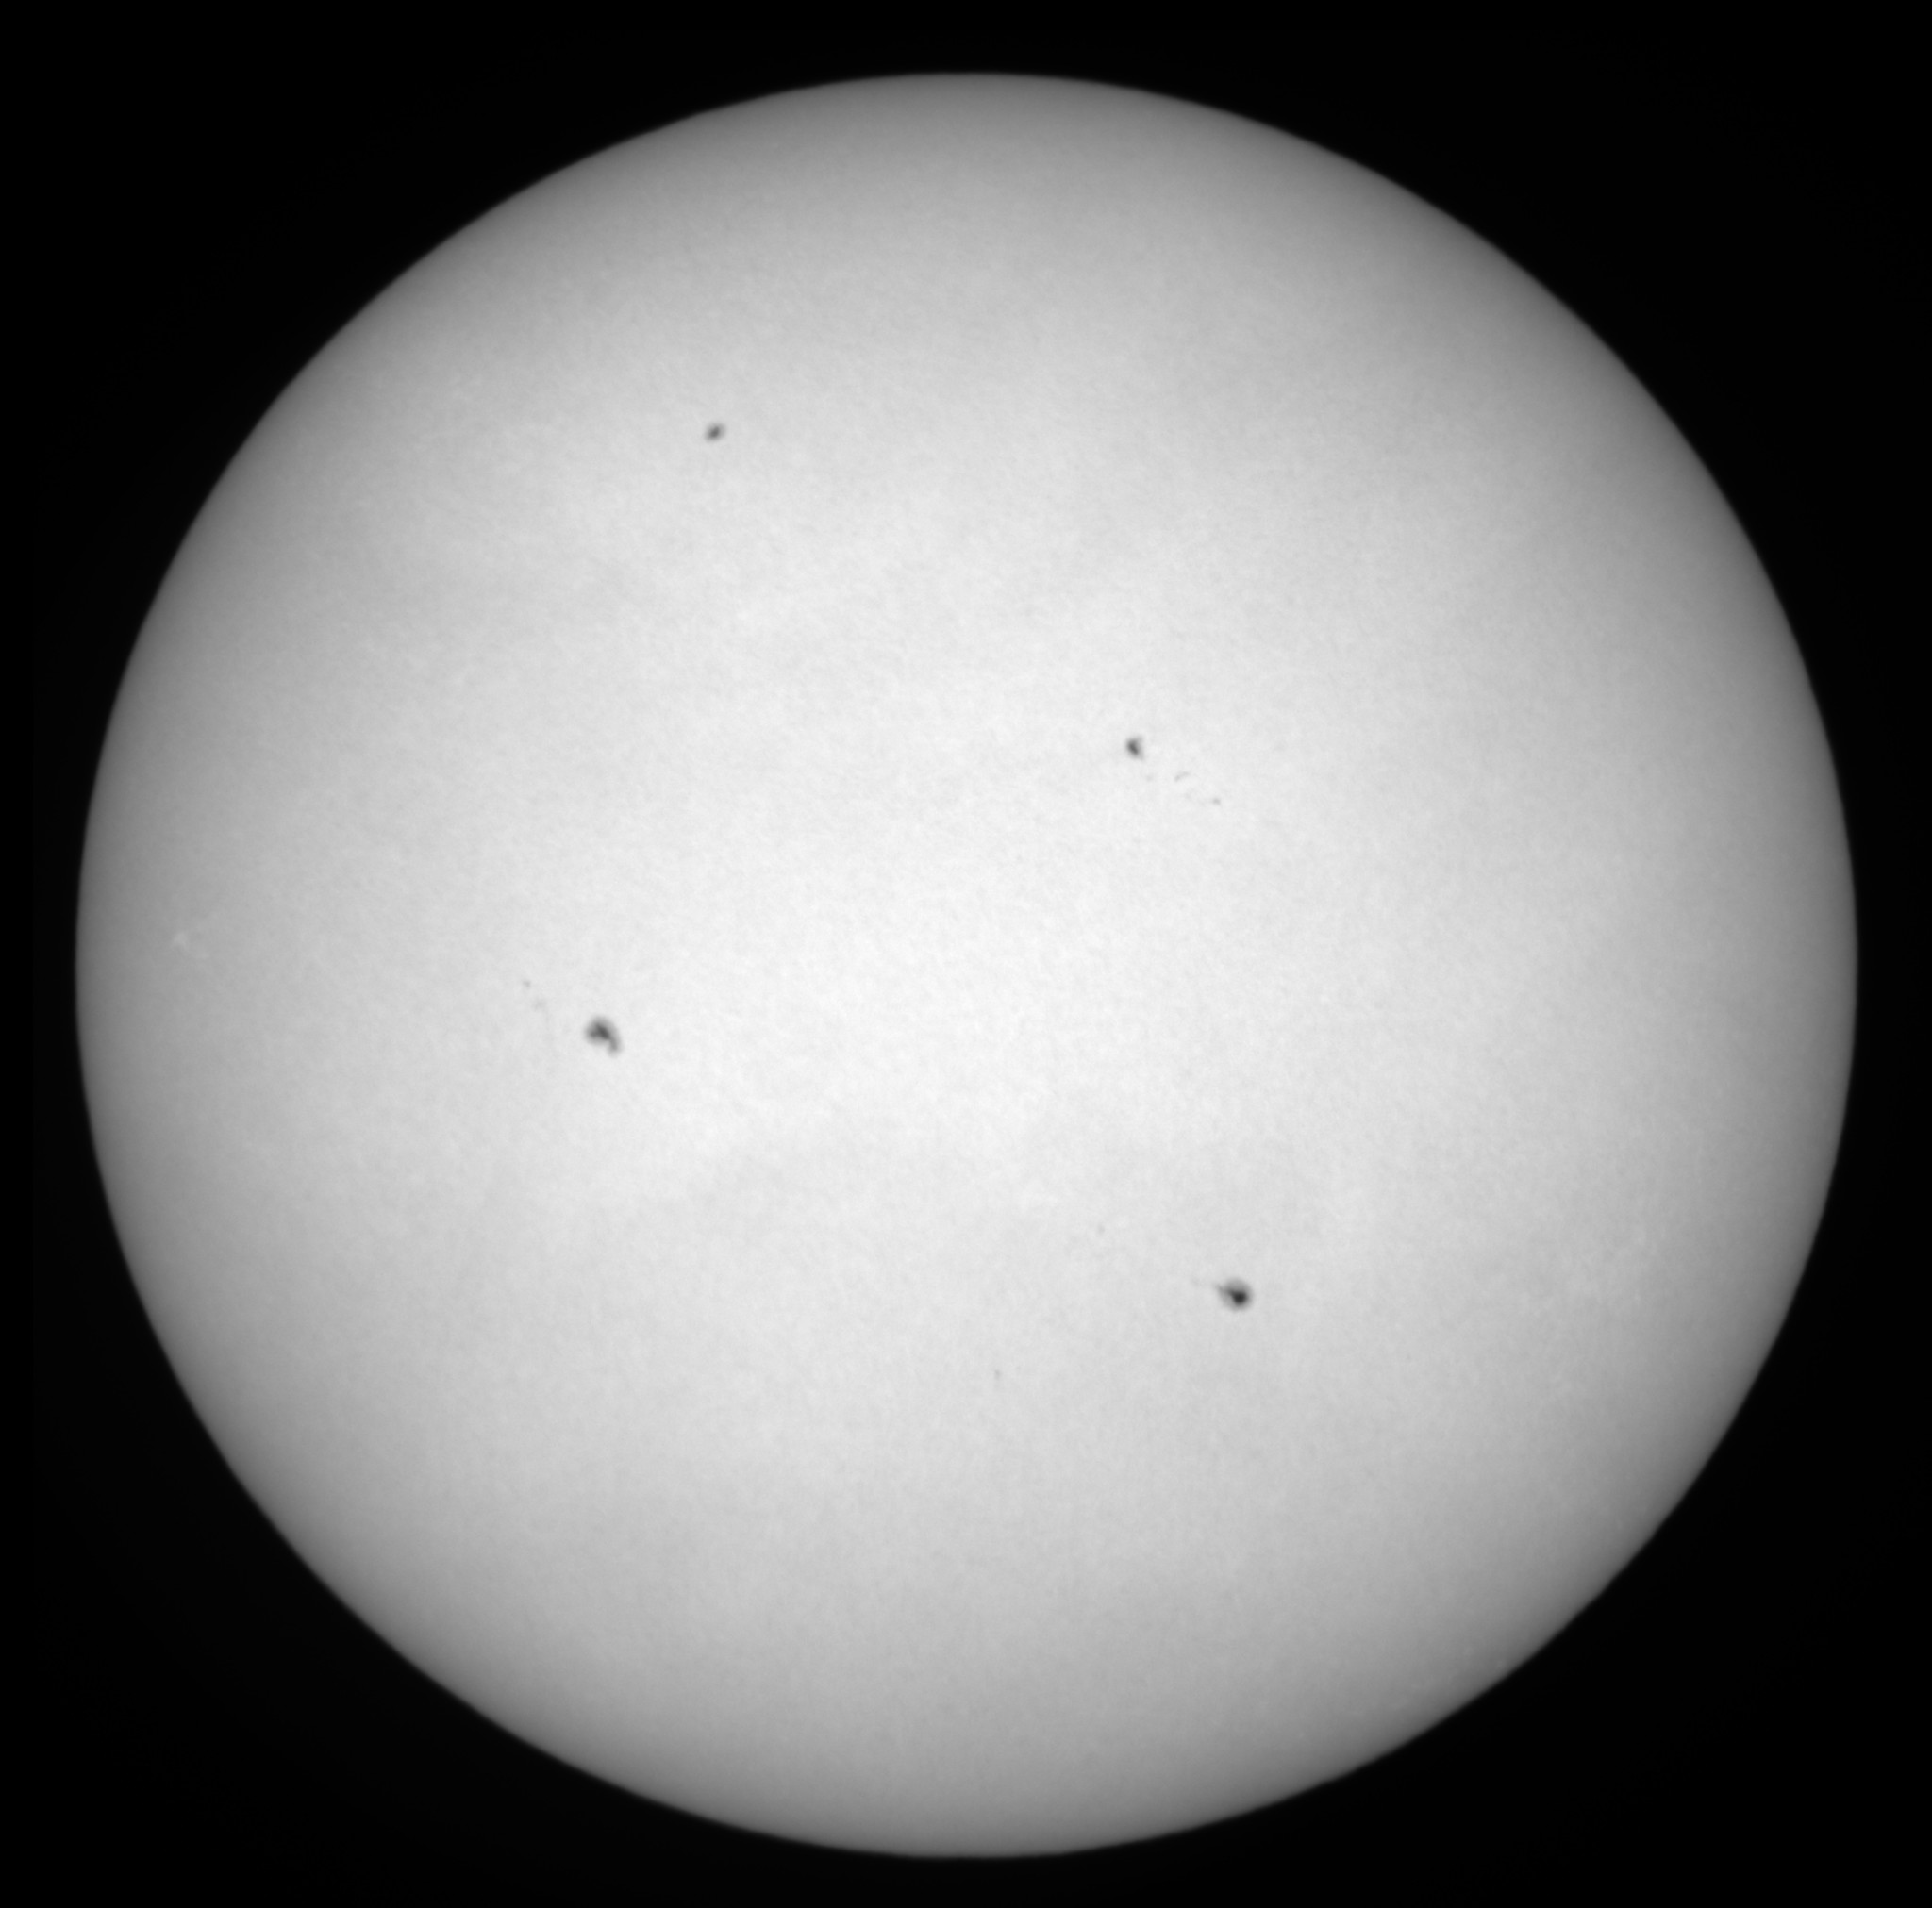
\includegraphics[width=0.95\textwidth, height=6.0cm, keepaspectratio]{obs/capture.jpg} 
        \end{column}
        
        % COLUMNA DERECHA: Ambas tablas centradas respecto a la imagen
        \begin{column}[c]{0.42\textwidth} % <--- Centrado vertical individual
            \centering
            
            % Primera Tabla: Adquisición
            \scriptsize \textbf{Adquisición}\\[0.05cm]
            \renewcommand{\arraystretch}{1.0} 
            \begin{tabular}{lc}
                \toprule
                \textbf{Parámetro} & \textbf{Valor} \\
                \midrule
                Formato & FITS / RGB24 \\
                Resolución & 1936 $\times$ 1216 px \\
                FPS / Exposición & 15 / 500 $\mu$s \\
                \bottomrule
            \end{tabular}
            
            \vspace{0.4cm} % Un toque más de separación para balancear el bloque
            
            % Segunda Tabla: Raspberry Pi 5
            \textbf{Raspberry Pi 5}\\[0.05cm]
            \begin{tabular}{lc}
                \toprule
                \textbf{Métrica} & \textbf{Valor} \\
                \midrule
                Captura + Guardado & 600 ms \\
                Preprocesamiento & 1350 ms \\
                Sincronización & 3800 ms/img \\
                CPU medio/máx. & 38\% / 72\% \\
                RAM / Temp. 25 min & 3.3 GB / 57 $^{\circ}$C \\
                \bottomrule
            \end{tabular}
        \end{column}
        
    \end{columns}
\end{frame}


\begin{frame}{Resultado de Campo: Plataforma Web (Detección con YOLO26n ONNX)}
    \centering
    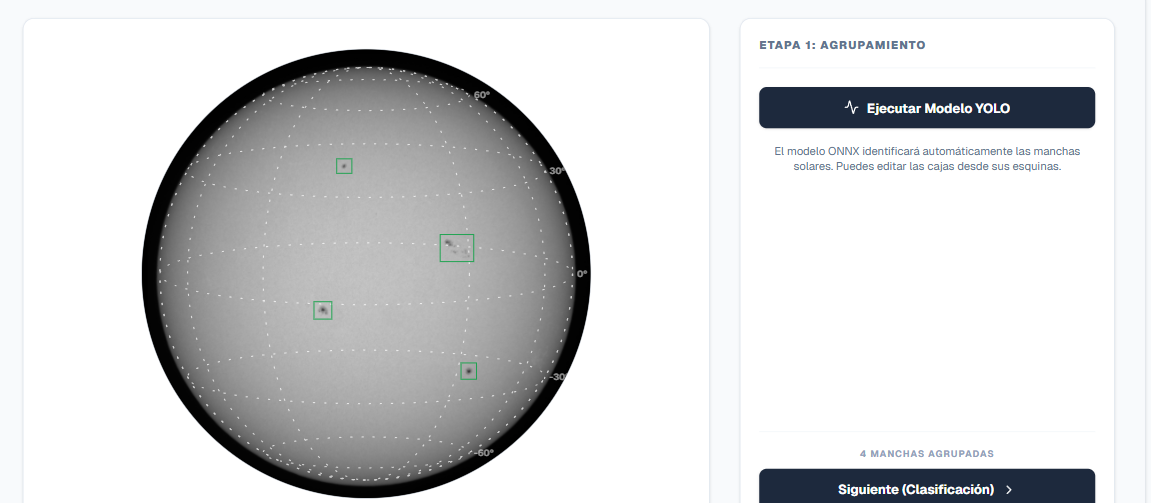
\includegraphics[height=0.75\textheight,width=0.96\linewidth,keepaspectratio]{web/yolo.png}
    \vspace{0.08cm}
\end{frame}

\begin{frame}{Resultados: Plataforma Web (Clasificación con modelo jerárquica ConvNeXtv2a ONNX)}
    \centering
    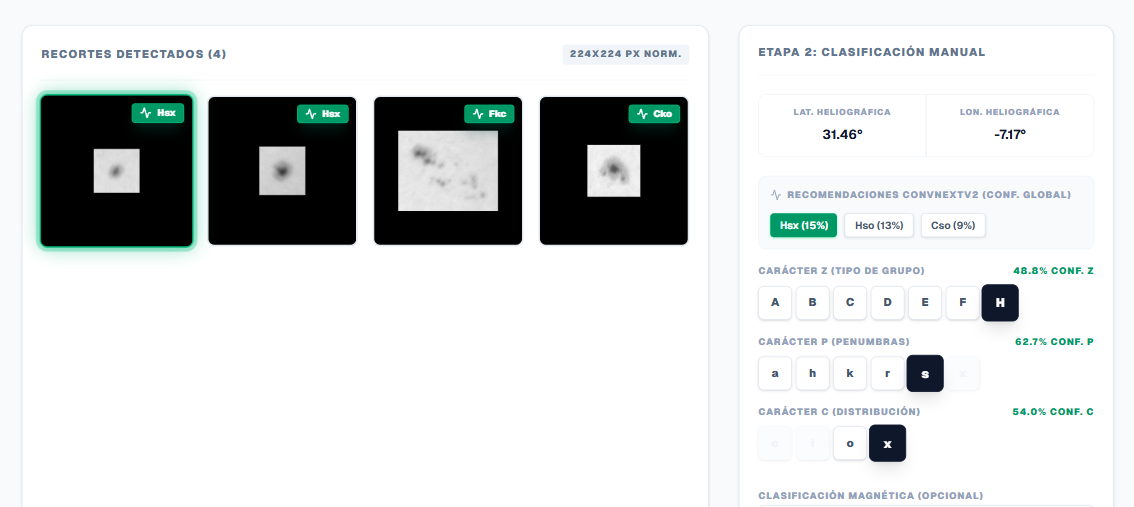
\includegraphics[height=0.75\textheight,width=0.96\linewidth,keepaspectratio]{web/convnext.png}
    \vspace{0.08cm}
\end{frame}

\begin{frame}{Resultados: Plataforma Web (Diagrama de Spörer)}
    \centering
    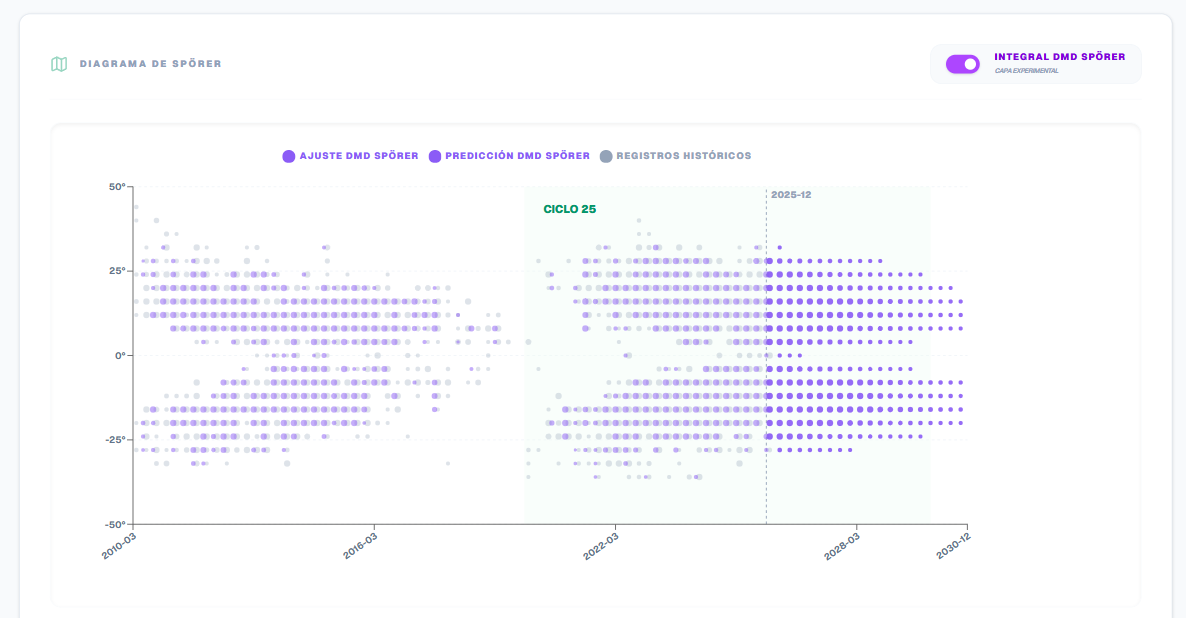
\includegraphics[height=0.75\textheight,width=0.96\linewidth,keepaspectratio]{web/butterfly.png}
    \vspace{0.08cm}
\end{frame}

\begin{frame}{Resultados: Plataforma Web (Predicción SSN)}
    \centering
    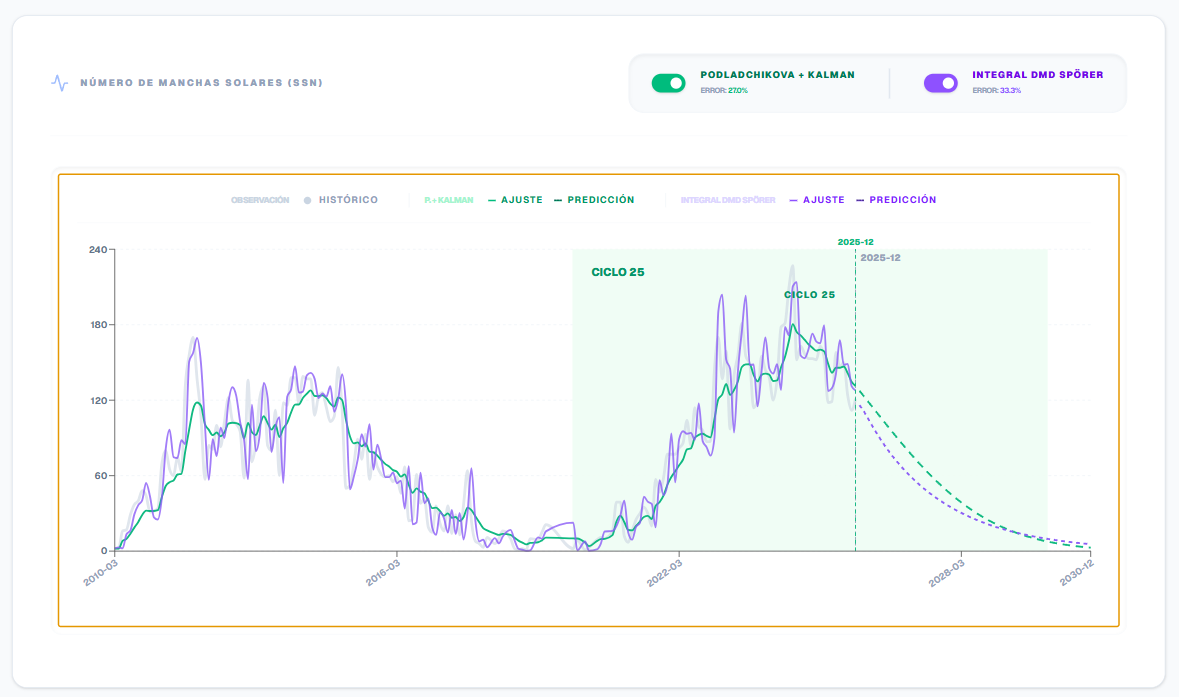
\includegraphics[height=0.75\textheight,width=0.96\linewidth,keepaspectratio]{web/ssn.png}
    \vspace{0.08cm}
\end{frame}


\section{Conclusiones}

\begin{frame}{Conclusiones}
    \small
    
     La articulación de los componentes de hardware y software permite extraer las siguientes conclusiones:
    
    \begin{itemize}
        \scriptsize
        \item \textbf{Autonomía:} El dispositivo de adquisición local permite el flujo de datos sin dependencia de conectividad externa constante.
        \item \textbf{Procesamiento en el borde (ONNX):} La integración de modelos basados en DMD y \textit{Deep Learning} valida la viabilidad técnica de ejecutar tareas de clasificación y análisis predictivo en entornos locales.
        \item \textbf{Monitoreo:} El \textit{framework} operativo unifica la captura y el análisis automatizado de forma desacoplada.
    \end{itemize}

    \centering
    
    % Tabla de correspondencia con los objetivos específicos (OE)
    \renewcommand{\arraystretch}{1.2} 
    \begin{table}
        \centering
        \scriptsize
        \begin{tabular}{l|l|c}
            \toprule
            \textbf{Identificador} & \textbf{Descripción de la Contribución} & \textbf{Vínculo} \\ 
            \midrule
            \contrib{Contribución 1} & Dispositivo de Adquisición local autónomo & $\text{OE}_2$, $\text{OE}_6$ \\ 
            \contrib{Contribución 2} & Base de datos etiquetada de actividad solar & $\text{OE}_1$, $\text{OE}_2$ \\ 
            \contrib{Contribución 3} & Modelo del Diagrama de Spörer basado en DMD & $\text{OE}_4$ \\ 
            \contrib{Contribución 4} & Modelo jerárquico de Deep Learning (Clasificación) & $\text{OE}_3$ \\ 
            \contrib{Contribución 5} & Framework de observación asistida & $\text{OE}_5$, $\text{OE}_6$ \\ 
            \bottomrule
        \end{tabular}
    \end{table}
\end{frame}


\begin{frame}{Trabajo futuro y recomendaciones metodológicas}
    \begin{columns}[c] % Alineación vertical centrada de las columnas
        
        % Columna Izquierda: Imagen del equipo/telescopio
        \begin{column}{0.40\textwidth}
            \centering
            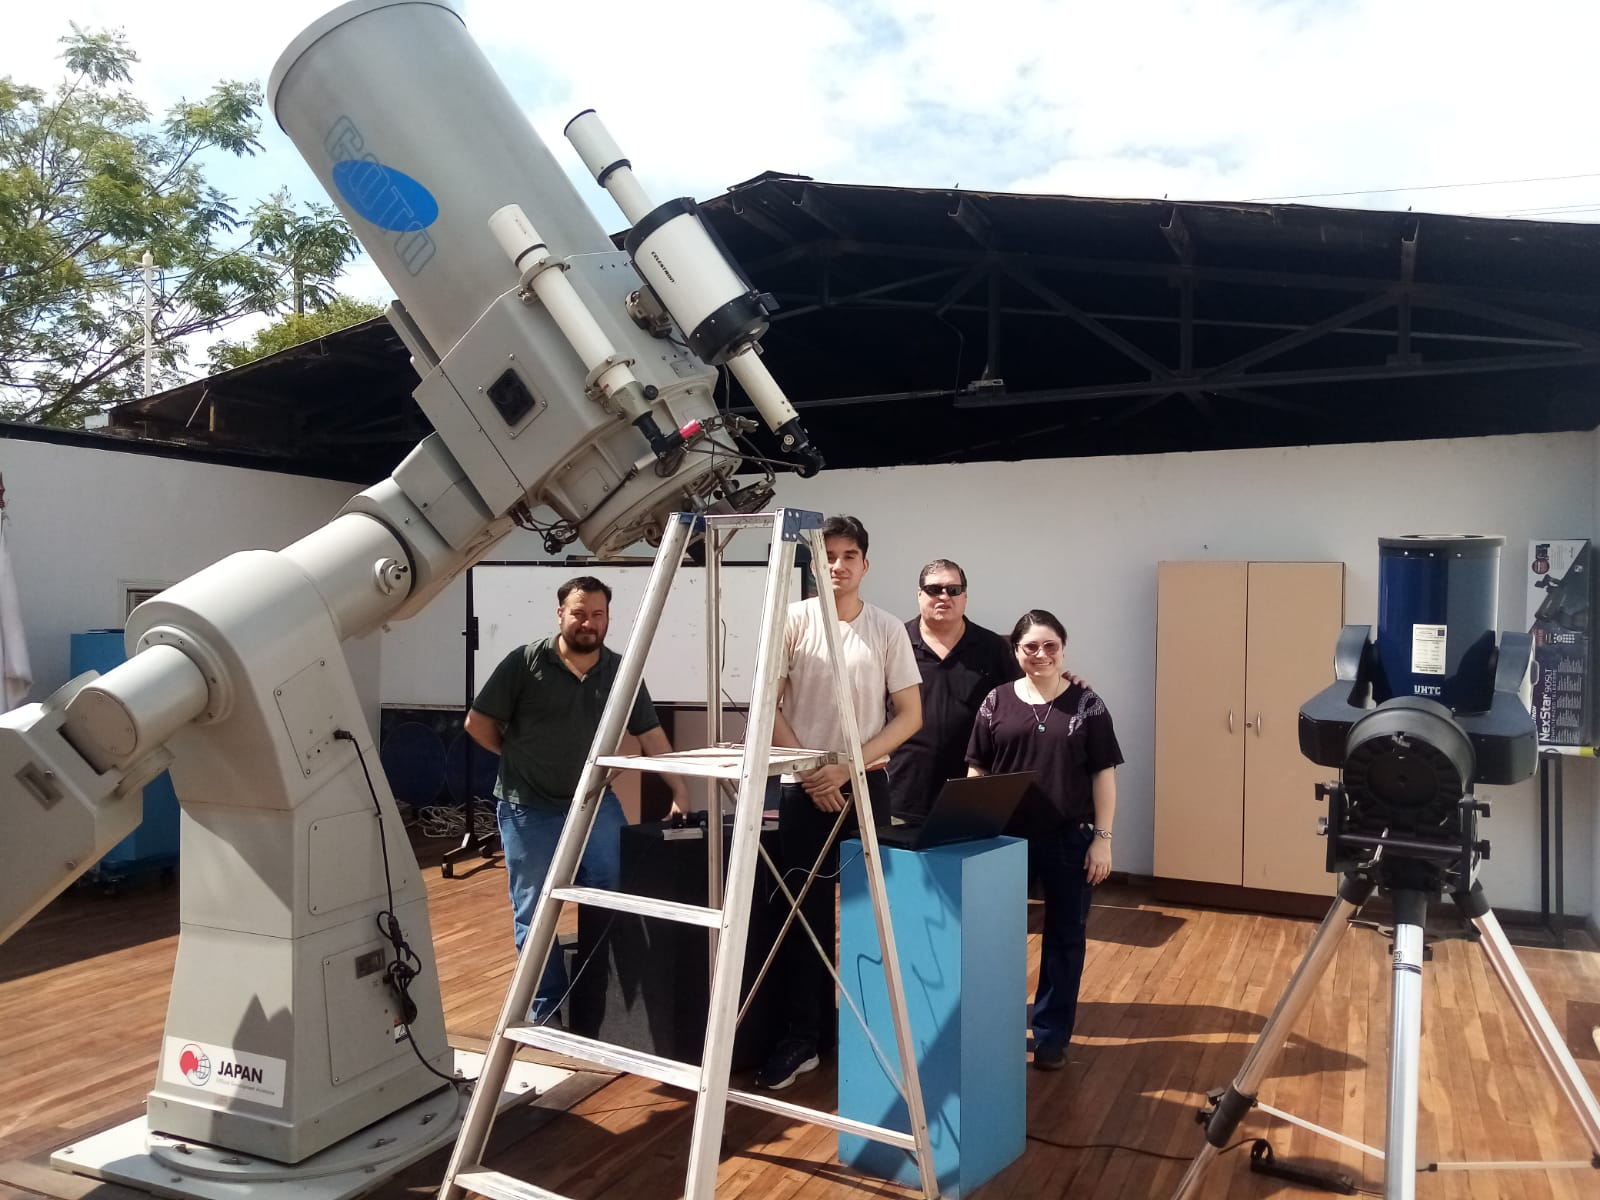
\includegraphics[height=0.75\textheight, width=\linewidth, keepaspectratio]{hw/telescope_team.jpg}
        \end{column}
        
        % Columna Derecha: Bloques de Trabajo Futuro y Recomendaciones técnicos y objetivos
        \begin{column}{0.56\textwidth}
            \scriptsize
            
            % Bloque 1: Trabajo Futuro (Conversión de la tabla a un formato más compacto y limpio)
            \begin{block}{Trabajo futuros}
                \begin{itemize}
                    \item \textbf{Datos y Óptica:} Expandir campañas observacionales locales y automatizar las rutinas de enfoque y exposición del hardware.
                    \item \textbf{Modelos y Validación:} Optimizar la ejecución en el borde mediante cuantización fina en ONNX y contrastar resultados con anotaciones manuales.
                \end{itemize}
            \end{block}
            
            \vspace{0.1cm}
            
            % Bloque 2: Recomendaciones (Incorporación rigurosa sobre el análisis de PCA)
            \begin{block}{Recomendaciones metodológicas}
                \begin{itemize}
                    \item \textbf{Análisis de sensibilidad en PCA:} Evaluar la reducción dimensional bajo análisis de sensibilidad estadístico para estimar el número óptimo de componentes principales.
                    \item \textbf{Robustez del modelo:} Incrementar el volumen de observaciones locales con el fin de mitigar el sesgo y mejorar la transferencia de dominio del sistema.
                \end{itemize}
            \end{block}
            
        \end{column}
    \end{columns}
\end{frame}

\begin{frame}{Agradecimientos Institucionales}
    \begin{center}
        \begin{columns}
            \begin{column}{0.5\textwidth}
                \centering
                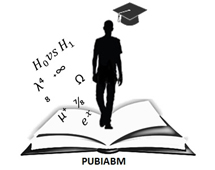
\includegraphics[width=0.6\textwidth]{logos/pubiam_logo.jpg}
                \vskip 10pt
                %{\footnotesize Financiación parcial a través de la beca PUBIABM.}
            \end{column}
            \begin{column}{0.6\textwidth}
                \centering
                
\includegraphics[width=0.7\textwidth]{logos/observario_logo.png}
                \vskip 10pt
                %{\footnotesize Soporte e infraestructura del Observatorio Alexis Troche Boggino.}
            \end{column}
        \end{columns}
    \end{center}
\end{frame}

\begin{frame}
    \begin{center}
        {\Huge Gracias}

        \vspace{0.5cm}
        \large Consultas y observaciones
    \end{center}
\end{frame}

\end{document}